\documentclass[a4paper, 10pt]{article}
\usepackage[margin=1in]{geometry}
\usepackage{amsfonts, amsmath, amssymb, amsthm}
%\usepackage[none]{hyphenat}
\usepackage{fancyhdr} %create a custom header and footer
\usepackage[utf8]{inputenc}
\usepackage[english, main=ukrainian]{babel}
\usepackage{pgfplots}
\pgfplotsset{compat = newest}
\usepgfplotslibrary{fillbetween}
\usepackage{tikz}
\usepackage{graphicx}
\usepackage[scr]{rsfso}
\usepackage[autostyle]{csquotes}
\usepackage{physics}
\usepackage{float}
\usepackage[unicode]{hyperref}
\usepackage{caption}
\usepackage{scalerel,stackengine}
\stackMath
\newcommand\reallywidehat[1]{%
\savestack{\tmpbox}{\stretchto{%
  \scaleto{%
    \scalerel*[\widthof{\ensuremath{#1}}]{\kern-.6pt\bigwedge\kern-.6pt}%
    {\rule[-\textheight/2]{1ex}{\textheight}}%WIDTH-LIMITED BIG WEDGE
  }{\textheight}% 
}{0.5ex}}%
\stackon[1pt]{#1}{\tmpbox}%
}
%\usepackage{ragged2e}
\usepackage[shortcuts]{extdash}


\fancyhead{}
\fancyfoot{}
\parindent 0ex
\DeclareMathOperator*\uplim{\overline{lim}}
\def\stackbelow#1#2{\underset{\displaystyle\overset{\displaystyle\shortparallel}{#2}}{#1}}
\def\residue#1#2{\underset{z = {#1}}{\textrm{res}} {#2}}
\def\residuee#1#2{\underset{p = {#1}}{\textrm{res}} {#2}}
\def\hugespace{\vspace{5mm} \\}

\usepackage{blindtext}

\def\qed{$\blacksquare$}

\def\rightproof{$\boxed{\Rightarrow}$ }
\def\leftproof{$\boxed{\Leftarrow}$ }


\def\noProof{\\ \textit{Без доведення.}}
\DeclareMathOperator\sign{sgn}

\newtheoremstyle{theoremdd}% name of the style to be used
  {\topsep}% measure of space to leave above the theorem. E.g.: 3pt
  {\topsep}% measure of space to leave below the theorem. E.g.: 3pt
  {\normalfont}% name of font to use in the body of the theorem
  {0pt}% measure of space to indent
  {\bfseries}% name of head font
  {}% punctuation between head and body
  { }% space after theorem head; " " = normal interword space
  {\thmname{#1}\thmnumber{ #2}\textnormal{\thmnote{ \textbf{#3}\\}}}

\theoremstyle{theoremdd}
\newtheorem{theorem}{Theorem}[subsection]
  
\theoremstyle{theoremdd}
\newtheorem{definition}[theorem]{Definition}

\theoremstyle{theoremdd}
\newtheorem{samedef}[theorem]{Definition}

\theoremstyle{theoremdd}
\newtheorem{example}[theorem]{Example}

\theoremstyle{theoremdd}
\newtheorem{proposition}[theorem]{Proposition}

\theoremstyle{theoremdd}
\newtheorem{remark}[theorem]{Remark}

\theoremstyle{theoremdd}
\newtheorem{lemma}[theorem]{Lemma}

\theoremstyle{theoremdd}
\newtheorem{corollary}[theorem]{Corollary}

\makeatletter
\renewenvironment{proof}[1][Proof.\\]{\par
\pushQED{\hfill \qed}%
\normalfont \topsep6\p@\@plus6\p@\relax
\trivlist
\item\relax
{\bfseries
#1\@addpunct{.}}\hspace\labelsep\ignorespaces
}{%
\popQED\endtrivlist\@endpefalse
}
\makeatother

\newenvironment{pfMI}{\vspace*{-3mm} \textbf{\\ Proof MI. \\}}{\hfill $\blacksquare$}
\newenvironment{pfNoTh}{\textbf{Proof. \\}}{$\blacksquare$}

\newcommand\Norm[1]{\lVert#1\rVert}

\newcommand{\notimplies}{\;\not\!\!\!\implies}
\def\departial#1#2{\dfrac{\partial {#1}}{\partial {#2}}}
\def\seconddepartial#1#2#3{\ifthenelse{\equal{#2}{#3}}{\dfrac{\partial^2 {#1}}{\partial {#2}^2}}{\dfrac{\partial^2 {#1}}{\partial {#2} \partial {#3}}}}
\def\huge{\displaystyle}
\DeclareMathOperator{\Ln}{Ln}



\begin{document}
\tableofcontents
\newpage
	
\section{Комплексні числа}
\subsection{Вступ}
Комплексним числом будемо називати число такого формату:
\begin{align*}
a + ib
\end{align*}
Тут $a,b \in \mathbb{R}$. А число $i$ називають \textbf{уявною одиницею} - це таке число, що
\begin{align*}
i^2 = -1
\end{align*}
Множину комплексних чисел ми позначимо за $\mathbb{C}$.

\subsubsection*{Коли комплексні числа рівні}
Якщо у нас є два комплексних числа $a_1 + ib_1$ та $a_2 + ib_2$, то тоді
$$a_1 + ib_1 = a_2 + ib_2 \iff \begin{cases} a_1 = a_2 \\ b_1 = b_2 \end{cases}$$
Інтуїтивне пояснення буде згодом, чому саме так.

\subsubsection*{Основна арифметика}
Ми можемо два комплексних числа довадати/віднімати, множити та ділити. Тобто якщо маємо $a_1 + ib_1$ та $a_2 + ib_2$ то\\
$(a_1+ib_1) \pm (a_2 + ib_2) = (a_1 \pm a_2) + i(b_1 \pm b_2)$
\bigskip \\
$(a_1+ib_1) \cdot (a_2 + ib_2) = a_1 a_2 + a_1 i b_2 + ib_1 a_2 + i^2 b_1 b_2 = (a_1a_2-b_1b_2) + i(a_1b_2+a_2b_1)$
\bigskip \\
Із діленням ситуація цікавіша. Для числа $z = a+bi$ введемо поняття \textbf{комплексно спряжене число} - це комплексне число такого формату:
\begin{align*}
\bar{z} = a - ib
\end{align*}

\begin{example}
Маємо $z = 3 + 4i$. Спряженим буде $\bar{z} = 3 - 4i$.
\end{example}

Якщо тепер перемножити стандартне комплексне число на його спряжене, то ми отримаємо наступне:
\begin{align*}
(a+ib)(a-ib) = a^2 - (ib)^2 = a^2 + b^2
\end{align*}
Ідея ділення двох комплексних чисел полягає в домноженні дроба на комплексно спряжене число знаменника, тобто:\\
$\dfrac{a_1+ ib_1}{a_2 + ib_2} = \dfrac{(a_1 + ib_1)\textcolor{red}{(a_2-ib_2)}}{(a_2+ib_2)\textcolor{red}{(a_2-ib_2)}} = \dfrac{(a_1a_2 + b_1b_2) + i(a_2b_1-a_1b_2)}{a_2^2 + b_2^2} = \dfrac{a_1a_2 + b_1b_2}{a_2^2 + b_2^2} + i \dfrac{a_2 b_1 - a_1 b_2}{a_2^2 + b_2^2}$.

\begin{example}
$\dfrac{2+3i}{1-i} = \dfrac{(2+3i) \cdot \textcolor{red}{(1+i)}}{(1-i) \cdot \textcolor{red}{(1+i)}} = \dfrac{2+2i+3i+3i^2}{1^2-i^2} = \dfrac{2+5i-3}{2} = \dfrac{-1+5i}{2} = -\dfrac{1}{2} + \dfrac{5}{2}i$.
\end{example}

\subsection{Геометрична інтерпретація та ще трохи арифметики}
Нехай є комплексне число $z = x + iy, \hspace{0.5cm} x,y \in \mathbb{R}$. Уведемо нові позначення:\\
$x = \Re z$ - цю частину комплексного числа називають ще \textbf{дійсною частиною}. \\
$y = \Im z$ - цю частину комплексного числа називають ще \textbf{уявною частиною}.\\
Нагадаю, що комплексно спряжене до числа $z$ позначаємо так: $\bar{z} = x - iy$.
\bigskip \\
Копмлексне число можна інтерпретувати як \enquote{вектор} на такій системі координат:
\begin{figure}[H]
\centering
\begin{tikzpicture}
\draw[thick, ->] (-3,0)--(4,0) node[anchor = north] {$x = \Re z$};
\draw[thick, ->] (0,-2)--(0,4) node[anchor = east] {$y = \Im z$};
\draw[thick, dashed] (-2,2)--(0,2) node[anchor = west] {$y$};
\draw[thick, dashed] (-2,2)--(-2,0) node[anchor = north] {$x$};
\draw[thick, ->, red] (0,0)--(-2,2) node[anchor = south] {$z$};
\draw[black] (0.5,0) arc (0:135:0.5) node at (0.5,0.5) {$\varphi$};
\draw node at (0.2,-0.3) {$0$};
\end{tikzpicture}
\end{figure}
Можемо знайти \textbf{довжину} комплексного числа - відстань до початку координат
$$|z| = \sqrt{x^2+y^2}$$
Із цього випливає наступна формула:\\
$z \cdot \bar{z} = (x+iy)(x-iy) = x^2+y^2 = |z|^2$.
\bigskip \\
Ще одне нове позначення:\\
$\varphi = \arg z$ - \textbf{аргумент комплексного числа}. Зазвичай $\varphi \in (-\pi,\pi]$.
\bigskip \\
При $z = 0$ маємо $|z| = 0$, а тому звідси $\arg z = ?$. Тому надалі уникаємо тут випадок $z = 0$.
\bigskip \\
Повернімось до малюнку вище та спробуємо знайти $x,y$. За геометрічними міркуваннями:\\
$\begin{cases}
x = |z| \cos \varphi \\
y = |z| \sin \varphi
\end{cases}
$\\
Такі значення $x,y$ ми підставимо в комплексне число $z = x + iy$.\\ Отримаємо \textbf{тригонометричну формулу} комплексного числа:
$$z = |z|(\cos \varphi + i \sin \varphi)$$
З'ясуємо арифметику комплексних чисел в тригонометричній формулі. Нехай є 2 комплексних числа:\\
$z_1 = |z_1| (\cos \varphi_1 + i \sin \varphi_1)$\\
$z_2 = |z_2| (\cos \varphi_2 + i \sin \varphi_2)$

\subsubsection*{Множення}
\begin{flalign*}
z_1 \cdot z_2 & = |z_1| |z_2| (\cos \varphi_1 + i \sin \varphi_2) (\cos \varphi_1 + i \sin \varphi_2) \\ & = |z_1| |z_2| (\cos \varphi_1 \cos \varphi_2 - \sin \varphi_1 \sin \varphi_2 + i[\sin \varphi_1 \cos \varphi_2 + \sin \varphi_2 \cos \varphi_1]) && \\ &
= |z_1||z_2|(\cos (\varphi_1 + \varphi_2) + i \sin(\varphi_1 + \varphi_2)) &&
\end{flalign*}

Отримали, що коли ми множимо два комплексних числа, модулі ми \textbf{множимо}, а аргументи ми \textbf{додаємо}, тобто\\
$\begin{cases}
|z_1 \cdot z_2| = |z_1| \cdot |z_2| \\
\arg(z_1 \cdot z_2) = \arg z_1 + \arg z_2
\end{cases}$\\
$z_1 \cdot z_2 = |z_1||z_2|(\cos (\varphi_1 + \varphi_2) + i \sin(\varphi_1 + \varphi_2))$

\subsubsection*{Ділення}
$\dfrac{z_1}{z_2} \overset{\textrm{позначу}}{=} w$, де $w = |w|(\cos \psi + i \sin \psi)$.\\
Наша мета: знайти $|w|$ та $\arg w = \psi$.\\
Ми вже навчилися множити два комплексних числа в тригонометричній формі, тому зведемо таким чином:\\
$z_1 = w z_2 \implies \begin{cases} |z_1| = |z_2| \cdot |w| \\ \arg z_1 = \arg z_2 + \arg w \end{cases} \implies \begin{cases} |z_1| = |z_2| \cdot |w| \\ \varphi_1 = \varphi_2 + \psi \end{cases}$\\
Я тут позначив $\arg z_1 = \varphi_1 \hspace{1cm} \arg z_2 = \varphi_2$.\\
Звідси знайдемо, чому дорівнює $|w|$ та $\psi$:\\
$\begin{cases} |w| = \dfrac{|z_1|}{|z_2|} \\ \psi = \varphi_1 - \varphi_2 \end{cases}$\\
В результаті оскільки $w = |w| (\cos \psi + i \sin \psi)$, ми отримаємо:\\
$w = \dfrac{z_1}{z_2} = \dfrac{|z_1|}{|z_2|} (\cos (\varphi_1 - \varphi_2) + i \sin (\varphi_1 - \varphi_2))$.\\
Отримали, що коли ми ділимо два комплексних числа, модулі ми \textbf{ділимо}, а аргументи ми \textbf{віднімаємо}.

\subsubsection*{Зведення в степінь}
$z^n \overset{\text{позначу}}{=} w$, де $w = |w|(\cos \psi + i \sin \psi)$.\\
Знову наша мета: знайти $|w|$ та $\arg w = \psi$.\\
Оскільки $w = z \underset{\text{n разів}}{\cdots} z$, то за множенням комплексним чисел, маємо, що $\begin{cases} |w| = |z| \underset{\text{n разів}}{\cdots} |z| \\ \arg w = \arg z + \underset{\text{n разів}}{\dots} + \arg z  \end{cases} \\ \implies \begin{cases} |w| = |z|^n \\ \arg w = n \arg z = n \varphi \end{cases}$.\\
В результаті отримали \textbf{формулу Муавра}:
\begin{align*}
z^n = |z|^n (\cos (n \varphi) + i \sin (n \varphi))
\end{align*}

\begin{remark}
Вважаємо, що $z^0 = 1$ при $z \neq 0$.
\end{remark}

\subsubsection*{Вилучення коренів}
\begin{definition}
Комплексне число $w$ буде \textbf{$n$-м коренем від $z$}, якщо $w^n = z$.\\
Позначення: $w = \sqrt[n]{z}$.
\end{definition}

$\sqrt[n]{z} \overset{\textrm{позн.}}{=} w$, де $w = |w|(\cos \psi + i \sin \psi)$.\\
Ще раз мета: знайти $|w|$ та $\arg w = \psi$.\\
Ми щойно навчилися зводити комплексне число в степінь, тому зведемо таким чином:\\
$z = w^n$.\\
$z = |z|(\cos \varphi + i \sin \varphi) = |w|^n (\cos n \psi + i \sin n \psi) = w^n$.\\

Отримаємо, що $\begin{cases} |w|^n = |z| \\ n \psi = \varphi + 2 \pi k \end{cases} \implies \begin{cases} |w| = \sqrt[n]{|z|} \\ \psi = \dfrac{\varphi + 2\pi k}{n} \end{cases}$.\\
Більш детальне пояснення другого рівняння системи.\\
Ми мали, що $\cos \varphi = \cos (n \psi)$. Оскільки $\cos$ - $2\pi$-періодична функція, то нас влаштовують не лише $\varphi = n \psi$, а також кути $+2\pi$, $+4\pi$, $\dots$.\\
В результаті отримаємо:
$$w = \sqrt[n]{z} = \sqrt[n]{|z|} \left(\cos \dfrac{\varphi + 2\pi k}{n} + i \sin \dfrac{\varphi + 2 \pi k}{n} \right), \hspace{0.5cm} k = 0,1,\dots,n-1$$
Якщо $k = n$, то ми отримаємо комплексне число для випадку $k = 0$ через періодичність тригонометричних функцій\\
Якщо $k = n+1$, то ми отримаємо комплексне число для випадку $k = 1$ через періодичність тригонометричних функцій\\
Тощо...\\
Якщо $k = -1$, то ми отримаємо комплексне число для випадку $k = n-1$ через періодичність тригонометричних функцій\\
Тощо...\\
Отже:

\begin{proposition}
$\sqrt[n]{z}$ має рівно $n$ комплексних чисел при $z \neq 0$.
\end{proposition}

\begin{example}
Знайти $\sqrt[3]{i}$.\\
Розпишемо $i = 0 + i \cdot 1$. Якщо це намалювати на площині, то отримаємо, що \\ $|i| = \sqrt{0^2+1^2} = 1, \hspace{0.5cm} \arg i = \varphi = \dfrac{\pi}{2}$.
\begin{figure}[H]
\centering
\begin{tikzpicture}
\draw[thick, ->] (-2,0)--(3,0) node[anchor = north] {$x = \Re z$};
\draw[thick, ->] (0,-2)--(0,2) node[anchor = east] {$y = \Im z$};
\draw[thick, ->, red] (0,0)--(0,1) node[anchor = south west] {$z = i$};
\draw[black] (0.5,0) arc (0:90:0.5) node at (1.2,0.5) {$\varphi = \dfrac{\pi}{2}$};
\draw node at (0.2,-0.3) {$0$};
\end{tikzpicture}
\end{figure}
А тепер витягуємо корінь:\\
$\sqrt[3]{i} = \sqrt[3]{1} \left( \cos \dfrac{\dfrac{\pi}{2} + 2 \pi k}{3} + i \sin \dfrac{\dfrac{\pi}{2} + 2 \pi k}{3} \right), \hspace{0.5cm} k=0,1,2$\\
$k = 0 \implies \cos \dfrac{\pi}{6} + i \sin \dfrac{\pi}{6} = \dfrac{\sqrt{3}}{2} + \dfrac{1}{2}i$\\
$k = 1 \implies \cos \dfrac{5 \pi}{6} + i \sin \dfrac{5 \pi}{6} = -\dfrac{\sqrt{3}}{2} + \dfrac{1}{2}i$\\
$k = 2 \implies \cos \dfrac{3 \pi}{2} + i \sin \dfrac{3 \pi}{2} = -i$
\begin{figure}[H]
\centering
\begin{tikzpicture}
\draw[thick, ->] (-2,0)--(3,0) node[anchor = north] {$x = \Re z$};
\draw[thick, ->] (0,-2)--(0,2) node[anchor = east] {$y = \Im z$};
\draw[thick, ->, red] (0,0)--(0,-1) node[anchor = south west] {$z = -i$};
\draw[thick, ->, red] (0,0)--({sqrt(3)/2},{1/2}) node[anchor = south west] {$z = \dfrac{\sqrt{3}}{2} + \dfrac{1}{2}i$};
\draw[thick, ->, red] (0,0)--({-sqrt(3)/2},{1/2}) node[anchor = south east] {$z = - \dfrac{\sqrt{3}}{2} + \dfrac{1}{2}i$};
\draw node at (0.2,-0.3) {$0$};
\end{tikzpicture}
\end{figure}
\end{example}

\subsection{Квадратні рівняння}
Одна з головних мотивацій створення комплексних чисел - це квадратне рівняння $x^2 = -1$.\\
В дійсних числах казали, що розв'язків нема. І дійсно, яке б ми число не зводили в квадрат, ми завжди отримуємо додатне число. Наразі ситуація змінюється і ми навчилися вилучати від'ємні корені. В результаті, \\
$x = \sqrt{-1} = \pm i$.

\begin{remark}
Там не випадково не написано $\pm$ перед коренем, тому що
\begin{flalign*}
\sqrt{z} & = \sqrt{|z|} \left( \cos \dfrac{\varphi + 2 \pi k}{n} + i \sin \dfrac{\varphi + 2 \pi k}{n} \right) = \left[ \begin{gathered} \sqrt{|z|} \left(\cos \dfrac{\varphi}{2} + i \sin \dfrac{\varphi}{2} \right) \\ \sqrt{|z|} \left(-\cos \dfrac{\varphi}{2} - i \sin \dfrac{\varphi}{2} \right) \end{gathered} \right. = \pm \sqrt{|z|} \left(\cos \dfrac{\varphi}{2} + i \sin \dfrac{\varphi}{2} \right) &&
\end{flalign*}
Тобто, вилучаючи квадратний корінь, ми вже отримуємо два значення, тобто виникає $\pm$ після цього процесу. Але тепер можна спокійно розв'язувати квадратні рівняння.
\end{remark}

$az^2 + bz + c = 0$\\
$a \left( z^2 + \dfrac{2b}{2a}z + \left(\dfrac{b}{2a} \right)^2 \right) + c - \dfrac{b^2}{4a} = 0$\\
$a \left(z + \dfrac{b}{2a} \right)^2 = \dfrac{b^2-4ac}{4a}$\\
$\left(z + \dfrac{b}{2a} \right)^2 = \dfrac{b^2-4ac}{4a^2}$\\
$z + \dfrac{b}{2a} = \pm \dfrac{\sqrt{b^2-4ac}}{2a}$\\
$z = \dfrac{-b\pm \sqrt{D}}{2a}$

\subsection{Первинні результати}
\begin{proposition}
Задані два комплексних числа $z,w$. Тоді\\
1. $\overline{z+w} = \bar{z} + \bar{w}$;\\
2. $\overline{zw} = \bar{z} \bar{w}$;\\
3. $|zw| = |z| |w|$.
\end{proposition}

\begin{proof}
Ми маємо $z = x_1 + iy_1$ та $w = x_2 + iy_2$. Тоді звідси\\
$z+w = (x_1+x_2) + i (y_1+y_2)$\\
$zw = (x_1x_2-y_1y_2) + i(x_1y_2+x_2y_1)$.\\
$|zw| = \sqrt{(x_1x_2-y_1y_2)^2 + (x_1y_2+x_2y_1)^2}$.\\
А далі вже доводимо ці тотожності вище:\\
1. $\overline{z+w} = (x_1+x_2) - i (y_1+y_2) = (x_1 - iy_1) + (x_2-1y_2) = \bar{z} + \bar{w}$.\\
2. $\overline{zw} = (x_1x_2-y_1y_2) - i(x_1y_2+x_2y_1) =(x_1-iy_1)(x_2-iy_2) = \bar{z} \bar{w}$.\\
3. $|zw|^2 = x_1^2x_2^2+y_1^2y_2^2+x_1^2y_2^2+x_2^2y_1^2 = x_1^2(x_2^2+y_2^2) + y_1^2(x_2^2+y_2^2) = |z|^2 |w|^2$.
\end{proof}

\begin{proposition}[Нерівність трикутника]
Задані два комплексних числа $z,w$. Тоді
$|z+w| \leq |z| + |w|$.
\end{proposition}

\begin{proof}
Хочемо довести, що $|z+w|^2 \leq (|z|+|w|)^2$.\\
Спочатку зауважимо, що $|z+w|^2 = (z+w)\overline{(z+w)} = (z+w)(\bar{z}+\bar{w})$.\\
Далі просто розкриємо дужки в правій частині:\\
$(z+w)(\bar{z}+\bar{w}) = |z|^2 + |w|^2 + z\bar{w} + w\bar{z} = |z|^2 + |w|^2 + z \bar{w} + \overline{z \bar{w}} = |z|^2 + |w|^2 + 2 \Re (z \bar{w})$.\\
Маємо $\Re (z \bar{w}) \in \mathbb{R}$, а тому звідси $\Re (z \bar{w}) \leq |\Re (z \bar{w})| \leq |z \bar{w}|$.\\
Дійсно, $\Re (a+bi) \leq |a+bi|$, тому що $\Re (a+bi) = a = \sqrt{a^2} \leq \sqrt{a^2+b^2} = |a+bi|$.\\
Отже, $|z+w|^2 \leq |z|^2 + |w|^2 + 2|z \bar{w}| = |z|^2 + |w|^2 + 2|z| |w| = (|z|+|w|)^2$.
\end{proof}

Решта нерівностей, що пов'язані з модулями, також тут працюють. Просто тому що ми довели нерівність трикутника.

\iffalse
\subsection{Показникова формула}
Коли ми множимо два комплексних числа, то аргументи ми додаємо, тобто\\
$(\cos \varphi + i \sin \varphi)(\cos \psi + i \sin \psi) = \cos (\varphi + \psi) + i \sin (\varphi + \psi)$\\
Додавання при множенні виявляється під час робтою зі степенями, справді:\\
$a^x a^y = a^{x+y}$.\\
Така паралель буде мотивацією нової форми комплексного числа.

\begin{definition}
Нехай $z = |z|(\cos \varphi + i \sin \varphi)$.\\
\textbf{Показникова форма} числа $z$ має такий вигляд:
\begin{align*}
z = |z|e^{i \varphi}
\end{align*}
Ось тут $e \approx 2.71$ - число Ейлера.
\end{definition}

Якщо в це рівняння підставити $z = |z|(\cos \varphi + i \sin \varphi)$ - її тригонометричну формулу - звідси отримаємо \textbf{формулу Ейлера}
$$ e^{i \varphi} = \cos \varphi + i \sin \varphi $$
Запишемо формулу Ейлера:\\
$e^{i \varphi} = \cos \varphi + i \sin \varphi$ $(1)$\\
Підставимо в цю формулу $-\varphi$, отримаємо:\\
$e^{-i \varphi} = \cos \varphi - i \sin \varphi$ $(2)$\\
$(1) + (2) \implies \cos \varphi = \dfrac{e^{i \varphi} + e^{-i \varphi}}{2}$\\
$(1) - (2) \implies \sin \varphi = \dfrac{e^{i \varphi} - e^{-i \varphi}}{2i}$.
\fi
\newpage

\section{Числові послідовності, функції, границі та неперервність}
\subsection{Числові послідовності}
\begin{definition}
\textbf{Послідовністю} комплексних чисел назвемо набір чисел $\{z_n, n \geq 1\}$, де $z_n \in \mathbb{C}$.
\end{definition}

\begin{definition}
Число $z \in \mathbb{C}$ називається \textbf{границею} числової послідовності $\{z_n, n \geq 1\}$, якщо
\begin{align*}
\forall \varepsilon > 0: \exists N \in \mathbb{N}: \forall n \geq N: |z_n-z| < \varepsilon
\end{align*}
Дану числову послідовність будемо називати \textbf{збіжною}, якщо ліміт існує та $z \in \mathbb{C}$. У протилежному випадку - \textbf{розбіжною}.
\end{definition}

\begin{proposition}
Задано $\{z_n, n \geq 1\}$ - числова послідовність, де $z_n + x_n + iy_n$, та $z = x+iy,z \in \mathbb{C}$.\\
$\exists \displaystyle\lim_{n \to \infty} z_n = z\iff \begin{cases} \displaystyle \exists \lim_{n \to \infty} x_n = x \\ \exists \displaystyle  \lim_{n \to \infty} y_n = y \end{cases}$.
\end{proposition}

\begin{proof}
$\exists \displaystyle\lim_{n \to \infty} = z \iff \forall \varepsilon > 0: \exists N: \forall n \geq N: |z_n-z| < \varepsilon \iff |z_n-z| = \sqrt{(x_n-x)^2 + (y_n-y)^2} < \varepsilon \iff \\ \iff \begin{cases} |x_n-x| < \varepsilon \\ |y_n-y| < \varepsilon \end{cases} \iff \exists \displaystyle \lim_{n \to \infty} x_n = x, \exists \lim_{n \to \infty} y_n = y$.\\
Хіба шо в зворотному напрямку там будуть існувати $N_1,N_2$ для кожного ліміту, але можна потім записати $N = \max\{N_1,N_2\}$.
\end{proof}

\begin{definition}
Числова послідовність $\{z_n, n \geq 1\}$ називається \textbf{фундаментальною}, якщо
\begin{align*}
\forall \varepsilon > 0: \exists N \in \mathbb{N}: \forall m,n \geq N: |z_n-z_m| < \varepsilon
\end{align*}
\end{definition}

\begin{lemma}
Послідовність $\{z_n, n \geq 1\}$ - фундаментальна $\iff \{x_n, n \geq 1\}, \{y_n,n \geq 1\}$ - фундаментальні.\\
У цьому випадку $z_n = x_n + iy_n$.\\
\textit{Аналогічно доводиться, як попереднє твердження.}
\end{lemma}

\begin{theorem}[Критерій Коші]
Послідовність $\{z_n, n \geq 1\}$ - збіжна $\iff \{z_n, n \geq 1\}$ - фундаментальна.\\
\textit{Доведення зрозуміле.}
\end{theorem}

\begin{definition}
Числова послідовність $\{z_n, n \geq 1\}$ називається \textbf{обмеженою}, якщо
\begin{align*}
\exists C > 0: \forall n \geq 1: |z_n| \leq M
\end{align*}
\end{definition}

\begin{proposition}
Задано послідовність $\{z_n, n \geq 1\}$ - збіжна. Тоді вона - обмежена.\\
\textit{Доведення аналогічне, як в матані $\mathbb{R}$.}
\end{proposition}

\begin{proposition}
Задані послідовності $\{z_n^{(1)}, n \geq 1\}$ та $\{z_n^{(2)}, n \geq 1\}$ - збіжні. Тоді $\{z_n^{(1)}+z_n^{(2)}, n \geq 1\}, \{\lambda z_n^{(1)}, n \geq 1 \}, \lambda \in \mathbb{C}$, $\{z_n^{(1)} \cdot z_n^{(2)}, \geq 1\}$ та $\left\{ \dfrac{z_n^{(1)}}{z_n^{(2)}}, \geq 1 \right\}$ (тут якщо ліміт для $z_n^{(2)}$ ненулевий) - збіжні, причому:\\
$\displaystyle\lim_{n \to \infty} (z_n^{(1)} + z_n^{(2)}) = \lim_{n \to \infty} z_n^{(1)} + \lim_{n \to \infty} z_n^{(2)}$.\\
$\displaystyle\lim_{n \to \infty} (\lambda z_n^{(1)}) = \lambda \lim_{n \to \infty} z_n^{(1)}$.\\
$\displaystyle\lim_{n \to \infty} (z_n^{(1)} z_n^{(2)}) = \lim_{n \to \infty} z_n^{(1)} \lim_{n \to \infty} z_n^{(2)}$.\\
$\displaystyle\lim_{n \to \infty} \dfrac{z_n^{(1)}}{z_n^{(2)}} = \dfrac{\displaystyle\lim_{n \to \infty} z_n^{(1)}}{\displaystyle\lim_{n \to \infty} z_n^{(2)}}$.\\
\textit{Доведення неважке.}
\end{proposition}

\begin{proposition}[Достатня умова збіжності]
Задано $\{z_n, n \geq 1\}$ - числова послідовність. Представимо в вигляді $z_n = \rho_n e^{i \varphi_n}$, де $\rho_n = |z_n|$ та $\varphi_n = \arg z_n$. Відомо, що $\rho_n \to \rho_0, \varphi_n \to \varphi_0$ при $n \to \infty$.\\
Тоді $z_n \to z_0 = \rho_0 e^{i\varphi_0}$ при $n \to \infty$.
\end{proposition}

\begin{proof}
$|z_n - z_0| = |\rho_n e^{i\varphi_n} - \rho_0 e^{i \varphi_0}| \overset{\text{самостійно}}{=} \sqrt{\rho_n^2 + \rho_0^2 - 2 \rho_n \rho_0 \cos (\varphi_n-\varphi_0)} \boxed{\to}$\\
Оскільки $\varphi_n \to \varphi_0, n \to \infty$, то в силу неперервності $\cos x$ як дійснозначної функції маємо $\cos (\varphi_n - \varphi_0) \to 1, n \to \infty$.\\
Також $\sqrt{x}$ неперервна функція як дійснозначна функція, тому можна отримати ось таке прямування.\\
$\boxed{\to} \sqrt{\rho_0^2 + \rho_0^2 - 2 \rho_0 \rho_0 \cdot 1} = 0, n \to \infty$.
\end{proof}

\subsection{Функції комплексної змінної. Границі функцій}
Ми будемо розглядати \textbf{комплексні функції} $f: A \to \mathbb{C}$, де множина $A \subset \mathbb{C}$. Зазвичай позначають як $w = f(z)$.

\begin{example}
Розглянемо кілька прикладів:\\
$w = \bar{z}$ \hspace{1cm} $w = \Re z$ \hspace{1cm} $w = \Im z$.\\
Ці три функції визначені на $A = \mathbb{C}$
\end{example}

\begin{remark}
Маємо $z = x+iy$, а також функцію $f(z) = w = u + iv$.\\
Тоді задання функції $f(z)$ евківалентно заданню двох дійсних функцій $u(x,y),v(x,y)$. І тоді
$$ f(z) = f(x,y) = u(x,y) + iv(x,y),$$
де $\Re f(z) = u(x,y), \Im f(z) = v(x,y)$.
\end{remark}

\begin{example}
Зокрема маємо $f(z) = \bar{z}$, або це перепишеться як\\
$f(x,y) = x - iy$. У цьому випадку $u(x,y) = x, v(x,y) = -y$.
\end{example}

\begin{definition}
\textbf{Показникову функцію} $w = e^z, z = x + iy \in \mathbb{C}$ визначимо таким чином:
\begin{align*}
e^z = e^x(\cos y + i \sin y)
\end{align*}
Деколи це ще позначають як $w = \exp(z)$.
\end{definition}

\begin{proposition}[Властивості показникової функції]
1. $e^{z_1} \cdot e^{z_2} = e^{z_1+z_2}$ при $z_1 = x_1+iy_1$ та $z_2 = x_2+iy_2$.\\
2. $e^z$ - періодична, де $T = 2\pi i$.\\
3. $|e^z| = e^x$.\\
4. $\arg e^z = y$.\\
\textit{Доведення неважке.}
\end{proposition}

\begin{corollary}
$e^{2\pi n i} = 1$ \hspace{1cm} $e^{(2n+1)\pi i} = -1$.
\end{corollary}

\begin{definition}
Визначимо ще дві тригонометричні функції:
\begin{align*}
\sin z = \dfrac{e^{iz} - e^{-iz}}{2i} \\
\cos z = \dfrac{e^{iz} + e^{-iz}}{2}
\end{align*}
\end{definition}

\begin{proposition}[Властивості тригонометричних функцій]
1. $\sin z, \cos z$ - періодичні, де $T = 2\pi$.\\
2. $\sin z$ - непарна функція та $\cos z$ - парна функція.\\
\textit{Доведення неважке.}
\end{proposition}

\begin{remark}
Комплексні функції $\sin z, \cos z$ підпорядковуються стандартним тригонометричним тотожностям.
\end{remark}

\begin{corollary}[Формула Ейлера]
$e^{iz} = \cos z + i \sin z$, де $z \in \mathbb{C}$.
\end{corollary}

\begin{corollary}[Показникова форма комплексного числа]
$z = |z| e^{i \varphi}$, де $\varphi = \arg z$.
\end{corollary}

\begin{definition}
\textbf{Логарифмічну функцію} $w = \Ln z$ визначимо як функцію, для якого:
\begin{align*}
e^w = e^{\Ln z} = z
\end{align*}
Вона визначена всюди, окрім $z = 0$.
\end{definition}

Тепер розпишемо $e^w = z$ більш детально. Маємо $z = |z| e^{i\varphi}$ та $w = u+iv$, тоді\\
$e^{u} e^{iv} = |z| e^{i\varphi} \implies \begin{cases} e^u = |z| \\ v = \varphi + 2\pi k, k \in \mathbb{Z} \end{cases} \implies \begin{cases} u = \ln |z| \\ v = \varphi + 2\pi k, k \in \mathbb{Z} \end{cases}$.\\
В останній системі перша рівність - там всі числа дійсні. Тепер підставимо все отримане:\\
$w = \ln |z| + i\varphi + 2\pi i k, k \in \mathbb{Z}$.\\
Але нам відомо, що $\varphi = \arg z$, а тому ми отримаємо:
$$ \Ln z = \ln |z| = i \arg z + 2\pi i k , k \in \mathbb{Z}$$

\begin{proposition}[Властивості логарифма]
1. $\Ln (z_1 \cdot z_2) = \Ln z_1 + \Ln z_2$.\\
2. $\Ln \dfrac{z_1}{z_2} = \Ln z_1 - \Ln z_2$.\\
\textit{Доведення неважке.}
\end{proposition}

\begin{definition}
\textbf{Степеневу функцію} визначимо таким чином:
\begin{align*}
z^\alpha = e^{\alpha \Ln z}
\end{align*}
Тут степінь $\alpha \in \mathbb{C}$.
\end{definition}

\begin{definition}
Визначимо деякі гіперболічні функції. Зокрема гіперболічний \textbf{сінус, косінус, тангенс, котангенс}:
\begin{align*}
\sh z = \dfrac{e^z-e^{-z}}{2} \\
\ch z = \dfrac{e^z + e^{-z}}{2} \\ 
\th z = \dfrac{\sh z}{\ch z} \\
\cth z = \dfrac{\ch z}{\sh z}
\end{align*}
\end{definition}

\begin{definition}
Задано функцію $f: A \to \mathbb{C}$, де $z_0 \in \mathbb{C}$ - гранична точка $A$.\\
Число $W$ називається \textbf{границею функції $f$ в т. $z_0$}, якщо
\begin{align*}
\forall \varepsilon > 0: \exists \delta(\varepsilon)>0: \forall z \in A: z \neq z_0: |z-z_0| < \delta \implies |f(z) - W| < \varepsilon \text{ - за Коші} \\
\forall \{z_n, n \geq 1 \} \subset A: \forall n \geq 1: z_n \neq z_0: \lim_{n \to \infty} z_n = z_0 \implies \lim_{n \to \infty} f(z_n) = W \text{ - за Гейне}
\end{align*}
Позначення: $W = \displaystyle\lim_{z \to z_0} f(z)$.
\end{definition}

\begin{theorem}
Означення Коші $\iff$ Означення Гейне.\\
\textit{Доведення аналогічне, як в матані $\mathbb{R}$.}
\end{theorem}

\begin{remark}
Думаю, мені не варто писати властивості границь функцій, більшість з яких просто копіюються сюди.
\end{remark}

\begin{theorem}
Задано функцію $f: A \to \mathbb{C}$ та $z_0 \in \mathbb{C}$ - гранична точка $A$. Нехай $f(z) = u(x,y) + i v(x,y)$ при $z = x+iy$, $z_0 = z_0+iy_0$. Також нехай $W = a+bi$.\\
$\displaystyle\exists \lim_{z \to z_0} f(z) = W \iff \begin{cases} \displaystyle\exists \lim_{(x,y) \to (x_0,y_0)} u(x,y) = a \\ \displaystyle\exists \lim_{(x,y) \to (x_0,y_0)} v(x,y) = b \end{cases}$.\\
\textit{Випливає з означення Гейне та твердження про збіжність комплексної послідовності.}
\end{theorem}

\subsection{Неперервність функції}
\begin{definition}
Задано функцію $f: A \to \mathbb{C}$ та $z_0 \in A$ - гранична точка $A$.\\
Функція $f$ називається \textbf{неперервною в т. $z_0$}, якщо
\begin{align*}
\exists \lim_{z \to z_0} f(z) = f(z_0)
\end{align*}
Функція $f$ називається \textbf{неперервною на $A$}, якщо $\forall z_0 \in A: f$ - неперервна в т. $z_0$. Позначається як $f \in C(A)$.\\
Також в ізольованих точках функція $f$ неперервна.
\end{definition}

\begin{theorem}
Задано функцію $f: A \to \mathbb{C}$ та $z_0 = x_0 +iy_0 \in A$ - гранична точка $A$.\\
$f(z) = u(x,y) + iv(x,y)$ - неперервна в т. $z_0 \iff u,v$ - неперервні в т. $(x_0,y_0)$.\\
\textit{Зрозуміло.}
\end{theorem}

\begin{example}
Зокрема ось такі функції неперервні на $\mathbb{C}$:\\
1. $f(z) = C, C \in \mathbb{C}$;\\
2. $f(z) = az+b$;\\
3. $f(z) = z^n, n \in \mathbb{N}$;\\
4. $f(z) = e^z$;\\
5. $f(z) = \cos z, f(z) = \sin z$;\\
6. $f(z) = \sh z, f(z) = \ch z$.
\end{example}

\begin{definition}
Задано функцію $f: A \to \mathbb{C}$ та $z_0 \in A$ - гранична точка $A$.\\
Функція $f$ називається \textbf{рівномірно неперервною на $A$}, якщо
\begin{align*}
\forall \varepsilon > 0: \exists \delta(\varepsilon) > 0: \forall z_1,z_2 \in A: |z_1-z_2| < \delta \implies |f(z_1)-f(z_2)| < \varepsilon
\end{align*}
Позначення: $f \in C_{unif}(A)$.
\end{definition}

\begin{theorem}
Задано функцію $f \in C_{unif}(A)$. Тоді $f \in C(A)$.
\end{theorem}

\begin{theorem}[Теорема Кантора]
Задано функцію $f \in C(A)$, де $A$ - замкнена та обмежена множина. Тоді $f \in C_{unif}(A)$.
\end{theorem}

Всі ці теореми доводяться аналогічно, як в матані $\mathbb{R}$.

\subsection*{Кілька прикладів на це все}
\begin{example}
Довести, що $\displaystyle\lim_{n \to \infty} \dfrac{1}{n^p} = 0$, якщо $\Re p > 0$.\\
Маємо $\abs{\dfrac{1}{n^p}} = \abs{\dfrac{1}{n^{a+bi}}} = \abs{\dfrac{1}{n^a}} \abs{\dfrac{1}{n^{bi}}} = \abs{\dfrac{1}{n^a}} \abs{\dfrac{1}{e^{bi \Ln n}}} = \dfrac{1}{n^a} \to 0, n \to \infty$, просто тому що $a > 0$.\\
Таким чином, $\displaystyle\lim_{n \to \infty} \dfrac{1}{n^p} = 0$, якщо $\Re p > 0$.
\end{example}

\begin{example}
Довести, що $\displaystyle\lim_{n \to \infty} \left( 1 + \dfrac{z}{n} \right)^n = e^z$.\\
Маємо $z_n = \left( 1 + \dfrac{z}{n} \right)^n$, звідси отримаємо:\\
$|z_n| = \left(\sqrt{\left( 1 + \dfrac{x}{n} \right)^2 + \dfrac{y^2}{n^2}}\right)^n = \left( 1 + \dfrac{x^2+y^2+2xn}{n^2} \right)^{\frac{n}{2}} \to e^x$ при $n \to \infty$ (показати самостійно).\\
$\arg z_n = \arg \left( 1 + \dfrac{z}{n} \right)^n = n \arg \left( 1 + \dfrac{z}{n} \right) = n \arctg \dfrac{\frac{y}{n}}{1 + \frac{x}{n}} = n \arctg \dfrac{y}{n+x} \to y, n$ при $n \to \infty$.\\
За достатньою умовою, отримаємо $z_n = \left( 1 + \dfrac{z}{n} \right)^n \to e^x e^{iy} = e^z$.
\end{example}

\subsection{Трошки про символіку Ландау}
\begin{definition}
Задані дві функції $f,g: A \to \mathbb{C}$ та $z_0 \in \mathbb{C}$ - гранична точка $A$.\\
Функція $f$ називається \textbf{о-малою} від функції $g$ при $z \to z_0$, якщо
\begin{align*}
\forall \varepsilon > 0: \exists \delta > 0: \forall z \in A: z \neq z_0: |z-z_0| < \delta \implies |f(x)| < \varepsilon |g(x)|
\end{align*}
Позначення: $f(z) = o(g(z)), z \to z_0$.
\end{definition}

\begin{theorem}
$f(z) = o(g(z)) \iff \displaystyle\lim_{z \to z_0} \dfrac{f(x)}{g(x)} = 0$.\\
\textit{Зрозуміло.}
\end{theorem}

\begin{example}
Зокрема маємо $o(z-z_0) = o(|z-z_0|)$ при $z \to z_0$.\\
Дійсно, маємо $\dfrac{z-z_0}{|z-z_0|} = \dfrac{(x-x_0) + i(y-y_0)}{\sqrt{(x-x_0)^2 + (y-y_0)^2}}$.\\
Зокрема $\displaystyle\lim_{(x,y) \to (x_0,y_0)} \dfrac{x-x_0}{\sqrt{(x-x_0)^2 + (y-y_0)^2}} = 0$ та $\displaystyle\lim_{(x,y) \to (x_0,y_0)} \dfrac{y-y_0}{\sqrt{(x-x_0)^2 + (y-y_0)^2}} = 0$ (див матан $\mathbb{R}^m$).\\
Таким чином, звідси $\displaystyle\lim_{z \to z_0} \dfrac{z-z_0}{|z-z_0|} = 0$. Тоді всі функції $f = o(z-z_0), z \to z_0$ стануть автоматично $f = o(|z-z_0|), z \to z_0$. І навпаки теж.
\end{example}

\begin{proposition}
$o(|z-z_0|) = o(|z-z_0|) + io(|z-z_0|)$.
\end{proposition}

\begin{proof}
Нехай $f(z) = o(|z-z_0|)$, тобто $\displaystyle\lim_{z \to z_0} \dfrac{f(z)}{|z-z_0|} = 0$.\\
Водночас знаємо, що $f(z) = u(x,y) + iv(x,y)$, а також $|z-z_0| = \sqrt{(x-x_0)^2+ (y-y_0)^2}$, тож звідси випливає, що\\
$\displaystyle\lim_{(x,y) \to (x_0,y_0)} \dfrac{u(x,y)}{|z-z_0|} = 0 \hspace{1cm} \lim_{(x,y) \to (x_0,y_0)} \dfrac{v(x,y)}{|z-z_0|} = 0$.\\
Отже, $u(x,y) = o(|z-z_0|)$ та $v(x,y) = o(|z-z_0|), z \to z_0$.\\
Таким чином, $o(|z-z_0|) = f(z) = u(x,y) + iv(x,y) = o(|z-z_0|) + io(|z-z_0|)$.
\end{proof}

\subsection{Ряди}
\begin{definition}
\textbf{Рядом} визначимо ось таку нескінченну суму комплексних чисел:\\
\begin{align*}
\sum_{n=1}^\infty z_n = z_1 + z_2 + z_3 + \dots
\end{align*}
Аналогічно визначимо \textbf{часткові суми} таким чином:
\begin{align*}
S_k = \sum_{n=1}^k z_n
\end{align*}
Якщо послідовність часткових сум $\{S_k, k \geq 1\}$ буде збіжним, то тоді ряд зверху називається \textbf{збіжним}. Інакше - \textbf{розбіжним}.
\end{definition}

\begin{example}
Зокрема маємо ряд $\displaystyle\sum_{n=0}^\infty q^n$, але тепер $q \in \mathbb{C}$.\\
Зауважимо, що $1-q^{k+1} = (1-q)(1+q+\dots+q^k)$, навіть в комплексному випадоку. Тому все чудово, звідси отримаємо\\
$\displaystyle\sum_{n=1}^k q^n = 1 + q + \dots + q^k = \dfrac{1-q^{k+1}}{1-q}$, тільки якщо $q \neq 1$.\\
При $|q| < 1$ маємо $\displaystyle\sum_{n=1}^k q^n = \dfrac{1-q^{k+1}}{1-q} \to \dfrac{1}{1-q}$, тому що $q^k \to 0, k \to \infty$.\\
При $|q| > 1$ маємо $\displaystyle\sum_{n=1}^k q^n = \dfrac{1-q^{k+1}}{1-q} \to \infty$, тому що $q^k \to \infty, k \to \infty$.\\
При $q = 1$ маємо взагалі $\displaystyle\sum_{n=1}^k q^n = 1 + 1 + \dots + 1 = k+1 \to +\infty$ при $k \to \infty$.\\
При $q = e^{i\varphi}, \varphi \in (0,2\pi)$ (при $\varphi = 0$ маємо $q=1$, а для інших кутів відбувається періодичність) отримаємо неіснування границі. Треба просто обережно розписати дріб.\\
Точки $q = e^{i\varphi}$ відповідають випадку $|q| = 1$.\\
Висновок: ряд $\displaystyle\sum_{n=0}^\infty q^n = \dfrac{1}{1-q}$ та збігається до цього при $|q| < 1$. Для випадку $|q| \geq 1$ ряд буде розбіжним.
\end{example}

\begin{remark}
Аналогічно виконуються властивості лінійності, якщо обидва ряди збіжні.\\
Також аналогічно ряд збіжний $\iff$ його хвіст ряду збіжний.
\end{remark}

\begin{theorem}[Критерій Коші]
$\displaystyle\sum_{n=1}^\infty z_n$ - збіжний $\iff \forall \varepsilon > 0: \exists K \in \mathbb{N}: \forall k \geq K: \forall p \geq 1: \displaystyle\abs{\sum_{n=k}^{k+p} z_n} < \varepsilon$.\\
\textit{Відносно зрозуміло.}
\end{theorem}

\begin{corollary}[Необхідна умова збіжності ряду]
Задано $\displaystyle\sum_{n=1}^\infty z_n$ - збіжний ряд.\\
Тоді $\displaystyle\lim_{n \to \infty} z_n = 0$.
\end{corollary}

\begin{definition}
Ряд $\displaystyle\sum_{n=1}^\infty z_n$ називається \textbf{абсолютно збіжним}, якщо ряд $\displaystyle\sum_{n=1}^\infty |z_n|$ збіжний.
\end{definition}

\begin{theorem}
Задано ряд - абсолютно збіжний. Тоді ряд - збіжний.\\
\textit{Відносно зрозуміло.}
\end{theorem}

\newpage
	
\section{Диференціювання}
Всюди тут вважається, що множина $A \subset \mathbb{C}$. Якщо десь потрібні додаткові умови, вони будуть зазначені.

\subsection{Основні означення}
\begin{definition}
Задано функцію $f: A \to \mathbb{C}$ та $z_0 \in A$ - внутрішня точка.\\
Функція $f$ нзивається \textbf{диференційованою в т. $z_0$}, якщо
\begin{align*}
	\exists L \in \mathbb{C}: f(z)-f(z_0)=L(z-z_0) + o(z-z_0), z \to z_0
\end{align*}
А \textbf{похідною в т. $z_0$} називають границю нижче, якщо вона існує
\begin{align*}
	f'(z_0) = \lim_{z \to z_0} \frac{f(z)-f(z_0)}{z-z_0}
\end{align*}
\end{definition}

\begin{proposition}
Задано функцію $f: A \to \mathbb{C}$ та $z_0 \in A$ - внутрішня точка. Відомо, що $f$ - диференційована в т. $z_0$. Тоді $f$ - неперервна в т. $z_0$.
\end{proposition}

\begin{proof}
Маємо $\exists L \in \mathbb{C}: f(z) - f(z_0) = L(z-z_0) + o(z-z_0),z \to z_0$. Тоді звідси\\
$\displaystyle\lim_{z \to z_0} (f(z)-f(z_0)) = \lim_{z \to z_0} (L(z-z_0) + o(z-z_0)) = 0$.
\end{proof}
	
\begin{proposition}
Задано функцію $f: A \to \mathbb{C}$ та $z_0 \in A$ - внутрішня точка.\\
Функція $f$ - диференційована в т. $z_0 \in A \iff \exists f'(z_0)$.
\end{proposition}

\begin{proof}
$f$ - диференційована в т. $z_0 \iff \exists L \in \mathbb{C}: f(z)-f(z_0)=L(z-z_0) + o(z-z_0) \iff \\ \iff o(z-z_0) = f(z)-f(z_0) - L(z-z_0) \iff \\ \iff
\displaystyle \lim_{z \to z_0} \frac{f(z)-f(z_0) - L(z-z_0)}{z-z_0} = \lim_{z \to z_0} \frac{f(z)-f(z_0)}{z-z_0} - L = 0 \iff \exists L = \lim_{z \to z_0} \frac{f(z)-f(z_0)}{z-z_0} = f'(z_0)$.
\end{proof}

\begin{theorem}[Теорема Коші-Рімана]
Задано функцію $f = u + iv: A \to \mathbb{C}$ та $z_0 = x_0 + iy_0 \in A$ - внутрішня точка.\\
$f$ - диференційована в т. $z_0 \iff u,v$ - диференційовані в т. $(x_0,y_0)$ та виконуються такі умови:
	$\begin{cases}
	\displaystyle\frac{\partial u}{\partial x}(x_0,y_0) = \frac{\partial v}{\partial y}(x_0,y_0)\\
	\displaystyle\frac{\partial u}{\partial y}(x_0,y_0) = -\frac{\partial v}{\partial x}(x_0,y_0)\\
	\end{cases}$
\end{theorem}

\begin{proof}
$f$ - диференційована в т. $z_0 \iff \exists L \in \mathbb{C}: f(z)-f(z_0)=L(z-z_0) + o(z-z_0) \iff \\
\iff \exists L=A+iB; A,B \in \mathbb{R}: \\ u(x,y)+iv(x,y)-u(x_0,y_0)-iv(x_0,y_0) =(A+iB)(x+iy-x_0-iy_0)+o(|z-z_0|) \iff \\
\iff \exists A,B \in \mathbb{R}: u(x,y)-u(x_0,y_0)+i(v(x,y)-v(x_0,y_0))= \\ =A(x-x_0)+B(y-y_0)+i(A(y-y_0)+B(x-x_0))+o(|z-z_0|)+io(|z-z_0|) \iff \\
\iff \exists A,B \in \mathbb{R}: 	\begin{cases}
u(x,y)-u(x_0,y_0)=A(x-x_0)+B(y-y_0)+o(|z-z_0|)\\
v(x,y)-v(x_0,y_0)=A(y-y_0)+B(x-x_0)+o(|z-z_0|)
\end{cases} \boxed{\iff}$\\ 
У цьому випадку $|z-z_0| = \Norm{(x,y), (x_0,y_0)} = \sqrt{(x-x_0)^2 + (y-y_0)^2}$. \\
А також $z \to z_0 \iff (x,y) \to (x_0,y_0)$.\\
$\boxed{\iff} u,v$ - диференційовані в т. $(x_0,y_0)$ та
	$
	\begin{cases}
		\displaystyle\frac{\partial u}{\partial x}(x_0,y_0) = A = \frac{\partial v}{\partial y}(x_0,y_0)\\
		\displaystyle\frac{\partial u}{\partial y}(x_0,y_0) -B= -\frac{\partial v}{\partial x}(x_0,y_0)\\
	\end{cases}
	$
\end{proof}

\begin{remark}
Оскільки $f'(z_0)=L$, то за Коші-Рімана,
\begin{align*}
	f'(z_0) = L = A+iB \overset{\text{наприклад}}{=} \frac{\partial u}{\partial x}(x_0,y_0) + i\frac{\partial v}{\partial x}(x_0,y_0).
\end{align*}
Взагалі-то кажучи, є чотири варіанти, як розписати похідну. Два варіанти $A$ та два варіанти $B$.
\end{remark}

\begin{example}
Знайти похідну від функції $f(z) = \bar{z}$.\\
Маємо $f(z) = x-iy \implies u(x,y) = x, v(x,y) = -y$. Шукаємо частинні похідні:\\
$\departial{u}{x} = 1, \departial{v}{y} = -1$.\\ Уже зауважимо, що $\departial{u}{x} \neq \departial{v}{y}$, а тому за Коші-Рімана, $f(z)$ - не диференційована, причому ніде.
\end{example}

\begin{example}
Знайти похідну від функції $f(z) = z \Re (z-1)$.\\
Маємо $f(z) = x(x-1) + iy(x-1) \implies u(x,y) = x^2-x, v(x,y) = xy-y$. Шукаємо частинні похідні:\\
$\departial{u}{x} = 2x-1$, $\departial{v}{y} = x-1, \departial{u}{y} = 0, \departial{v}{x} = y$.\\
Використаємо умову Коші-Рімана - отримаємо:\\
$\begin{cases} 2x-1 = x-1 \\ 0 = y \end{cases} \implies \begin{cases} x =0 \\ y = 0 \end{cases}$.\\
Отже, $f$ - диференційована лише в т. $z_0 = 0+0i = 0$, а похідна\\
$f'(0) = -1+0 = -1$.
\end{example}

\begin{example}
Знайти похідну $f(z)=e^z$.\\
Розпишемо спочатку $\displaystyle e^z=e^{x+iy}=e^x(\cos y+i \sin y)=e^x \cos y +i e^x \sin y \implies u(x,y)=e^x \cos y$; $v(x,y) = e^x \sin y$.\\
Перевіримо умову Коші-Рімана. Для цього шукаємо частинні похідні:\\
$\displaystyle\frac{\partial u}{\partial x}=e^x \cos y$; 
$\displaystyle\frac{\partial v}{\partial y}=e^x \cos y$; 
$\displaystyle\frac{\partial u}{\partial y}=-e^x \sin y$; 
$\displaystyle\frac{\partial v}{\partial x}=e^x \sin y$;
\\$\implies \begin{cases}
\displaystyle e^x \cos y = e^x \cos y \\
\displaystyle -e^x \sin y = -(e^x \sin y)\\
\end{cases}$.\\
Дана система виконується $\forall x,y \in \mathbb{R}$. Отже, $f$ - диференційована в будь-якій т. $z_0 \in \mathbb{C}$, а її похідна дорівнює:\\
$\displaystyle f'(z_0)=\frac{\partial u}{\partial x}(x_0,y_0) + i\frac{\partial v}{\partial x}(x_0,y_) = e^{x_0} \cos y_0 + ie^{x_0} \sin y_0 = e^{x_0} e^{iy_0} = e^{z_0}$.
\end{example}

\begin{remark}
Насправді, всі функції з таблиці похідних (не лише $e^z$) мають таку ж саму похідну в комплекснозначному випадку. Також зазначу, що арифметика похідної та похідна від композиції теж зберігається для комплекснозначних функцій.
\end{remark}

\begin{theorem}
Задано функцію $f: A \to \mathbb{C}$, де $A$ - відкрита множина. Відомо, що $f'(z) = 0$ в будь-якій точці $z \in A$. \\ Тоді $f(z)=C, C \in \mathbb{C}$.
\end{theorem}

\begin{proof}
$\displaystyle f'(z)=\frac{\partial u}{\partial x} + i\frac{\partial v}{\partial x} = 0 \implies \begin{cases}
	\displaystyle\frac{\partial u}{\partial x}=0\\
	\displaystyle\frac{\partial v}{\partial x}=0\\
	\end{cases} \overset{\textrm{умова Коші-Рімана}}{\implies}
	\begin{cases}
	du=0\\
	dv=0\\
	\end{cases} \implies
	\begin{cases}
	u=C_1\\
	v=C_2\\
	\end{cases}
	$\\
Отже, $f(z)=C_1 + i C_2 = C$, де $C \in \mathbb{C}$.
\end{proof}

\begin{corollary}
Якщо $f'(z)=g'(z)$ в будь-якій точці $z \in A$, то $f(z)=g(z)+C$.\\
\textit{Вказівка: розглянути функцію $h(z) = f(z)-g(z)$.}
\end{corollary}


	
\subsection{Умова Коші-Рімана в полярній системі координат}
Задане комплексне число $z=x+iy$ представимо в іншому вигляді:\\
$z=|z|(\cos \varphi + i \sin \varphi)$.\\
Тоді якщо покласти $\rho = |z|$, то отримаємо:
\\$\begin{cases}
\displaystyle x = \rho \cos \varphi \\
\displaystyle y = \rho \sin \varphi \\
\end{cases}$\\
Нехай задано функцію $f: A \to \mathbb{C}$, ми маємо $f(z) = u(x,y) + i(x,y)$.\\
Знайдемо такі частинні похідні для функції $u$:\\
$\displaystyle\frac{\partial u}{\partial \rho} = \frac{\partial u}{\partial x}\frac{\partial x}{\partial \rho}+\frac{\partial u}{\partial y}\frac{\partial y}{\partial \rho} = \frac{\partial u}{\partial x} \cos \varphi+\frac{\partial u}{\partial y} \sin \varphi$ $(1)$\\
$\displaystyle\frac{\partial u}{\partial \varphi} = \frac{\partial u}{\partial x}\frac{\partial x}{\partial \varphi}+\frac{\partial u}{\partial y}\frac{\partial y}{\partial \varphi} = -\rho \sin \varphi\frac{\partial u}{\partial x} + \rho \cos \varphi \frac{\partial u}{\partial y}$ $(2)$\\
Отримали систему двох рівнянь відносно $\displaystyle \frac{\partial u}{\partial x}, \frac{\partial u}{\partial y}$, яку ми розв'яжемо.\\
Для отримання $\displaystyle \frac{\partial u}{\partial x}$ необхідно: $(1)\cdot \rho \cos \varphi - (2)\cdot \sin \varphi$\\
Для отримання $\displaystyle \frac{\partial u}{\partial y}$ необхідно: $(1)\cdot \rho \sin \varphi + (2)\cdot \cos \varphi$\\
$\begin{cases}
\displaystyle \frac{\partial u}{\partial x} = \displaystyle \frac{\partial u}{\partial \rho} \cos \varphi - \frac{1}{\rho} \frac{\partial u}{\partial \varphi} \sin \varphi\\
\displaystyle \frac{\partial u}{\partial y} = \displaystyle \frac{\partial u}{\partial \rho} \sin \varphi + \frac{1}{\rho} \frac{\partial u}{\partial \varphi} \cos \varphi\\
\end{cases}$\\
Аналогічно проведемо все те саме для функції $v$, де хочемо знайти $\departial{v}{x}, \departial{v}{y}$. Тоді отримаємо:\\
$\begin{cases}
\displaystyle \frac{\partial v}{\partial y} = \displaystyle \frac{\partial v}{\partial \rho} \sin \varphi + \frac{1}{\rho} \frac{\partial v}{\partial \varphi} \cos \varphi\\
\displaystyle \frac{\partial v}{\partial x} = \displaystyle \frac{\partial v}{\partial \rho} \cos \varphi - \frac{1}{\rho} \frac{\partial v}{\partial \varphi} \sin \varphi\\
\end{cases}$\\
Нарешті, застосуємо умову Коші-Рімана:\\
$
\begin{cases}
		\displaystyle\frac{\partial u}{\partial x} = \frac{\partial v}{\partial y}\\
		\displaystyle\frac{\partial u}{\partial y} = -\frac{\partial v}{\partial x}\\
	\end{cases} \implies
	\begin{cases}
		\displaystyle \frac{\partial u}{\partial \rho} \cos \varphi - \frac{1}{\rho} \frac{\partial u}{\partial \varphi} \sin \varphi = \frac{\partial v}{\partial \rho} \sin \varphi + \frac{1}{\rho} \frac{\partial v}{\partial \varphi} \cos \varphi$ (1) $\\
		\displaystyle \frac{\partial u}{\partial \rho} \sin \varphi + \frac{1}{\rho} \frac{\partial u}{\partial \varphi} \cos \varphi = -\frac{\partial v}{\partial \rho} \cos \varphi + \frac{1}{\rho} \frac{\partial v}{\partial \varphi} \sin \varphi$ (2) $\\
	\end{cases}
	$\\
Зробимо ось такі перетворення системи:\\
$\begin{cases}
	$(1)$\cdot \cos \varphi +$(2)$\cdot \sin \varphi \\
	$(1)$\cdot \sin \varphi -$(2)$\cdot \cos \varphi \\
\end{cases}$\\
Остаточно отримаємо умову Коші-Рімана в полярній системі координат:
\begin{align*}
	\begin{cases}
		\displaystyle\frac{\partial u}{\partial \rho} = \frac{1}{\rho}\frac{\partial v}{\partial \varphi}\\
		\displaystyle\frac{1}{\rho}\frac{\partial u}{\partial \varphi} =- \frac{\partial v}{\partial \rho}
	\end{cases}
\end{align*}

Показовим буде приклад нижче, навіщо взагалі умова Коші-Рімана через полярні координати.

\begin{example}
Знайти похідну $f(z)=z^n$.\\
Якщо розписати $z^n = (x+iy)^n$, то далі буде неприємно робити справу з формулою бінома Ньютона. Тому доцільно розглянути полярну заміну:\\
$f(z) = z^n = |z^n|(\cos n \varphi + i\sin n \varphi) = \underset{=u(\rho, \varphi)}{\rho^n \cos n\varphi}  + i \underset{=v(\rho, \varphi)}{\rho^n \sin n\varphi}$.\\
Далі шукаємо необхідні частинні похідна - отримаємо:\\
$\begin{cases}
		\displaystyle\ n \rho^{n-1} \cos n\varphi = \frac{1}{\rho} \rho^n \cdot n \cos n \varphi \\
		\displaystyle -\frac{1}{\rho} \cdot \rho^n n \sin n \varphi =- n \rho^{n-1} \sin n \varphi
	\end{cases}$.\\
	Умова Коші-Рімана виконується завжди. А тому похідна існує всюди. Знайдемо її:\\
	$f'(z)= \displaystyle \frac{1}{\rho} \rho^n \cdot n \cos n \varphi + i n \rho^{n-1} \sin n \varphi = n\rho^{n-1}\left(\cos n\varphi + i \sin n\varphi  \right) = nz^{n-1}$.
\end{example}
	
\subsection{Гармонічні функції}
\begin{definition}
Задано функцію $f: A \to \mathbb{C}$ та $z_0 \in A$ - внутрішня точка.\\
Функція $f$ називається \textbf{аналітичною в т. $z_0$}, якщо $f$ - диференційова в околі т. $z_0$, тобто:
\begin{align*}
	\exists \delta > 0: \forall z \in A: |z-z_0|<\delta \implies f \text{ -диференційована в т. } z
\end{align*}
Інколи таку функцію ще називають \textbf{голоморфною} або \textbf{регулярною}.\\
Функція $f$ називається \textbf{аналітичноюна відкритій множині $A$}, якщо $\forall z_0 \in A: f$ - аналітична в т. $z_0$.\\
Функція $f$ нахивається \textbf{аналітичною на довільній множині $A$}, якщо $f$ можна продовжити до відкритої множини $B \supset A$, причому так, щоб $f$ - аналітична на $B$.
\end{definition}

\begin{remark}
До речі, $f$ аналітична на відкритій множині $A$ - це теж саме саме, що сказати, що $f$ диференційована на відкритій множині $A$.
\end{remark}

\begin{definition}
Задано функцію $H: A \rightarrow \mathbb{R}^2$ (ось тут $A \subset \mathbb{R}^2$) і така точка $(x_0,y_0) \in A$, що на цьому околі існують частинні похідні другого порядку.\\
Функція $H$ називається \textbf{гармонічною в т. $(x_0,y_0)$}, якщо справедлива рівність:
\begin{align*}
\frac{\partial^2 H}{\partial x^2}(x_0,y_0) + \frac{\partial^2 H}{\partial y^2}(x_0,y_0) = 0
\end{align*}
\end{definition}

\begin{theorem}
Задано функцію $v$ (або $u$) - гармонічна в околі т. $(x_0,y_0)$.\\
Тоді існує комплексна функція $f$ - аналітична, для якого $\Im f(z) = v(x,y)$ (або $\Re f(z) = u(x,y)$).
\end{theorem}

\begin{proof}
Оскільки $v$ - гармонічна, то тоді $\displaystyle\frac{\partial^2 v}{\partial x^2} + \frac{\partial^2 v}{\partial y^2} = 0$.\\
Ми хочемо знайти $u$ із розкладу $f(z) = u(x,y) + iv(x,y)$. Причому ми хочемо, щоб $f$ була аналітичною. Застосуємо умову Коші-Рімана:\\
	$
	\begin{cases}
		\displaystyle\frac{\partial u}{\partial x} = \frac{\partial v}{\partial y}\\
		\displaystyle\frac{\partial u}{\partial y} = -\frac{\partial v}{\partial x}\\
	\end{cases}
	$\\
	Для знаходження $u$ можна розписати повний диференціал:\\
	$\displaystyle du = \frac{\partial u}{\partial x}dx + \frac{\partial u}{\partial y}dy = \frac{\partial v}{\partial y}dx -\frac{\partial v}{\partial x}dy = Pdx+Qdy$.\\
	Перевіримо, що ми зможемо знайти цю функцію через криволінійний інтеграл ІІ роду. Для цього доведемо, що	$\displaystyle \frac{\partial P}{\partial y} = \frac{\partial Q}{\partial x}$. \\
	Справді, $\displaystyle \frac{\partial}{\partial y}\left( \frac{\partial v}{\partial y} \right) = \frac{\partial^2 v}{\partial y^2}$ та $\displaystyle \frac{\partial}{\partial x}\left( -\frac{\partial v}{\partial x} \right) = -\frac{\partial^2 v}{\partial x^2}$.\\
	Рівність є справедливою в силу гармонічності функції. Тому (за лемою Пуанкаре) наш криволінійний інтеграл ІІ роду може бути обчисленим, а також він не залежить від шляху, тому:\\
	$\displaystyle u = \int_{(x_0, y_0)}^{(x,y)} \frac{\partial v}{\partial y}\,dx -\frac{\partial v}{\partial x}\,dy + C$\\
	Отже, $f(z) = u(x,y) + iv(x,y)$.\\
	Випадок, коли дано, що $u$ - гармонічна, є аналогічним.
\end{proof}
	
\begin{remark}
Зворотне твердження до даної теореми є вірним.
\bigskip \\
Дійсно, якщо дано функцію $f$ - аналітична, то ми використовуємо умову Коші-Рімана. Якщо систему продиференціювати спочатку по $x$, додати обидві рядочки, а потім зробити ті самі процедури по $y$, то отримаємо умови гармонічності функцій для $u,v$.
\end{remark}

\begin{remark}
Таке доведення, скоріш, є конструктивним на основі прикладів, аніж теоретичним.
\end{remark}

\begin{example}
Дізнатись, чи є функція $u(x,y)=2xy+3$ гармонічною. Якщо так, відновити функцію $f(x,y) = u(x,y)+iv(x,y)$.\\
	$\displaystyle\frac{\partial u}{\partial x} = 2y \implies \frac{\partial^2 u}{\partial x^2} = 0$\\
	$\displaystyle\frac{\partial u}{\partial y} = 2x \implies \frac{\partial^2 u}{\partial y^2} = 0$\\
	$\implies \displaystyle\frac{\partial^2 u}{\partial x^2} + \frac{\partial^2 u}{\partial y^2} = 0$ - гармонічна. Отже, за теоремою вище, ми можемо знайти уявну частину функції для аналітичної функції $f(z)=u(x,y)+iv(x,y)$. Скористаємось умовою Коші-Адамара:\\
		$
	\begin{cases}
		\displaystyle 2y = \frac{\partial v}{\partial y}\\
		\displaystyle\ 2x = -\frac{\partial v}{\partial x}\\
	\end{cases} \implies dv = -2x\,dx + 2y\,dy\\
	\displaystyle \implies v(x,y) = \int_{(0,0)}^{(x,y)}-2x\,dx+2y\,dy=\cdots=-x^2+y^2+C
	$.\\
	Отже, $f(x,y) = 2xy+3+i(y^2-x^2+C)$. Якщо звести до функції від змінної $z = x+iy$, то $f(z) = -iz^2+C$.
\end{example}
	
	\subsection{Геометричне застосування}
	Задано функцію $f$ - аналітична в т. $z_0$. В околі т. $z_0$ розглянемо диференційовану криву $\gamma(t) = z(t) = x(t)+iy(t)$. Познаимо $z(t_0) = z_0$.\\
	Подіємо функцією $f$ на цю криву $\gamma$ та отримаємо нову криву $\tilde{\gamma}(t) = f(z(t))$.\\
	$\tilde{\gamma}(t)$ - диференційована в околі т. $t_0$, причому\\
	$(\tilde{\gamma}(t))' = f'(z(t))z'(t) \iff
	\begin{cases}
	|\tilde{\gamma}(t)|' = |f'(z(t))||z'(t)| \\
	\arg ((\tilde{\gamma}(t))') = \arg(f'(z(t)) + \arg(z'(t))
	\end{cases}
	$\\
	Згадаємо формулу довжини кривої: $l(\gamma) = \displaystyle \int_{t_1}^{t_2} \sqrt{(x'(t))^2 +(y'(t))^2}\,dt$.\\
	У нашому випадку: \\ 
	$l(\tilde{\gamma}) = \displaystyle \int_{t_1}^{t_2} |(\tilde{\gamma}(t))'|\,dt$\\
	$l(\gamma) = \displaystyle \int_{t_1}^{t_2} |z'(t)|\,dt$\\
	Тоді $|f'(z(t))|$ - \textbf{коефіцієнт розтягнення в т.} $z_0$\\
	\\
	$(\tilde{\gamma}(t))', \gamma'(t))$ - дотичні вектори до кривої.\\
	Тоді $\arg f'(z)$ - \textbf{кут, на який повертається дотичний вектор}
	\bigskip \\
	Більш розгорнуту інформацію про аналітичні функції можна побачити в підручнику Шабата "Введение в комплексный анализ".
	\begin{figure}[h]
	\captionsetup{justification=centering}
	\centerline{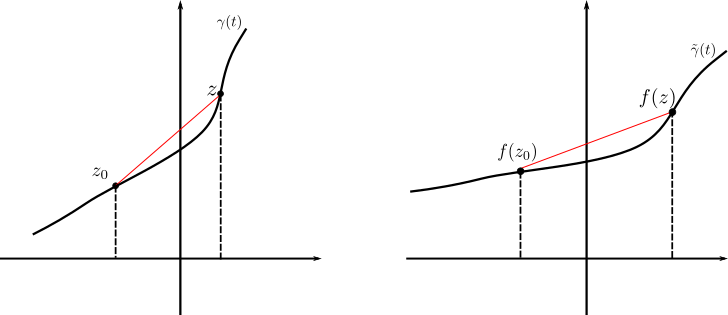
\includegraphics[scale = 1]{geom sense.png}}
	\caption*{Шматок кривої навколо т. $z_0$ розтянули та повернули на деякий кут. (на малюнку масштаб не відповідає реальності: тут $z$ має бути близьким до $z_0$).}
	\end{figure}
	
\begin{example}
Знайти кут повороту та коефіцієнт розтягнення в т. $z_0 = 1+i$ для $f(z) = z^3$.\\
$f(z_0)=(1+i)^3=(-2+2i)$, це нам ще знадобиться.\\
Оскільки $f'(z) = 3z^2$, то $f'(z_0) = 3(1+i)^2 = 6i$
$\displaystyle \implies |f'(z_0)| = 6, \arg f'(z_0) = \frac{\pi}{2}$.
\end{example}
	%END OF PARAGRAPH 2%
	\newpage
	
	
\section{Інтегрування}
\subsection{Основні методи інтегрування}
%GB approach (inaccurate)
\iffalse
Задано функцію $f(z) = u(x,y) + iv(x,y)$. Нехай також $\gamma$ - орієнтований шлях в просторі $\mathbb{C}$. Необхідно знайти такий інтеграл:\\
$\displaystyle \int\displaylimits_{\gamma} f(z)\,dz = \int\displaylimits_{\gamma} \left(u(x,y)+iv(x,y) \right)\,\underset{(?)}{(dx+i\,dy)} \overset{(\textrm{розкриваємо дужки)}}{=} \\ = \int\displaylimits_{\gamma} u(x,y)\,dx-v(x,y)\,dy+ i\int\displaylimits_{\gamma} v(x,y)\,dx+u(x,y)\,dy$.\\
Отже, щоб обчислити інтеграл від комплексної функції $f$ по $\gamma$, треба обчислити стандартний криволінійний інтеграл II роду, що праворуч.\\
\textit{Всі рівності вони є неформальними, але ГБ не хотів витрачати час на строгий вивід.}
\bigskip \\
Якщо $\gamma = \{ z(t), t \in \overrightarrow{[a,b]} \}$ та $dz(t)=z'(t)\,dt$, то інтеграл зведеться до такого вигляду:\\
	$\displaystyle \int\displaylimits_{\gamma} f(z)\,dz = \int_a^b f(z(t))z'(t)\,dt$\\
Або\\
$\displaystyle\int\displaylimits_{\gamma} u(x,y)\,dx-v(x,y)\,dy+ i\int\displaylimits_{\gamma} v(x,y)\,dx+u(x,y)\,dy = \\ = \int_a^b u(x(t),y(t))x'(t)-v(x(t),y(t))y'(t)\,dt + i\int_a^b v(x(t),y(t))x'(t)+u(x(t),y(t))y'(t)\,dt$
	
\begin{example}
Обчислити $\displaystyle\int\displaylimits_{\gamma} \operatorname{Im}(z) \,dz$, де  $\gamma=\{(x,y): y=2x^2, 0 \leq x \leq 1 \}$.\\
	$z=x+iy=x+2ix^2 \Rightarrow dz=dx+i\,dy=(1+4ix)\,dx$\\
Тоді $\displaystyle\int\displaylimits_{\gamma} \operatorname{Im}(z) \,dz = \int_0^1 2x^2(1+4ix)\,dx = \int_0^1 2x^2+8ix^3\,dx = \frac{2}{3}+2i$
\end{example}
\fi

Задано функцію $f: G \to \mathbb{C}$, де $G$ - деяка область. Нехай $\Gamma \subset G$ - кусково-гладка крива орієнтовна крива, що має почааток $z_0$ та кінець $z$.\\
Розіб'ємо криву $\Gamma$ на дуги точками $\tau = \{z_0,z_1,\dots,z_{n-1},z_n\}$, що розташовані послідовно в додатному напрямку кривої. Оберемо $\xi_k$ на кожній дузі між $z_{k-1},z_k$.\\
Позначимо $|\tau| =\displaystyle \max_{k = \overline{1,n}} |z_{k}-z_{k-1}|$.\\
Складемо інтегральну суму $\displaystyle\sum_{k=1}^n f(\xi_k) (z_{k-1}-z_k) = \sigma(f,\tau,\xi)$.
	
\begin{definition}
Число $C \in \mathbb{C}$ називається \textbf{інтегралом} від функції $f$ вздовж кривої $\Gamma$, якщо
\begin{align*}
\forall \varepsilon > 0: \exists \delta > 0: \forall (\tau,\xi): |\tau| < \delta \implies |\sigma(f,\tau,\xi) - C| < \varepsilon
\end{align*}
Позначення: $C = \displaystyle\int\displaylimits_\Gamma f(z)\,dz$.
\end{definition}

\begin{theorem}
Задано функцію $f \in C_{\text{piecewise}}(G)$, де $G$ - область. Нехай $\Gamma \subset G$ - кусково-гладка крива. Розкладемо $f(z) = u(x,y) + iv(x,y)$. Тоді інтеграл від $f$ вздовж кривої $\Gamma$ буде існувати, причому\\
$\displaystyle\int\displaylimits_\Gamma f(z)\,dz = \int\displaylimits_\Gamma u(x,y)\,dx - v(x,y)\,dy + i \int\displaylimits_\Gamma v(x,y)\,dx + u(x,y)\,dy$.
\end{theorem}

\begin{proof}
Маємо $f(z) = u(x,y) + iv(x,y)$, також $z_k = x_k + iy_k$, а також $\xi_k = \tilde{x}_k + i \tilde{y}_k$. Тоді\\
$\sigma(f,\tau,\sigma) = \displaystyle\sum_{k=1}^n f(\xi_k) (z_k-z_{k-1}) = \sum_{k=1}^n (u(\tilde{x}_k,\tilde{y}_k)+iv(\tilde{x}_k,\tilde{y}_k))(x_k-x_{k-1} + i(y_k-y_{k-1})) = \\
= \sum_{k=1}^n (u(\tilde{x}_k, \tilde{y}_k) \Delta x_k - v(\tilde{x}_k, \tilde{y}_k) \Delta y_k ) + i \sum_{k=1}^n (v(\tilde{x}_k, \tilde{y}_k) \Delta x_k + u(\tilde{x}_k, \tilde{y}_k) \Delta y_k )$.\\
Запишу я ось так: $\sigma = \sigma_{Re} + i \sigma_{Im}$.\\
Оскільки функція $f$ кусково неперервна, то тоді функції $u,v$ також. Зокрема векторні поля $(u,-v)^T, (v,u)$ будуть кусково неперервними. Значить, у нас вже існують інтеграли ІІ роду, що знаходяться в теоремі праворуч від знака дорівнює. А тому далі неважко буде прийти до рівності.
\end{proof}

\begin{example}
Обчислити $\displaystyle\int\displaylimits_{\Gamma} \operatorname{Im}(z) \,dz$, де  $\Gamma=\{(x,y): y=2x^2, 0 \leq x \leq 1 \}$.\\
Маємо функцію $f(z) = \Im z$. Запишемо $f(z) = u(x,y) + iv(x,y)$, у цьому випадоку $u(x,y) = y, v(x,y) = 0$. Отже,\\
$\displaystyle\int\displaylimits_{\Gamma} \operatorname{Im}(z) \,dz = \int\displaylimits_{\Gamma} y\,dx + i \int\displaylimits_{\Gamma}y\,dy$.\\
Кожний криволінійний інтеграл II роду обчислимо окремо. Але вже запишу параметризацію:\\
$x = t, t \in [0,1]$, $y = 2t^2$ \hspace{1cm} $dx = dt, dy = 4t\,dt$.\\
$\displaystyle\int\displaylimits_{\Gamma} y\,dx = \int_0^1 2t^2\,dt = \dfrac{2}{3}t^3\Big|_{0}^1 = \dfrac{2}{3}$.\\
$\displaystyle\int\displaylimits_{\Gamma} y\,dy = \int_0^1 2t^2 \cdot 4t\,dt = 2t^4\Big|_{0}^1 = 2$.\\
Отже, остаточно $\displaystyle\int\displaylimits_{\Gamma} \operatorname{Im}(z) \,dz = \dfrac{2}{3} + 2i$.
\end{example}
	
\subsection{Властивості та інші теореми}
\begin{proposition}
Інтеграл $\displaystyle \int\displaylimits_{\gamma} f(z)\,dz$ від параметризації кривої не залежить.\\
\textit{Випливає з властивостей криволінійного інтегралу II роду}
\end{proposition}

\begin{proposition}
Для цього ж інтегралу  виконуються лінійні властивості та адитивність.\\
\textit{Випливають з властивостей криволінійного інтегралу II роду}
\end{proposition}

\begin{theorem}[Ознака модуля]
$\displaystyle \left\lvert\int\displaylimits_{\gamma} f(z)\,dz \right\rvert \leq \int\displaylimits_{\gamma} |f(z)| \,|dz|$
\end{theorem}

\iffalse
%How GB gave the proof (inaccurate one)
\begin{proof}
Параметризуємо криву $\gamma = \{z(t), t \in \vec{[a,b]}\}$. Тоді $z(t)=x(t)+iy(t)$.\\
$dz(t) = (x'(t)+iy'(t))\,dt$\\
$\displaystyle dl = \sqrt{(x'(t))^2+(y'(t))^2}\,dt=|z'(t)|\,dt=|dz|$. Тепер ми знаємо про $|dz|$\\
Позначимо $J = \displaystyle \int\displaylimits_{\gamma} f(z)\,dz$. Оскільки це є комплексне число, то $J = |J|e^{i\varphi} \implies |J|=Je^{-i\varphi}$. Тоді\\
$\displaystyle \abs{\int\displaylimits_{\gamma} f(z)\,dz} = e^{-i \varphi} \int\displaylimits_{\gamma} f(z)\,dz = \int_a^b e^{-i \varphi} f(z(t)) z'(t)\,dt = \\ = \int_a^b \Re(e^{-i \varphi} f(z(t)) z'(t))\,dt + \overbrace{\int_a^b \Im(e^{-i \varphi} f(z(t)) z'(t))\,dt}^{=0} =\int_a^b \Re(e^{-i \varphi} f(z(t)) z'(t))\,dt \\ \overset{|J| \geq 0}{=} \abs{\int_a^b \Re(e^{-i \varphi} f(z(t)) z'(t))\,dt} \leq \int_a^b |\Re(e^{-i \varphi}|f(z(t))||z'(t))|\,dt \boxed{\leq} $\\
Якщо $w = \alpha + i \beta$, то $|w| = \sqrt{\alpha^2 + \beta^2} \geq \sqrt{\alpha^2} = |\Re w|$. Тобто $|\Re w| \leq |w|$.\\
$\boxed{\leq} \displaystyle \int_a^b |e^{-i \varphi} f(z(t)) z'(t)|\,dt = \int_a^b |f(z(t))|z'(t)\,dt = \int\displaylimits_{\gamma} |f(z)|\,|dz|$
\end{proof}
\fi

%Proof based on Riemann's sum
\begin{proof}
$\displaystyle\abs{\displaystyle\sum_{k=1}^n f(\xi_k) (z_{k-1}-z_k)} \leq \sum_{k=1}^n |f(\xi_k) |z_{k-1}-z_k| \leq \sum_{k=1}^n f(\xi_k) |z_{k-1}z_k|$.\\
Тут $|z_{k-1}-z_k| \leq |z_{k-1}z_k|$. Ліворуч - це довжина прямої між цими двома точками, а праворуч - це довжина кривої між цими точками.\\
А далі ми просто робимо $|\tau| \to 0$, тоді буде граничний перехід. Отже,\\
$\displaystyle\abs{\int\displaylimits_\gamma f(z)\,dz} \leq \int_\gamma |f(z)|\,|dz|$.\\
Праворуч - це тіпа криволінійний інтеграл $I$ роду по криві $\gamma$. Тут замість $dl$ я написав $|dz|$, щоб був більш вагомий акцент.
\end{proof}
	
Перед іншими теоремами нагадаю дещо.\\
Є область $D$. Однозв'язним називають ту область $D$, де $\partial D$ (границя області) є зв'язною множиною.
\begin{figure}[h]
	\captionsetup{justification=centering}
	\centerline{
\includegraphics[scale = 0.5]{simply_connected.png}}
	\caption*{Ліворуч - однозв'язна область. Праворуч - вже не є однозв'язною, оскільки вона містить (грубо кажучи) дірки.}
\end{figure}

\begin{theorem}[Теорема Коші]
Задано $D$ - обмежена область, $\partial D$ - кусково-гладка границя та функцію $f$ - аналітична в $D \cup \partial D$.\\
Тоді $\displaystyle\int\displaylimits_{\partial D} f(z)\,dz = 0$.
\end{theorem}

\begin{proof}
$\displaystyle\int\displaylimits_{\partial D} f(z)\,dz = \int\displaylimits_{\partial D} u\,dx-v\,dy + i\int\displaylimits_{\partial D} v\,dx+u\,dy \fbox{=}$\\
За теоремою Коші-Рімана, можна побачити, що коефіцієнти при $dx$ рівні коефіцієнту при $dy$ в кожному інтегралі. Тоді за лемою Пуанкаре про незалежність від шляху, ми отримаємо бажане.\\
$\fbox{=} 0$.
\end{proof}
	
\begin{corollary}
Задано функцію $f$ - аналітична в однозв'язній області $D$. Тоді для довільного замкненого контуру $\gamma$ в $D$ виконується рівність:\\
$\displaystyle\oint\displaylimits_{\gamma} f(z)\,dz=0$.
\begin{figure}[h]
\centerline{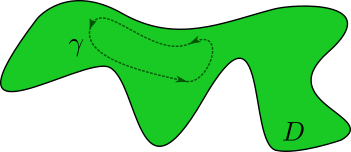
\includegraphics[scale = 1]{g1026.png}}
\caption*{Однозв'язна область $D$ і замкнений контур $\gamma$}
\end{figure}
\end{corollary}

\begin{corollary}
Інтеграл від комплексної функції не залежить від шляху. А тому якщо є якась крива $\gamma$, що проходить через $z_1,z_2$, то ми можемо застосувати позначення:\\
$\displaystyle\int\displaylimits_\gamma f(z)\,dz = \int_{z_1}^{z_2} f(z)\,dz$.
\end{corollary}

\begin{example}
$\displaystyle \oint\displaylimits_{|z| = \frac{1}{2}} \frac{z^2}{z-i}\,dz = 0$\\
Звісно, є неприємна точка $z = i$, але незважаючи на це, в колі $\displaystyle |z|=\frac{1}{2}$ наша функція є аналітичною. Тому теорема Коші спрацьовує.
\end{example}

Перед наступною теоремою, я би хотів швидко обчислити один інтеграл.

\begin{example}
Обчислити $\displaystyle\int\displaylimits_\gamma 1\,d\zeta$, де крива $\gamma$ сполучає точки $z_1$ (початок) та $z_2$ (кінець).\\
Оскільки $f(\zeta) = 1$ - аналітична всюди, тоді не буде залежності від шляху. А тому ми можемо розглянути пряму, що проходить через $z_1,z_2$.\\
$\displaystyle\int\displaylimits_\gamma 1\,d\zeta = \int\displaylimits_\gamma 1 \,dx + i \int\displaylimits_\gamma 1\,dy \boxed{=}$\\
Ми маємо $z_1 = x_1+iy_1$ та $z_2 = x_2+iy_2$. Запишемо параметризацію:\\
$x = t, t \in [x_1,x_2]$ та $y = \dfrac{y_2-y_1}{x_2-x_1}(t-x_1) + y_1$. Тоді звідси $dx = dt, dy = \dfrac{y_2-y_1}{x_2-x_1}\,dt$.\\
$\boxed{=} \displaystyle\int_{x_1}^{x_2}\,dt + i \int_{x_1}^{x_2} \dfrac{y_2-y_1}{x_2-x_1}\,dt = x_2-x_1 + i \dfrac{y_2-y_1}{x_2-x_1}(x_2-x_1) = z_2 - z_1$.\\
Окремо треба розглядати випадок вертикальних та горизонтальних прямих, але все ясно там.\\
Отже, $\displaystyle\int_\gamma 1\,d\zeta = \int_{z_1}^{z_2} 1\,d\zeta = z_2-z_1$ - схоже на застосування формули Ньютона-Лейбніца. У цьому випадку $F(z) = z$ буде первісною для функції $f(z) = 1$.
\end{example}

\begin{theorem}
Задано функцію $f$ - аналітична в однозв'язній області $D$. Тоді функція $f$ має первісну $F$ в області $D$.
\end{theorem}

\begin{proof}
Розглянемо функцію $F(z)=\displaystyle \int_{z_0}^z f(\zeta)\,d\zeta$ - інтеграл з верхньою межею. Перевіримо, що $F'(z)=f(z)$.\\
	$\displaystyle \frac{F(z)-F(z_1)}{z-z_1} = \frac{1}{z-z_1} \left[ \int_{z_0}^z f(\zeta)\,d\zeta - \int_{z_0}^{z_1} f(\zeta)\,d\zeta \right] = \frac{1}{z-z_1} \int_{z_1}^z f(\zeta)\,d\zeta$\\
Водночас за попереднім прикладом, отримаємо\\
	$\displaystyle f(z_1)=f(z_1)\frac{1}{z-z_1}\cdot(z-z_1)=\frac{1}{z-z_1} \int_{z_1}^z f(z_1)\,d\zeta$\\
Звідси випливає, що:\\
$\displaystyle \left\lvert \frac{F(z)-F(z_1)}{z-z_1} - f(z_1) \right\rvert = \frac{1}{|z-z_1|} \left\lvert \int_{z_1}^z f(\zeta)\,d\zeta - \int_{z_1}^z f(z_1)\,d\zeta \right\rvert =\\= \frac{1}{|z-z_1|} \left\lvert \int_{z_1}^z f(\zeta)-f(z_1)\,d\zeta \right\rvert \leq \frac{1}{|z-z_1|} \int_{z_1}^z |f(\zeta)-f(z_1)|\,|d\zeta|\fbox{<}$\\
	Оскільки $f$ - аналітична, то вона є неперервною. Звідси - рівномірно неперервна, тобто $\forall \varepsilon>0$ $\exists \delta: \forall z: |z-z_0|<\delta \Rightarrow |f(z)-f(z_1)|<\varepsilon$. Тоді $|\zeta - z_1|<\delta \Rightarrow |f(\zeta)-f(z_1)|<\varepsilon$\\
	$\displaystyle \fbox{<} \frac{1}{|z-z_1|} \int_{z_1}^z \varepsilon \,|d\zeta| = \varepsilon$\\
	Це означає, що $\displaystyle \exists \lim_{z\to z_1} \frac{F(z)-F(z_1)}{z-z_1}=f(z_1)=F'(z_1)$. І це $\forall z_1 \in D$
\end{proof}
	
\begin{corollary}
Якщо $\textrm{Ф}$ - первісна, то $\displaystyle \int_{z_0}^{z_1} f(z)\,dz = \textrm{Ф}(z_1)-\textrm{Ф}(z_0)$.
\end{corollary}

\begin{proof}
$\textrm{Ф}$ - первісна $\implies \textrm{Ф}'(z)=f(z)$\\
За щойно доведеною теоремою, $F'(z)=f(z)$. Отже, $\textrm{Ф}(z)=F(z)+C$\\
$\begin{cases}
	\textrm{Ф}(z_0) = 0 + C\\
	\textrm{Ф}(z_1) = F(z_1) + C\\
\end{cases} \implies F(z_1)=\textrm{Ф}(z_1)-\textrm{Ф}(z_0)$
\end{proof}

\begin{remark}
Існування первісної не обов'язково в однозв'язній області.
\end{remark}

\subsection*{Трохи ліричного відступу по темі}
У нас взагалі ще існують функції вигляду $f: A \to \mathbb{C}$, де тепер $A \subset \mathbb{R}$. Тобто функція приймає дійсне число, а повертає вже комплексне. Тоді функцію $f$ можна розписати як\\
$f(t) = u(t) + iv(t)$.\\
У цьому випадку $u(t) = \Re f(t), v(t) = \Im f(t)$, обидва $u,v: A \to \mathbb{R}$.
\bigskip \\
Оскільки $\mathbb{R} \subset \mathbb{C}$ (як множини чисел), то зокрема $A \subset \mathbb{C}$, а тому ось цей типаж функції ми можемо розглядати як функцію, що приймає комплексне число, а повертає комплексне значення. Ось так:\\
$u(t) = u(t,s)$, де $s = 0$\\
$v(t) = v(t,s)$, де $s = 0$\\
$f(t) = u(t,s) + iv(t,s) = f(t+is)$, де $s = 0$.
\bigskip \\
Тепер розглянемо функцію $f: A \to \mathbb{C}$, де $A = [a,b] \subset \mathbb{R}$. Наш відрізок $[a,b]$ буде кривою $\gamma$, починаючи з точки $a$. Тоді подивимось на інтеграл:\\
$\displaystyle\int\displaylimits_\gamma f(z)\,dz = \int_\gamma u(x,y)\,dx -v(x,y)\,dy + i \int\displaylimits_\gamma v(x,y)\,dx + u(x,y)\,dy \boxed{=}$\\
Параметризація кривої: $x = t, t \in [a,b], y = 0$. Звідси маємо $dx = dt, dy = 0$.\\
$\boxed{=} \displaystyle\int_a^b u(t,0)\,dt + i \int_a^b v(t,0)\,dt = \int_a^b u(t)\,dt + \int_a^b v(t)\,dt$.\\
Із іншого боку, відрізок $[a,b]$ на комплексній площині буде однов'язною (бо це одна границя, яка зв'язна), тому можна записати так:\\
$\displaystyle\int\displaylimits_\gamma f(z)\,dz = \int_a^b f(z)\,dz = \int_a^b u(t)+iv(t)\,dt$.\\
Таким чином, ми чесно отримали, що
$$ \int_a^b u(t)+iv(t)\,dt = \int_a^b u(t)\,dt + i \int_a^b v(t)\,dt$$
при $u,v$ - дійсно значні функції.
\bigskip \\
\textbf{Повернімось до основної теми}

\begin{theorem}
Задано криву $\gamma$ параметричним рівнянням $z = z(t)$, причому $t \in [\alpha,\beta]$. Тоді\\
$\displaystyle\int\displaylimits_\gamma f(z)\,dz = \int_\alpha^\beta f(z(t)) z'(t)\,dt$.
\end{theorem}

\begin{proof}
Маємо криву $z(t) = x(t) + iy(t)$. Тоді розпишемо, що маємо:\\
$\displaystyle\int\displaylimits_\gamma f(z)\,dz = \int\displaylimits_\gamma u(x(t),y(t))\,dx - v(x(t),y(t))\,dy + i \int\displaylimits_\gamma v(x(t),y(t))\,dx + u(x(t),y(t)\,dy = \\
= \int_{\alpha}^{\beta} u(x(t),y(t))x'(t)-v(x(t),y(t))y'(t)\,dt + i \int_\alpha^\beta v(x(t),y(t))x'(t) + u(x(t),y(t))y'(t)\,dt = \\
= \int_\alpha^\beta [u(x(t),y(t))+iv(x(t),y(t))]x'(t) + [iu(x(t),y(t))-v(x(t),y(t))]y'(t)\,dt = \\
= \int_\alpha^\beta [u(x,y) + iv(x,y)]x'(t) + i[u(x,t) + v(x,y)]y'(t)\,dt = \int_\alpha^\beta f(z(t)) (x'(t)+iy'(t))\,dt = \int_\alpha^\beta f(z(t))z'(t)\,dt$.
\end{proof}

\begin{example}[Важливий]
Обчислити $\displaystyle \oint\displaylimits_{C} \frac{dz}{(z-z_0)^n}$ по колу $C = \{z: |z-z_0|=R\}, n\in \mathbb{N}$.\\
	Зробимо параметризацію: $\displaystyle z-z_0=Re^{it},t \in \overrightarrow{[0,2\pi]}$\\
	$dz=Rie^{it}\,dt$\\
	$\implies \displaystyle \oint \frac{dz}{(z-z_0)^n}= \int_0^{2\pi} \frac{Rie^{it}\,dt}{R^ne^{nit}}=i\int_0^{2\pi} R^{1-n} e^{(1-n)it}\,dt =$
	$\left[ 
      \begin{gathered} 
        2 \pi i, n =1 \\ 
        \frac{1}{R^{n-1}}\frac{1}{(1-n)i}e^{(1-n)it} \Big|_0^{2\pi} = 0, n \neq 1 \\ 
      \end{gathered} 
\right.$.\\
По-перше, зауважимо, що при $n = 1$ інтеграл ніяк не залежить від радіусу кола, а також від центру кола $z_0$.\\
По-друге, цей приклад гарантує, що умова однозв'язності області важлива для теореми Коші. У цьому випадку область, що всередині кривої $C$ без точки $z_0$, не буде однозв'язною.
\end{example}

\begin{theorem}[Теорема Коші 2]
Задано функцію $f$ - аналітична в області $D$. Відомо, що замкнені контури $\gamma_1$, $\gamma_2$ обмежують однозв'язну область $D_{\gamma_1 \gamma_2}$, де $f$ - аналітична. Тоді
	\begin{align*}
	\oint\displaylimits_{\gamma_1} f(z)\,dz = \oint\displaylimits_{\gamma_2} f(z)\,dz
	\end{align*}
\begin{figure}[h]
	\centerline{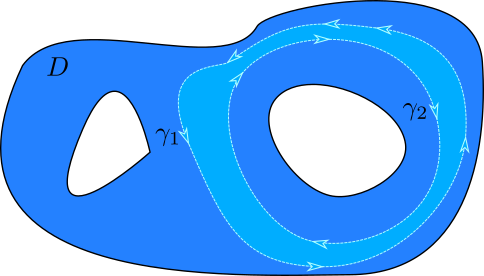
\includegraphics[scale = 1]{path1375.png}}
	\caption*{Тут $D_{\gamma_1 \gamma_2}$ яскраво-блакитна область}
\end{figure}
\end{theorem}

\begin{proof}
Вважатимемо, що контури $\gamma_1^+,\gamma_2^+$ протилежно напрямлені.\\
	$\displaystyle\oint\displaylimits_{\gamma_1^+} f(z)\,dz - \oint\displaylimits_{\gamma_2^+} f(z)\,dz = \displaystyle\oint\displaylimits_{\gamma_1^+} f(z)\,dz + \oint\displaylimits_{\gamma_2^-} f(z)\,dz = \oint\displaylimits_{\gamma_1^+ \cup \gamma_2^-} f(z)\,dz = \\ = \oint\displaylimits_{\gamma_1^+ \cup \gamma_2^-} u\,dx-v\,dy + i\oint\displaylimits_{\gamma_1^+ \cup \gamma_2^-} u\,dy+v\,dx \overset{\textrm{ф-ла Гріна}}{=} \\ = \iint\displaylimits_{D_{\gamma_1^+ \cup \gamma_2^-}} -\frac{\partial v}{\partial x} - \frac{\partial u}{\partial y} \,dxdy + i\iint\displaylimits_{D_{\gamma_1^+ \cup \gamma_2^-}} -\frac{\partial v}{\partial y} + \frac{\partial u}{\partial x} \,dxdy \overset{\textrm{умова Коші-Рімана}}{=} 0$
\end{proof}

\begin{theorem}[Інтегральна формула Коші]
Задано функцію $f$ - аналітична в області $D$ і т. $z_0 \in D$. Відомо, що замкнений контур $\gamma \in D$ охоплює т. $z_0$ та обмежує однозв'язну область $D_{\gamma}$. \\
Тоді $\displaystyle\oint\displaylimits_{\gamma} \frac{f(z)}{z-z_0}\,dz = 2 \pi i \cdot f(z_0)$.
	\begin{figure}[h]
	\centerline{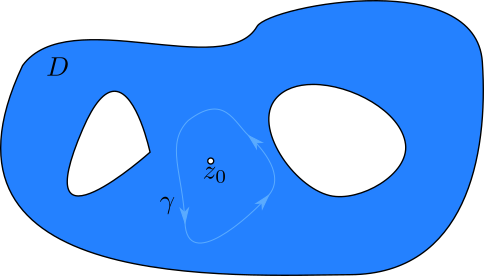
\includegraphics[scale = 1]{path1376.png}}
	\caption{Контур $\gamma$ утворює однозв'язну область.}
	\end{figure}
\end{theorem}
	
\begin{proof}
Розглянемо коло $C = \{ z: |z-z_0|=\rho\}$ таке, що $C \subset D_{\gamma}$. Тоді за попередньою теоремою,\\
	$\displaystyle\oint\displaylimits_{\gamma} \frac{f(z)}{z-z_0}\,dz = \oint\displaylimits_C \frac{f(z)}{z-z_0}\,dz \boxed{=}$\\
	Покладемо $z-z_0=\rho e^{it} \implies dz=\rho ie^{it}\,dt$\\
	$\displaystyle \boxed{=} \int_{0}^{2\pi} \frac{f(z_0+\rho e^{it})}{\rho e^{it}} \cdot \rho i e^{it} \,dt = i \int_{0}^{2\pi} f(z_0+ \rho e^{it})\,dt = i \int_0^{2\pi} f(z_0+ \rho e^{it}) - f(z_0)\,dt + i \int_0^{2\pi} f(z_0)\,dt = \\
	= i \int_0^{2\pi} f(z_0+ \rho e^{it}) - f(z_0)\,dt + 2\pi i f(z_0)$.\\
	А далі зауважимо, що $\displaystyle\int_0^{2\pi} f(z_0+\rho e^{it})\,dt \to 0$ при $\rho \to 0$ в силу того, що $f$ аналітична. Тому легко отримаємо бажану рівність.
\end{proof}

\begin{example}
$\displaystyle\oint\displaylimits_{|z|=1} \frac{\sin z}{z} \,dz = 2\pi i \sin 0 = 0$.
\end{example}

\subsection*{Більш просунуті речі}
\begin{definition}
\textbf{Первісною} функції $f$ в області $D$ назвемо таку голоморфну в $D$ функцію $F$, що $$ F'(z) = f(z)$$
\end{definition}

\begin{theorem}
Маємо функцію $f$ в області $D$. Нехай $F,\Phi$ - дві первісні в області $D$.\\
Тоді $\Phi(z) = F(z) + C$.\\
\textit{Зрозуміло.}
\end{theorem}

\begin{lemma}
Задано функцію $f \in C(U)$, де $U = \{z: |z-a| < r\}$ - коло. Візьмемо $\Delta \subset U$ - будь-який трикутник, одна з вершин це точка $a$, причому границі лежать також всередині. Відомо, що $\displaystyle\oint_{\partial \Delta} f(z)\,dz = 0$.\\
Тоді існує первісна $F(z) = \displaystyle\int_a^z f(\zeta)\,d\zeta$ в області $U$.
\end{lemma}

\begin{proof}
\begin{figure}[H]
\centering
\begin{tikzpicture}
\draw[dashed] (0,0) circle (2) node at (-2,-1) {$U$};
node at (0,-0.2) {$a$};
\draw[->] (0,0) -- (1.4,1) -- (0.5,1.5) -- cycle;
\node at (1.4,0.8) {$z$};
\node at (0.5,1.7) {$z+h$};
\end{tikzpicture}
\end{figure}
Оберемо довільну точку $z \in U$, беремо таке $h$, щоб $z+h \in U$. Тоді\\
$\displaystyle\int_a^z f(\zeta)\,d\zeta + \int_z^{z+h} f(\zeta)\,d\zeta = \int_a^{z+h} f(\zeta)\,d\zeta$.\\
Дана рівність виконана в силу того, що $\displaystyle\oint_{\partial \Delta} f(z)\,dz = 0$.\\
$F(z+h)-F(z) = \displaystyle\int_z^{z+h}f(\zeta)\,d\zeta$.\\
Також зауважимо, що $\displaystyle\int_z^{z+h} f(z)\,d\zeta = f(z)h$, а тому звідси\\
$\abs{\dfrac{F(z+h)-F(z)}{h}-f(z)} \leq \dfrac{1}{|h|} \displaystyle\int_z^{z+h} |f(\zeta) - f(z)|\,d\zeta < \varepsilon$.\\
Оскільки $f \in C(U)$, то тоді $\forall \varepsilon > 0: \exists \delta: \forall \zeta: |\zeta-z| < \delta \implies |f(\zeta)-f(z)| < \varepsilon$.\\
Таким чином, $F'(z) = f(z)$ в будь-якій точці $z \in U$.
\end{proof}

\begin{remark}
Не обов'язково вимагати, щоб саме будь-який трикутник мав інтеграл нулевий. Адже цей трикутник можна розписати як суму трьох трикутників з вершиною $a$, а всі вони нулі автоматом.
\end{remark}

\begin{lemma}
Задано функцію $f$ - голоморфна в області $D$.\\
Тоді для будь-якого трикутника, $\Delta \subset D$ разом з границями маємо $\displaystyle\oint_{\partial \Delta} f(z)\,dz = 0$.
\end{lemma}

\begin{proof}
!Припустимо, що існує трикутник $\Delta \subset D$ разом з границями, для якого $\displaystyle\abs{ \oint_{\partial \Delta} f(z)\,dz} = M > 0$.\\
Трикутник $\Delta$ розіб'ємо на $4$ трикутника, проводячи середні лінії.
\begin{figure}[H]
\centering
\begin{tikzpicture}
\draw (0,0)--(3,0)--(1.5,1.5)--cycle;
\draw (1.5,0)--(2.25,0.75)--(0.75,0.75)--cycle;
\end{tikzpicture}
\end{figure}
Будемо всі трикутники орієнтовувати в протилежний напрямок.\\
$\displaystyle\oint_{\partial \Delta} f(z)\,dz = \oint_{\partial \Delta_{(1)}} f(z)\,dz + \oint_{\partial \Delta_{(2)}} f(z)\,dz + \oint_{\partial \Delta_{(3)}} f(z)\,dz + \oint_{\partial \Delta_{(4)}} f(z)\,dz$.\\
Думаю, цю рівність пояснювати не треба. Звідси випливає, що серед чотирьох трикутників існує один, який я позначу $\Delta_1$, для якого\\
$\displaystyle\abs{\oint_{\partial \Delta_1} f(z)\,dz} \geq \dfrac{M}{4}$.\\
Ось цей трикутник $\Delta_1$ ми аналогічно розбиваємо, проводячи середнії лінії. Аналогічно записуємо інтеграл за $\partial \Delta_1$ як суму інтегралів по кожному трикутнику. Аналогічно знайдеться серед чотирьох трикутників трикутник, який позначу за $\Delta_2$, для якого\\
$\displaystyle\abs{\oint_{\partial \Delta_1} f(z)\,dz} \geq \dfrac{M}{4^2}$.\\
\vdots \\
Так продовжуємо, отримаємо $\displaystyle\abs{\oint_{\partial \Delta_n} f(z)\,dz} \geq \dfrac{M}{4^n}, \forall n \geq 1$.\\
Ці трикутники $\Delta_n$ зобов'язані мати спільну точку $z_0 \in \Delta \subset D$. У силу голоморфності функції $f$, маємо в т. $z_0$, що\\
$\forall \varepsilon > 0: \exists \delta: \forall z \in U': \abs{\alpha(z)} = \abs{ \dfrac{f(z)-f(z_0)}{z-z_0} - f'(z_0) } < \varepsilon$.\\
У цьому випадку $U' = \{z: 0<|z-z_0|<\delta\}$. Цей окіл має містити якийсь трикутник, що бере участь у послідовності $\Delta_1,\Delta_2,\dots$. Позначу за $\Delta_N$. Отже,\\
$\displaystyle\oint_{\partial \Delta_N} f(z)\,dz = \oint_{\partial \Delta_N} f(z_0)\,dz + \oint_{\partial \Delta_N} f'(z_0)(z-z_0)\,dz + \oint_{\partial \Delta_N} \alpha(z)(z-z_0)\,dz = \oint_{\partial \Delta_N} \alpha(z)(z-z_0)\,dz$.\\
Зауважимо, що $|z-z_0| \leq |\partial \Delta_N|$, де $|\partial \Delta_N|$ позначаю за периметр трикутника. Причому за нашою побудовою, $|\partial \Delta_N| = \dfrac{|\partial \Delta|}{2^N}$. Отже,\\
$\displaystyle\abs{\oint_{\partial \Delta_N} f(z)\,dz} = \abs{\oint_{\partial \Delta_N}} \alpha(z)(z-z_0)\,dz < \varepsilon |\partial \Delta_N|^2 = \varepsilon \dfrac{|\partial \Delta|^2}{4^N}$.\\
Використовуючи найпершу нерівність разом з найостаннішою, отримаємо $0 \leq M < \varepsilon |\partial \Delta|^2 \implies M =0$. Суперечність!
\end{proof}

\begin{theorem}[Існування первісної локально]
Задано функцію $f$ - голоморфна в області $D$.\\
Тоді для будь-якого кола $U = \{z: |z-z_0| < r\} \subset D$ існує первісна $F(z) = \displaystyle\int_{z_0}^z f(\xi)\,d\xi$.\\
\textit{Спочатку друга лема, потім перша лема.}
\end{theorem}
	
\subsection{Степеневі ряди}
Для комплексних чисел степеневий ряд визначається так само:
\begin{align*}
	\sum_{n=0}^{\infty} c_n(z-z_0)^n
\end{align*}
Так само радіус збіжності визначається або за Даламбером, або за Коші-Адамаром.
	$$R = \displaystyle\lim_{n \to \infty}\frac{|c_n|}{|c_{n+1}|} \text{ або } R = \displaystyle\frac{1}{\displaystyle\uplim_{n \to \infty} \sqrt[n]{|c_n|}}$$
Область збіжності визначає нерівність: $$|z-z_0|<R$$

\begin{example}
Визначити область збіжності ряду $\displaystyle \sum_{n=1}^{\infty} \frac{(z-1)^n}{n^2 2^n}$.\\
Знайдемо радіус $R$ за Коші-Адамара:\\
$R = \displaystyle\frac{1}{\displaystyle\uplim_{n \to \infty} \sqrt[n]{\frac{1}{|n^2 2^n|}}} = \frac{1}{\displaystyle \frac{1}{2} \lim_{n \to \infty} \sqrt[n]{\frac{1}{|n^2|}} } = 2$\\
Отже, степеневий ряд збігається, коли $|z-1|<2$.
\end{example}

Надалі будемо вважати, що ми вже знаємо про цей факт: $$\displaystyle \sum_{z=0}^{\infty} z^n = \frac{1}{1-z} \text{ при } |z|<1$$
Хоча це доволі неважко показати, але тим не менш.

\begin{theorem}[Теорема Тейлора]
Задано функцію $f$ - аналітична в області $D$.\\ Тоді знайдеться коло $\{\zeta: |\zeta-z_0|<R\} \subset D$, де функція $f$ розкладається в ряд
\begin{align*}
	f(z) = \sum_{n=0}^{\infty} c_n(z-z_0)^n \\
	c_n = \frac{1}{2\pi i} \oint\displaylimits_{|\zeta-z_0|=\rho<R} \frac{f(\zeta)}{(\zeta-z_0)^{n+1}}\,d\zeta
\end{align*}
\end{theorem}

\begin{proof}
Скористаємось інтегральною формулою Коші:
	$\displaystyle \oint\displaylimits_{\gamma} \frac{f(\zeta)}{\zeta-z}\,d\zeta = 2\pi i f(z)$\\
	За ще одною теоремою Коші, ми можемо змінити контуру інтегрування. Тоді отримаємо:\\
	$f(z) = \displaystyle \frac{1}{2\pi i} \oint\displaylimits_{|\zeta-z_0|=\rho} \frac{f(\zeta)}{\zeta-z}\,d\zeta = \frac{1}{2\pi i}\oint\displaylimits_{|\zeta-z_0|=\rho} \frac{f(\zeta)}{\zeta-z_0+z_0-z}\,d\zeta \boxed{=}$\\
	Тут ми оберемо таке $\rho$, щоб $\displaystyle \abs{\frac{z-z_0}{\zeta - z_0}}<1$\\
	$\boxed{=} \displaystyle \frac{1}{2\pi i} \oint\displaylimits_{|\zeta-z_0|=\rho} \frac{f(\zeta)}{\zeta-z_0} \cdot \frac{1}{\displaystyle 1- \frac{z-z_0}{\zeta -z_0}} \,d\zeta = \frac{1}{2\pi i}\oint\displaylimits_{|\zeta-z_0|=\rho} \frac{f(\zeta)}{\zeta-z_0} \cdot \sum_{n=0}^{\infty} \frac{(z-z_0)^n}{(\zeta-z_0)^n} \,d\zeta = \\ = \sum_{n=0}^{\infty}\frac{1}{2\pi i} \oint\displaylimits_{|\zeta-z_0|=\rho} \frac{f(\zeta)}{(\zeta-z_0)^{n+1}} \,d\zeta \cdot (z-z_0)^n$\\
	Нарешті, якщо покласти $c_n = \displaystyle\frac{1}{2\pi i}\oint\displaylimits_{|\zeta-z_0|=\rho} \frac{f(\zeta)}{(\zeta-z_0)^{n+1}} \,d\zeta$, то $f(z) = \displaystyle\sum_{n=0}^{\infty} c_n(z-z_0)^n$.\\
	Ми внесли інтеграл в середину степеневого ряду. Це також можливо, як в степеневих рядах дійсного аналізу.
\end{proof}

\begin{corollary}
$\displaystyle |c_n| \leq \frac{M}{\rho^n}$, де $\displaystyle M=\max_{z\in D} |f(z)|$.
\end{corollary}

\begin{proof}
	 $\displaystyle |c_n| = \abs{\frac{1}{2\pi i}} \abs{\oint\displaylimits_{|\zeta-z_0|=\rho} \frac{f(\zeta)}{(\zeta-z_0)^{n+1}}\,d\zeta} \leq \frac{1}{2\pi} \oint\displaylimits_{|\zeta-z_0|=\rho} \abs{\frac{f(\zeta)}{(\zeta-z_0)^{n+1}}}\,\abs{dz} \overset{\zeta-z_0= \rho e^{it}}{\leq} \\ \overset{|f(\zeta)| \leq M}{\leq} \frac{1}{2\pi} \int_{0}^{2 \pi} \frac{M}{\rho^n}\,dt = \frac{M}{\rho^n}$
\end{proof}

\begin{theorem}[Теорема Луівілля]
Задано функцію $f$ - аналітична всюди, але обмежена. Тоді $f(z)=C, C \in \mathbb{C}$.
\end{theorem}

\begin{proof}
За попередньою теоремою, ми можемо розкласти в ряд $f(z)$. Оскільки вона всюди аналітична, ми можемо спрямувати $R \to \infty$. Тоді за щойно доведеним наслідком, $\displaystyle |c_n| \leq \frac{M}{R^n} \rightarrow 0$, але $c_n$ ніяк не залежить від обраного $R$.\\
Отже, $c_n=0$ при $n \neq 0 \implies f(z)=c_0$.
\end{proof}

\begin{corollary}
$\cos z$ та $\sin z$ не є обмеженими.
\end{corollary}

\begin{theorem}
Розклад степеневого ряду є єдиним.\\
\textit{Це випливає, насправді, з теореми Тейлора. Можна спробувати припустити, що є два ряди, рівні за значенням, але коефіцієнти різні. Причому, радіус збіжності теж може бути різним. Але розписуючи коефіцієнти, ми прийдемо до їхньої рівності через всілякі теореми Коші.}
\end{theorem}

\begin{proposition}
Задано функцію $f$, що має первісну в області $D$, Тоді $f$ аналітична в $D$.
\end{proposition}

\begin{proof}
Отже, нехай є первісна $F$, яка може розкластися в ряд Тейлора:\\
$\displaystyle F(z)=\sum_{n=0}^{\infty} c_n(z-z_0)^n$,$|z-z_0|<R$. Тоді\\ $\displaystyle f(z)=F'(z)=\sum_{n=1}^{\infty} nc_n(z-z_0)^{n-1} \implies f'(z) = \sum_{n=2}^{\infty} n(n-1)c_n(z-z_0)^{n-2}$\\
Ряд має такий самий радіус збіжності.
\end{proof}

\begin{proposition}
Задано функцію $f$ - аналітична в області $D$. Тоді $f$ - $\infty$-диференційована.
\end{proposition}

\begin{proof}
$\displaystyle f(z)=\sum_{n=0}^{\infty} c_n(z-z_0)^n \implies \\ \forall k\geq1: \exists f^{(k)}(z) = \sum_{n=k}^{\infty} n(n-1) \cdots (n-(k-1))c_n(z-z_0)^{n-k}$. \\
У всіх такий самий радіус збіжності.
\end{proof}

\begin{theorem}
Задані $f,g$ - аналітичні в колі $|z-z_0|<R$ таким чином, що множина $S=\{z: f(z)=g(z)\}$ містить граничну точку $z_0$. Тоді $f(z)=g(z)$ на всьому колі.
\end{theorem}

\begin{proof}
Розкладемо обидві функції в степеневий ряд:\\
	$\displaystyle f(z)=\sum_{n=0}^{\infty} c_n(z-z_0)^n$\\
	$\displaystyle g(z)=\sum_{n=0}^{\infty} a_n(z-z_0)^n$\\
	Далі розглянемо послідовність $\{z_k, k\geq 1\} \subset S$ таку, що $\displaystyle\lim_{k\to\infty} z_k = z_0$. Тоді $\forall k: f(z_k)=g(z_k) \implies \stackbelow{\displaystyle\lim_{k\to\infty} f(z_k)}{c_0} = \stackbelow{\displaystyle\lim_{k\to\infty} g(z_k)}{a_0}$\\
	$f(z_k)-c_0=f(z_k)-a_0$\\
	Ділимо на $z-z_k$. Тоді\\
	$\displaystyle \frac{1}{z_k-z_0}(f(z_k)-c_0) = \frac{1}{z_k-z_0}(f(z_k)-a_0)$\\
	$\displaystyle \sum_{n=1}^{\infty} c_n(z_k-z_0)^{n-1} = \sum_{n=1}^{\infty} a_n(z_k-z_0)^{n-1}$\\
	$\implies c_1 = a_1$ при $k\to\infty$\\
	$f(z_k)-c_0-c_1(z-z_0) = g(z_k)-a_0-a_1(z-z_0)$\\
	Ділимо на $(z-z_k)^2$. Тоді...\\
	За МІ, ми отримаємо, що $\forall n \geq 1: c_n = a_n \Rightarrow f(z)=g(z)$.
\end{proof}

\begin{corollary}
Маємо такі ряди:
\begin{align*}
e^z = \sum_{n=0}^{\infty} \frac{z^n}{n!}\\
\sin z = \sum_{n=0}^{\infty} (-1)^n \frac{z^{2n+1}}{(2n+1)!}\\
\cos z = \sum_{n=0}^{\infty} (-1)^n \frac{z^{2n}}{(2n)!}
\end{align*}
Радіус збіжності - всюди.
\end{corollary}

\begin{proof}
Доведу лише перший ряд. Решта аналогічно.\\
Маємо $f(z) = e^z, g(z)=\displaystyle \sum_{n=0}^{\infty} \frac{z^n}{n!}$.\\
Якщо покласти $S=\mathbb{R}$, то тоді вона має $0$ - гранична точка $S$ та $f(x)=g(x), \forall x \in \mathbb{R}$.\\
	Отже, $f(z)=g(z)$.
\end{proof}

\begin{corollary}
Задано функцію $f$ - аналітична в $D$. Тоді функцію можна розкласти як ряд Тейлора:
\begin{align*}
	f(z) = \sum_{n=0}^{\infty} \frac{f^{(n)}(z_0)}{n!} (z-z_0)^n
\end{align*}
\end{corollary}

\begin{proof}
$f(x)=\displaystyle \sum_{n=0}^{\infty} \frac{f^{(n)}(x_0)}{n!} (x-x_0)^n, |x-x_0|<R$\\ $\displaystyle g(z)=\sum_{n=0}^{\infty} \frac{f^{(n)}(x_0)}{n!} (z-x_0)^n$\\
	Якщо покласти $S=(x_0-R, x_0+R)$, де $x_0$ - гранична точка, то отримаємо $f(z)=g(z)$. 
\end{proof}

\begin{corollary}[Узагальнена інтегральна формула Коші]
Задано функцію $f$ - аналітична в області $D$ і т. $z_0 \in D$. Відомо, що замкнений контур $\gamma \in D$ охоплює т. $z_0$ та обмежує однозв'язну область $D_{\gamma}$. \\
Тоді $\displaystyle\oint\displaylimits_{\gamma} \frac{f(z)}{(z-z_0)^{n+1}}\,dz = \frac{2 \pi i}{n!} f^{(n)}(z_0)$.
\end{corollary}

\begin{example}
Розкласти функцію $\displaystyle \frac{1}{5+z^2}$ в ряд Тейлора\\
	$\displaystyle \frac{1}{5+z^2} = \frac{1}{5} \frac{1}{1 + \frac{z^2}{5}} \overset{\textstyle \frac{z^2}{5} = t}{=} \frac{1}{5} \frac{1}{1+t} = \frac{1}{5} \frac{1}{1-(-t)} = \frac{1}{5} \sum_{n=0}^{\infty} (-t)^n = \sum_{n=0}^{\infty} (-1)^n \frac{z^{2n}}{5^{n+1}}$\\
	Де $\displaystyle |-t|<1 \Rightarrow \abs{\frac{z^2}{5}} < 1 \Rightarrow |z| < \sqrt{5}$
\end{example}

\begin{example}
$\displaystyle \oint\displaylimits_{|z+i|=1} \frac{\sin z}{(z+i)^3} \,dz = \frac{2\pi i}{2!} (\sin z)'' \Big|_{z=-i} = -\pi \sh 1$
\end{example}

\begin{theorem}[Теорема Морери]
Задано функцію $f \in C(D)$, де $D$ - однозв'язна область. Відомо, що для довільного закмненого контуру $\gamma$ в $D$ виконується $\displaystyle \oint\displaylimits_\gamma f(z)\,dz=0$. \\
Тоді $f$ - аналітична в $D$.
\end{theorem}

\begin{proof}
Із умови випливає, що інтеграл не залежить від шляху. Отже, коректно визначеним буде наступний інтеграл:\\
	$\displaystyle F(z)=\int_{z_0}^z f(\zeta)\,d\zeta, z_0 \in D$. Доведемо, що $F$ - первісна до $f$.\\
	$\displaystyle \frac{F(z_0+\Delta z)-F(z_0)}{\Delta z} = \frac{1}{\Delta z} \int_{z_0}^{z_0+\Delta z} f(\zeta) \,d\zeta$\\
	Крім того, $\displaystyle \int_{z_0}^{z_0+\Delta z} f(z_0) \,d\zeta = f(z_0) \Delta z$. Тоді\\
	$\displaystyle \abs{\frac{F(z_0+\Delta z)-F(z_0)}{\Delta z} - f(z_0)} \leq \frac{1}{\abs{\Delta z}} \int_{z_0}^{z_0+\Delta z} \abs{f(\zeta) - f(z)} \,d\zeta \boxed{<}$\\
	Оскільки $f \in C(D)$, то тоді вона неперервна в якомусь колі $\{z: |z-\zeta| >r\} \subset D$. Звідси вона рівномірно неперервна в колі, а далі можна аналогічно (як було на кілька теорем вище) прийти до нерівності $|f(\zeta) - f(z)|<\varepsilon$.\\
	$\boxed{<} \varepsilon$.\\
	Отже, $F'(z) = f(z)$. Тому $F$ - аналітична, а тоді - $\infty$-диференційована. Випливає, що $\exists F''(z)=f'(z) \implies f$ - аналітична.
\end{proof}

\begin{theorem}[Узагальнення]
Задано функцію $f \in C(D)$, де $D$ - однозв'язна область. Тоді наступні умови є еквівалентними:
	\begin{align*}
	\underbrace{\begin{cases}
		\displaystyle\frac{\partial u}{\partial x} = \frac{\partial v}{\partial y}\\
		\displaystyle\frac{\partial u}{\partial y} = -\frac{\partial v}{\partial x}\\
	\end{cases}}_{R}
	 \iff \forall \gamma \subset D: \underbrace{\oint\displaylimits_{\gamma} f(z)\,dz=0}_{C} \iff f \underbrace{\textrm{- розкладається в Тейлора}}_{W}
	\end{align*}
\end{theorem}

\begin{proof}
\begin{figure}[h]
	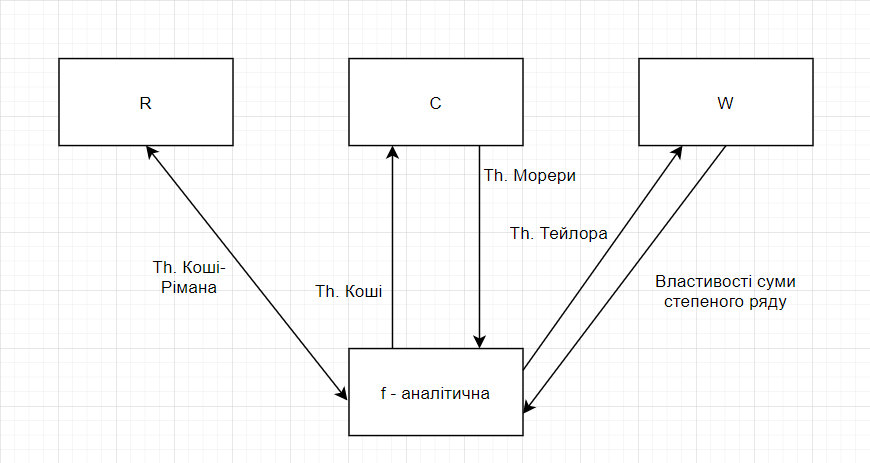
\includegraphics[scale = 0.7]{Pic.png}
	\caption*{Схематичне доведення}
\end{figure}
\end{proof}
	
\subsection{Нулі аналітичної функції}
\begin{definition}
Задано функцію $f$ - аналітична в $D$.\\
Точка $z_0 \in D$ називається \textbf{нулем функції} $f(z)$, якщо $$f(z_0) = 0$$
Точка $z_0 \in D$ називається \textbf{нулем кратності} $k$, якщо $$\exists g -  \text{ аналітична в } D: f(z)=(z-z_0)^k g(z), g(z_0) \neq 0$$
\end{definition}

\begin{theorem}
Задано функція $f$ - аналітична в $D$.\\
$z_0$ - корінь кратності $k \iff \begin{cases} f(z_0)=f'(z_0)=\cdots=f^{(k-1)}(z_0) = 0\\
f^{(k)}(z_0) \neq 0
\end{cases}$.
\end{theorem}

\begin{proof}
	$\boxed{\Rightarrow}$ Дано: $z_0$ - корінь кратності $k$, тобто $\exists g$ - аналітична: $f(z)=(z-z_0)^k g(z)$, $g(z_0) \neq 0$.\\
	Оскільки $g$ - аналітична, то $\displaystyle g(z) = \sum_{n=0}^{\infty} \frac{g^{(n)}(z_0)}{n!} (z-z_0)^n$.\\
	$\implies \displaystyle f(z) = \sum_{n=0}^{\infty} \frac{g^{(n)}(z_0)}{n!} (z-z_0)^{n+k} = \sum_{m=0}^{\infty} \frac{f^{(m)}(z_0)}{m!} (z-z_0)^{m}$.\\
	Ліворуч вираз починається з дужки номера $k$. А правий вираз - з дужки номера $0$. Тому всі вирази з дужками від $0$ до $k-1$ мають бути нулевими. Отже,\\
	$\begin{cases} 
	f(z_0)=f'(z_0)=\cdots=f^{(k-1)}(z_0) = 0\\
	f^{(k)}(z_0) \neq 0
	\end{cases}$
	\hugespace
	$\boxed{\Leftarrow}$ Дано: $\begin{cases} 
	f(z_0)=f'(z_0)=\cdots=f^{(k-1)}(z_0) = 0\\
	f^{(k)}(z_0) \neq 0
	\end{cases}$\\
	$\implies \displaystyle f(z) = \sum_{n=k}^{\infty} \frac{f^{(n)}(z_0)}{n!} (z-z_0)^{n}= (z-z_0)^{k} \sum_{n=k}^{\infty} \frac{f^{(n)}(z_0)}{n!} (z-z_0)^{n-k}$.\\
	Покладемо $\displaystyle g(z) = \sum_{n=k}^{\infty} \frac{f^{(n)}(z_0)}{n!} (z-z_0)^{n-k}$, причому $g(z_0) \neq 0$. Тоді $f(z)=(z-z_0)^k g(z) \\ \implies z_0$ - корінь кратності $k$.
\end{proof}
	
\subsection{Ряди Лорана}
Ряд Лорана має ось такий вигляд:
\begin{align*}
	\sum_{n=-\infty}^{+\infty} c_n(z-z_0)^n
\end{align*}
Розпишемо даний ряд іншим чином:\\
	$\displaystyle \sum_{n=-\infty}^{+\infty} c_n(z-z_0)^n = \sum_{n=-\infty}^{-1} c_n(z-z_0)^n + \sum_{n=0}^{+\infty} c_n(z-z_0)^n \boxed{=}$\\
В першій сумі замінимо лічильник: $n=-k$\\
	$\displaystyle \boxed{=} \underbrace{\sum_{k=1}^{\infty} \frac{c_{-k}}{(z-z_0)^k}}_{\textrm{головна частина}} + \underbrace{\sum_{n=0}^{+\infty} c_n(z-z_0)^n}_{\textrm{правильнаа частина}}$.\\
Далі дізнаємось область збіжності для двох рядів:\\
	- правильна частина: $R = \displaystyle\frac{1}{\displaystyle\uplim_{n \to \infty} \sqrt[n]{|c_n|}} \implies |z-z_0|<R$.\\
	- головна частина: тимчасова заміна $\displaystyle t=\frac{1}{z-z_0}$. Тоді отримаємо степеневий ряд вигляду $\displaystyle \sum_{k=1}^{\infty} c_{-k}t^k$.\\
	$R' = \displaystyle\frac{1}{\displaystyle\uplim_{k \to \infty} \sqrt[k]{|c_{-k}|}} \Rightarrow |t|<R' \implies |z-z_0|>\frac{1}{R'} \overset{\textrm{покладемо}}{=} r$.\\
Таким чином область збіжності ряду Лорану визначається кільцем:
\begin{align*}
	\uplim_{k \to \infty} \sqrt[k]{|c_{-k}|}=r<|z-z_0|<R=\frac{1}{\displaystyle\uplim_{n \to \infty} \sqrt[n]{|c_n|}}
\end{align*}
Ба більше, сума ряду Лорана є аналітичною в цьому кільці.

\begin{theorem}[Теорема Лорана]
Задано функцію $f$ - аналітична в кільці $K=\{z: r<|z-z_0|<R\}$. Тоді $f$ розкладається в ряд Лорана:
	\begin{align*}
	f(z)= \sum_{k=1}^{\infty}\frac{c_{-k}}{(z-z_0)^k}  + \sum_{n=0}^{\infty} c_n(z-z_0)^n\\
	c_m = \frac{1}{2 \pi i}\oint\displaylimits_{|\zeta-z_0|=\rho} \frac{f(\zeta)}{(\zeta-z_0)^{m+1}} \,d\zeta, \textrm{ } r<\rho<R
	\end{align*}
\end{theorem}

\begin{proof}
Скористаємось інтегральною формулою Коші:
	$\displaystyle \oint\displaylimits_{\gamma} \frac{f(\zeta)}{\zeta-z}\,d\zeta = 2\pi i f(z)$.\\
	За ще одною теоремою Коші, ми можемо змінити контуру інтегрування. Тоді отримаємо:\\
	$f(z) = \displaystyle \frac{1}{2\pi i} \oint\displaylimits_{c} \frac{f(\zeta)}{\zeta-z}\,d\zeta \boxed{=}$\\
	Тут $c = c_1 \cup c_2^- = \{\zeta: |\zeta-z_0|<R\} \cup \{\zeta: |\zeta-z_0|>r\}$\\
	 $ \boxed{=} \displaystyle\frac{1}{2\pi i}\oint\displaylimits_{c_1 \cup c_2^-} \frac{f(\zeta)}{\zeta-z}\,d\zeta = \frac{1}{2\pi i} \left(\oint\displaylimits_{c_1} \frac{f(\zeta)}{\zeta-z}\,d\zeta - \oint\displaylimits_{c_2} \frac{f(\zeta)}{\zeta-z}\,d\zeta \right) = \\ = \frac{1}{2\pi i} \left(\oint\displaylimits_{c_1} \frac{f(\zeta)}{\zeta-z_0+z_0-z}\,d\zeta - \oint\displaylimits_{c_2} \frac{f(\zeta)}{\zeta-z_0+z_0-z}\,d\zeta \right)=\\
	=\frac{1}{2\pi i} \left(\oint\displaylimits_{c_1} \frac{f(\zeta)}{\zeta-z_0} \cdot \frac{1}{1- \displaystyle\frac{z-z_0}{\zeta-z_0}}\,d\zeta + \oint\displaylimits_{c_2} \frac{f(\zeta)}{z-z_0} \cdot \frac{1}{1- \displaystyle\frac{\zeta-z_0}{z-z_0}}\,d\zeta \right) \boxed{=}$\\
	Вважаємо, що $\displaystyle \abs{\frac{z-z_0}{\zeta - z_0}}<1$ та $\displaystyle \abs{\frac{\zeta-z_0}{z-z_0}}<1$\\
	$\boxed{=} \displaystyle\frac{1}{2\pi i}\oint\displaylimits_{c_1} \frac{f(\zeta)}{\zeta-z_0} \cdot \sum_{n=0}^{\infty} \frac{(z-z_0)^n}{(\zeta-z_0)^n} \,d\zeta + \displaystyle\frac{1}{2\pi i}\oint\displaylimits_{c_2} \frac{f(\zeta)}{z-z_0} \cdot \sum_{n=0}^{\infty} \frac{(\zeta-z_0)^n}{(z-z_0)^n} \,d\zeta = 
	\\ = \sum_{n=0}^{\infty} \frac{1}{2\pi i}\oint\displaylimits_{c_1} \frac{f(\zeta)}{(\zeta - z_0)^{n+1}} \,d\zeta \cdot (z-z_0)^n + \sum_{n=0}^{\infty} \frac{1}{2\pi i}\oint\displaylimits_{c_2} f(\zeta)(\zeta-z_0)^n \,d\zeta \cdot \frac{1}{(z-z_0)^{n+1}}$\\
	Прийшли до ряду Лорана. За теоремою Коші, ми можемо змінити коло $c_1$ та $c_2$, щоб коло було радіусом $\rho$.\\
	Нарешті, якщо покласти $c_m = \displaystyle\frac{1}{2\pi i}\oint\displaylimits_{|\zeta-z|=\rho} \frac{f(\zeta)}{(\zeta-z_0)^{m+1}} \,d\zeta$, $m \in \mathbb{Z}$, то\\ $f(z) = \displaystyle\sum_{k=1}^{\infty}\frac{c_{-k}}{(z-z_0)^k}  + \sum_{n=0}^{\infty} c_n(z-z_0)^n$.
\end{proof}

\begin{theorem}
Розклад в ряд Лорана є єдиним в заданому кільці.\\
\textit{Випливає з теореми Лорана. Якщо вважати, що є різні розклади ряда Тейлора в різних кільцях, то ми можем взяти інше кільце, щоб ряд розпадався одночасно. А там буде супереченість.}
\end{theorem}

\begin{theorem}
Розкласти $\displaystyle f(z)=\frac{1}{z(z-3)}$ в ряд Лорана в т. $z_0 = 0$.\\
	 $f(z) =  \displaystyle \frac{1}{z} \frac{1}{z-3} = \frac{1}{z} \frac{1}{-3} \frac{1}{1-\displaystyle\frac{z}{3}} = -\frac{1}{3z} \sum_{n=0}^{\infty} \frac{z^n}{3^n} = -\sum_{n=0}^{\infty} \frac{z^{n-1}}{3^{n+1}} = \\= -\frac{1}{3z} - \sum_{n=1}^{\infty} \frac{z^{n-1}}{3^{n+1}}$, якщо $\displaystyle \abs{\frac{z}{3}} <1 \iff \abs{z} < 3 $\\
	 $f(z) = \displaystyle \frac{1}{z} \frac{1}{z-3} = \frac{1}{z} \frac{1}{z} \frac{1}{1-\displaystyle\frac{3}{z}} = \frac{1}{z^2} \sum_{n=0}^{\infty} \frac{3^n}{z^n} = \sum_{n=0}^{\infty} \frac{3^n}{z^{n+2}}$, якщо $\displaystyle \abs{\frac{3}{z}}<1 \iff \abs{z}>3$
\end{theorem}
	 
\subsection{Особливі точки}
\begin{definition}
Точка $z_0$ називається \textbf{особливою для} $f(z)$, якщо в ній вона не є визначеною.
\end{definition}

\begin{definition}
Точка $z_0$ називається \textbf{ізольовано особливою для} $f(z)$, якщо в деякому проколеному околі т. $z_0$ $f$ - аналітична.
\end{definition}

\textbf{Класифікація особливих ізольованих точок}:\\
	 - \textbf{усувна}, якщо $\displaystyle\exists \lim_{z \to z_0} f(z) \in \mathbb{C}$;\\
	 - \textbf{полюс}, якщо $\displaystyle\exists \lim_{z \to z_0} f(z) = \infty$;\\
	 - \textbf{суттєва}, якщо $\displaystyle \nexists \lim_{z \to z_0} f(z)$.
	 
\subsubsection{Усувна точка}
\begin{theorem}
Задано функцію $f$ - аналітична в проколеному околі т. $z_0$.\\
Точка $z_0$ - усувна $\iff$ при розкладі $f(z)$ в ряд Лорана всі коефіцієнти головної частині є нулевими.
\end{theorem}

\begin{proof}
Для доведення $\boxed{\Rightarrow}$ ми оцінимо коефіцієнти головної частини:\\
	 $\displaystyle \abs{c_{-k}} = \abs{\frac{1}{2 \pi i}\oint\displaylimits_{|z-z_0|=\rho} \frac{f(z)}{(z-z_0)^{-k+1}} \,dz} = \frac{1}{2 \pi}\abs{\oint\displaylimits_{|z-z_0|=\rho} f(z)(z-z_0)^{k-1} \,dz} \leq \\ \leq \frac{1}{2 \pi}\oint\displaylimits_{|z-z_0|=\rho} \abs{f(z)} \abs{(z-z_0)^{k-1}} \abs{\,dz} \leq \frac{1}{2 \pi}\oint\displaylimits_{|z-z_0|=\rho} \abs{f(z)} \rho^{k-1} \abs{\,dz} \leq$\\
	 Через те, що $z_0$ - усувна, то $\displaystyle\exists \lim_{z \to z_0} f(z) \in \mathbb{C}$, а тому функція є обмеженою в околі т. $z_0$.\\
	 $\leq \displaystyle \frac{\rho^{k-1}}{2 \pi}\oint\displaylimits_{|z-z_0|=\rho} M  \abs{\,dz} = M \rho^{k-1}$.\\
За наслідком теореми Коші, ми можемо $\rho \to 0$. Тоді $0\leq|c_{-k}|\leq M \rho^{k-1} \to 0$ $\forall k \geq 1$.
\bigskip \\
У випадку $\boxed{\Leftarrow}$ ряд Лорана перетвориться в степеневий ряд, де можна обчислити ліміт при $z \to z_0$.
\end{proof}

\begin{corollary}
Якщо т. $z_0$ - усувна, то при розкладі $f(z)$ матиме вигляд степеневого ряду. Усувну точку $z_0$ можна довизначити значенням $c_0$ з ряду. Тоді $f$ - аналітична в цій точці.
\end{corollary}

	 
\subsubsection{Полюс}
Якщо т. $z_0$ є полюсом, то $\displaystyle\exists \lim_{z \to z_0} f(z) = \infty \iff \lim_{z \to z_0} \frac{1}{f(z)} = 0$.\\
	 Розглянемо функцію $h(z) = \displaystyle \frac{1}{f(z)}$, для якого $z_0$ - усувна. Довизначивши функцію в т. $z_0$, ми отримаємо, що $h(z_0) = 0$. Звідси в ній вона аналітична, а також є нулем функції.\\
	 Вважатимемо, що $z_0$ - нуль кратності $k$, тобто $h(z)=(z-z_0)^k g(z)$, $g(z_0) \neq 0$. Тоді $\displaystyle f(z)=\frac{1}{(z-z_0)^k g(z)}$.
	 
\begin{definition}
Точка $z_0$ для $f$ є \textbf{полюсом степені (кратності)} $k$, якщо для функції $\displaystyle h(z)=\frac{1}{f(z)}$ точка $z_0$ - нуль кратності $k$.
\end{definition}

\begin{lemma}
$z_0$ - полюс для $f$ степені $k \iff \exists \displaystyle \lim_{z \to z_0} (z-z_0)^k f(z) = a$. Причому $a \neq 0, a \ne \infty$.
\end{lemma}

\begin{proof}
$\boxed{\Rightarrow} $ Дано: $z_0$ - полюс степені $k$. Тоді \\
$\displaystyle \lim_{z \to z_0} (z-z_0)^k f(z) = \lim_{z \to z_0} \frac{(z-z_0)^k}{h(z)} = \lim_{z \to z_0} \frac{(z-z_0)^k}{(z-z_0)^k g(z)} = \lim_{z \to z_0} \frac{1}{g(z)} \neq 0$.
	 \bigskip \\
 $\boxed{\Leftarrow} $ Дано: $\exists \displaystyle \lim_{z \to z_0} (z-z_0)^k f(z) = a \neq 0$. Тоді для функції $(z-z_0)^k f(z)$ т. $z_0$ - усувна. Тому якщо довизначити її, то створимо нову функцію:\\
	 $\displaystyle g(z) = \frac{1}{(z-z_0)^k f(z)}$ - аналітична  $\displaystyle \implies g(z_0)=\lim_{z \to z_0} \frac{1}{(z-z_0)^k f(z)} = \frac{1}{a}$.\\
	 Тому  $\displaystyle\frac{1}{f(z)}=g(z)(z-z_0)^k$ і $z_0$ - корінь кратності $k$ для $h(z)=\displaystyle \frac{1}{f(z)}$.
\end{proof}

\begin{proposition}
Задано таку функцію $\displaystyle f(z)=\frac{a(z)}{b(z)}$, що $z_0$ - корінь рівняння для чисельника і знаменника з відповідними кратностями $k$ і $m$. Тоді $z_0$ - $\left[
  \begin{array}{ccc}
     \textrm{усувна}, k \geq m \\
     \textrm{полюс степені  } m-k, k < m \\
  \end{array}
\right.$
\end{proposition}

\begin{proof}
Дійсно, за умовою твердження, $\displaystyle f(z)=\frac{(z-z_0)^k a_1(z)}{(z-z_0)^m b_1(z)}$. При $k<m$ отримаємо, що $z-z_0$ залишається в знаменнику. Тому при $z\to z_0$ функція прямує до нескінченності.\\
А якщо $k \geq m$, то при $z \to z_0$ отримаємо $f(z) \to 0$.
\end{proof}

\begin{theorem}
Задано функцію $f$ - аналітична в проколеному околі т. $z_0$.\\
Точка $z_0$ є полюсом степені $k \iff$ при розкладі $f(z)$ в ряд Лорана головна частина містить лише $k$ доданків.
\end{theorem}

\begin{proof}
$z_0$ - полюс степені $k \iff$ для $\displaystyle \frac{1}{f(z)} = g(z)(z-z_0)^k$, $z_0$ - нуль кратності $k \iff$ $\displaystyle f(z)=\frac{1}{(z-z_0)^k} \underset{=h(z)}{\frac{1}{g(z)}} = \frac{1}{(z-z_0)^k} h(z)$, $h(z)$ - аналітична в околі т. $z_0 \iff \displaystyle f(z)=\frac{1}{(z-z_0)^k} \sum_{n=0}^{\infty}a_n(z-z_0)^n$, $a_0 = h(z_0) \neq 0 \iff \displaystyle f(z)=\sum_{n=0}^{\infty} a_n(z-z_0)^{n-k} \underset{n-k=m}{=} \sum_{m=-k}^{\infty} a_{m+k}(z-z_0)^{m} \underset{a_{m-k}=c_m}{=} \sum_{m=-k}^{\infty} c_m (z-z_0)^{m}$ $\iff$ ряд Лорана містить лише $k$ доданків головної частини.
\end{proof}


\subsubsection{Суттєва точка}
\begin{theorem}
Задано функцію $f$ - аналітична в проколеному околі т. $z_0$.\\
Точка $z_0$ є суттєвою $\iff$ при розкладі $f(z)$ в ряд Лорана головна частини має нескінченну кількість доданків.\\
\textit{Просто тому, що при кількості 0 буде усувна точка. Якщо скінченна кількість, то це вже полюс.}
\end{theorem}

\begin{example}
Знайти всі особливі точки для функції $\displaystyle f(z) = \frac{e^z-1}{\sin z}$.\\
Проблема виникає в $\sin z = 0 \iff z_k = \pi k, k \in \mathbb{Z}$.\\
Перевіримо т. $z_0 = 0$:\\
$\displaystyle \lim_{z \to 0} \frac{e^z-1}{\sin z} = \lim_{z \to 0} \frac{e^z-1}{z} \frac{z}{\sin z} \overset{\textrm{чудові границі}}{=} 1 \cdot 1 = 1$.\\
Отже, $z_0$ - усувна точка.\\
Розглянемо далі т. $z_{k} = \pi k$, $k \neq 0$:\\
Зауважимо, що $\sin z_k = 0$, але $(\sin z_k)' = \cos z_k \neq 0$. Тому для знаменнику $z_k$ - корінь кратності 1\\
$\displaystyle \lim_{z \to \pi k} \frac{e^z-1}{\sin z} = \infty$ (в чисельнику буде якесь ненульове число).\\
Таким чином, $z_k$ - полюс порядка 1.
\end{example}

\begin{example}
Знайти всі особливі точки для функції $\displaystyle f(z) = e^{\textstyle \frac{1}{z}}$.\\
Проблемна точка: $z = 0$.\\
Розкладемо функцію в ряд Лорана в т. $z_0 = 0$:\\
$\displaystyle e^{\textstyle \frac{1}{z}} = \sum_{n=0}^{\infty} \frac{1}{z^n n!}$.\\
Ряд Лорана містить нескінченну кількість головної частини. А тому $z = 0$ - суттєва точка.
\end{example}

\begin{remark}
Першу/другу чудові границі варто було б показати окремо, що вони реально працюють в комплексному випадку.
\end{remark}

$\displaystyle \lim_{z \to 0} \frac{\sin z}{z} = \lim_{z \to 0} \frac{1}{z} \sum_{n=0}^{\infty} (-1)^n \frac{z^{2n+1}}{(2n+1)!} = \lim_{z \to 0} \sum_{n=0}^{\infty} (-1)^n \frac{z^{2n}}{(2n+1)!} = \lim_{z \to 0} \left(1 + \sum_{n=1}^{\infty} (-1)^n \frac{z^{2n}}{(2n+1)!}\right) = 1 + 0 = 1$.\\
Аналогічно для другої чудової границі, $\displaystyle \lim_{z \to 0} \frac{e^z - 1}{z} = 1$.

\subsection{Лишки}
\begin{definition}
Задано функцію $f$ - аналітична в проколеному околі $z_0$ та контур $\gamma$, що охоплює т. $z_0$ та належить проколеному околу т. $z_0$.\\
\textbf{Лишком функціїї} $f(z)$ \textbf{в т.} $z_0$ називається ось такий вираз:
\begin{align*}
 \underset{z = z_0}{\textrm{res}} f(z) = \frac{1}{2 \pi i} \oint\displaylimits_{\gamma} f(z) \,dz
\end{align*}
\end{definition}

\begin{remark}
Із теореми Коші випливає, що нема різниці, яку криву $\gamma$, що охоплює $z_0$, треба обирати. Тож означення є коректним.
\end{remark}

\begin{theorem}
Задано функцію $f$ - аналітична в проколеному околі $z_0$. \\
Тоді $\displaystyle \residue{z_0}{f(z)} = c_{-1}$.
\end{theorem}

\begin{proof}
Дійсно, оскільки $f$ - аналітична, ми можемо розкласти в Лорана. Зокрема \\
$\displaystyle c_{-1} = \frac{1}{2 \pi i} \oint\displaylimits_{|z-z_0|=\rho} f(z) \,dz = \residue{z_0}{f(z)}$.
\end{proof}


\textbf{Методи знаходження лишків для різних типів особливих точок}:
\subsubsection{Усувна точка}
\begin{lemma}
Якщо т. $z_0$ - усувна, то $\residue{z_0}{f(z)} = 0$.
\end{lemma}

\begin{proof}
Дійсно, при т. $z_0$ - усувна - отримаємо, що Лоран не містить головної частини, а тому \\ $c_{-1}=\residue{z_0}{f(z)} = 0$.
\end{proof}

\subsubsection{Полюс}
\begin{theorem}
Якщо $z_0$ - полюс порядку $k$, то $\displaystyle \residue{z_0}{f(z)} = \frac{1}{(k-1)!} \lim_{z \to z_0} (f(z)(z-z_0)^k)^{(k-1)}$.
\end{theorem}

\begin{proof}
$z_0$ - полюс степені $k$, тоді\\
$\displaystyle f(z) = \frac{c_{-k}}{(z-z_0)^k} + \cdots + \frac{c_{-1}}{(z-z_0)} + \sum_{n=0}^{\infty} c_n(z-z_0)^n \implies$\\
$\displaystyle f(z)(z-z_0)^k = c_{-k} + \cdots + c_{-1}(z-z_0)^{k-1} + \sum_{n=0}^{\infty} c_n(z-z_0)^{n+k}$.\\
Далі продиферинціюємо $(k-1)$ разів, отримавши наступне:\\
$\displaystyle (f(z)(z-z_0)^k)^{(k-1)} = (k-1)!c_{-1} + \sum_{n=0}^{\infty} (n-k)\cdots(n-2)c_n(z-z_0)^{n+1}$.\\
В обох частинах рівності знайдемо границю:\\
$\displaystyle \lim_{z \to z_0} (f(z)(z-z_0)^k)^{(k-1)} = (k-1)!c_{-1}+0 = (k-1)! \residue{z_0}{f(z)}$.
\end{proof}

\begin{corollary}[Частинні випадки]
1. Якщо $z_0$ - полюс степені $1$, тоді $\displaystyle \residue{z_0}{f(z)} = \lim_{z \to z_0} f(z)(z-z_0)$.
\bigskip \\
2. Якщо $\displaystyle f(z) = \frac{\varphi (z)}{\psi (z)}$, де $z_0$ - не нуль чисельника, але нуль знаменника кратності $1$. Тоді $z_0$ - полюс порядку $1$. Отже:\\
$\displaystyle \residue{z_0}{f(z)} = \lim_{z \to z_0} \frac{\varphi (z)}{\psi (z)} (z-z_0) = \lim_{z \to z_0} \frac{\varphi (z)}{\displaystyle\frac{\psi (z)-\psi (z_0)}{(z-z_0)}} = \lim_{z \to z_0} \frac{\varphi(z)}{\psi'(z_0)}$\\
$\implies \displaystyle \residue{z_0}{f(z)} = \lim_{z \to z_0} \frac{\varphi(z)}{\psi'(z_0)}$.
\end{corollary}

\subsubsection{Суттєва точка}
Тут $\residue{z_0}{f(z)}$ рахується лише за розкладом в ряд Лорана за рахунок здобуття $c_{-1}$.

\begin{example}
Знайти всі лишки функції $\displaystyle f(z) = \frac{e^z-1}{\sin z}$.\\
Уже знаємо, що $z = 0$ - усувна та $z = \pi k, k \neq 0$ - полюс порядку 1.\\
$\residue{0}{f(z)} = 0$.\\
$\displaystyle \residue{\pi k}{f(z)} = \lim_{z \to \pi k} \frac{e^z-1}{\sin z} (z - \pi k) \overset{z - \pi k = t}{=} \lim_{t \to 0} \frac{e^{t}e^{\pi k} - 1}{\sin{(\pi k + t)}} t = \lim_{t \to 0} \frac{e^{t}e^{\pi k} - 1}{(-1)^k\sin{t}} t = (-1)^k (e^{\pi k} - 1)$.
\end{example}

\begin{example}
Знайти всі лишки функції $\displaystyle f(z) = e^{\textstyle \frac{1}{z}}$.\\
Уже знаємо, що т. $z = 0$ є суттєвою. Але все рівно звернемось до ряду Лорана:\\
$\displaystyle e^{\textstyle \frac{1}{z}} = \sum_{n=0}^k \frac{1}{z^n n!}$.\\
Коефіцієнтом перед $\displaystyle \frac{1}{z}$ буде $c_{-1} = 1$. Отже. $\residue{0}{f(z)} = c_{-1} = 1$.
\end{example}

\subsection{Застосування лишків для обчислення інтегралів}
\begin{theorem}[Теорема Коші для лишків, 1*]
Задано функцію $f$ - аналітична в області $D$ за винятком скінченної кількості особливих точок - і замкнений контур $\gamma$, якийй охоплює особлиіві точки $z_1,z_2,\cdots z_n$. \\
Тоді $\displaystyle\oint\displaylimits_{\gamma} f(z)\,dz = 2 \pi i \sum_{k=1}^{n} \residue{z_k}{f(z)}$
\end{theorem}

\begin{proof}
Для кожної точки $z_1,\cdots, z_n$ ми розглянемо коло $U_j = \{z: |z-z_j|<\delta_j\}$, причому вони не перетинаються між собою. Тут $\gamma$ охоплює кожну $U_j$. Тоді\\
$\displaystyle\oint\displaylimits_{\gamma} f(z)\,dz = \oint\displaylimits_{\gamma} f(z)\,dz - \left(\oint\displaylimits_{U_1} f(z)\,dz + \cdots + \oint\displaylimits_{U_n} f(z)\,dz   \right) +\\ + \left(\oint\displaylimits_{U_1} f(z)\,dz + \cdots + \oint\displaylimits_{U_n} f(z)\,dz   \right) \boxed{=}$ \\
Для кожного інтегралу з мінусом ми замінюємо знак, змінюючи напрямок контуру\\
$\boxed{=} \displaystyle \oint\displaylimits_{\gamma \cup U_1^- \cup \cdots \cup U_n^-} f(z)\,dz + \left(\oint\displaylimits_{U_1} f(z)\,dz + \cdots + \oint\displaylimits_{U_n} f(z)\,dz   \right) \boxed{=} $\\
Перший інтеграл обмежує всю область $D$, окрім тих, що потрапляють до кожного кола. А така область є однорідною. Тому за теоремою Коші, перший інтеграл буде нулевим\\
	\begin{figure}[h]
	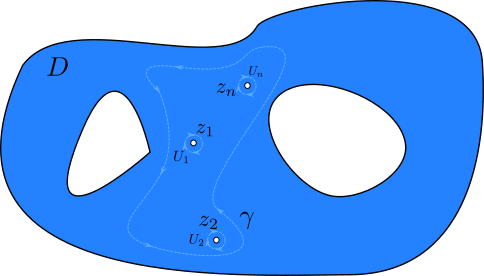
\includegraphics[scale = 1]{path1377.png}
	\end{figure}
$\boxed{=} \displaystyle \sum_{k=1}^n \oint\displaylimits_{U_k} f(z)\,dz \overset{def}{=} \sum_{k=1}^n 2\pi i \residue{z_k}{f(z)} = 2\pi i \sum_{k=1}^n \residue{z_k}{f(z)}$.
\end{proof}

\begin{example}
$\displaystyle \oint\displaylimits_{|z-2|=2} \frac{z\,dz}{(z-1)(z-2)} \boxed{=}$\\
Розглянемо функцію $\displaystyle f(z) = \frac{z}{(z-1)(z-2)}$. Тут $z = 1, z = 2$ - обидві полюси 1 порядку, тому\\
$\displaystyle \residue{1}{f(z)} = \lim_{z \to 1} \frac{z}{(z-1)(z-2)} (z-1) = -1$\\
$\displaystyle \residue{2}{f(z)} = \lim_{z \to 2} \frac{z}{(z-1)(z-2)} (z-2) = 2$\\
$\boxed{=} 2 \pi i (\residue{1}{f(z)} + \residue{2}{f(z)}) = 2 \pi i$.
\end{example}

\begin{theorem}[Теорема Коші для лишків, 2*]
Задано функцію $f$ - аналітична в $\mathbb{C}$ за винятком скінченної кількості особливих точок $z_1,z_2,\cdots z_n$. \\
Тоді (див. п. 2.9.3. про лишки в $\infty$) $\displaystyle\sum_{k=1}^{n} \residue{z_k}{f(z)} + \residue{\infty}{f(z)} = 0$.
\end{theorem}

\begin{proof}
Розглянемо замкнений контур $\gamma$, що охоплює всі скінченні особливі точки\\
$\displaystyle \residue{\infty}{f(z)} \overset{\text{def}}{=} \frac{1}{2 \pi i} \oint\displaylimits_{\gamma^-} f(z) \,dz = -\frac{1}{2 \pi i} \oint\displaylimits_{\gamma^+} f(z) \,dz = -\frac{1}{2 \pi i} \cdot 2 \pi i\sum_{k=1}^{n}  \residue{z_k}{f(z)}$\\
$\Rightarrow\displaystyle \sum_{k=1}^{n} \residue{z_k}{f(z)} + \residue{\infty}{f(z)} = 0$
\end{proof}

\begin{remark}
Ми не розглядаємо нескінченну кількість особливих точок, оскільки в цьому випадку з'являються граничні точки. А вони не є ізольованими.
\end{remark}

\subsection{Нескінченна особлива точка}
Хочеться піти здалеку, як зрозуміти цю дивну точку, $z = \infty$.\\
Вважаємо, що в нас є система координат, на якій ми побудуємо сферу радіусом $1\over{2}$ таким чином, щоб сфера торкалась площини $XOY$ в точці $(0,0)$. На площині $XOY$ кожна точка з координатами $(x,y)$ буде відповідати значенню комплексного числа $z = x + iy$. І позначимо верхню точку сфери $N$.
\begin{figure}[H]
\centerline{\includegraphics[scale = 0.7]{Riemann_sphere.png}}
\end{figure}
Через точку із $XOY$ (скажімо, т. $P$) та т. $N$ проведемо пряму. Отримаємо точку перетину $M$. Тоді кожна точка сфери відповідає точці $XOY$. Звідси якщо взяти якийсь окіл т. $M$, то вона відповідатиме окілу т. $P$.\\
І навпаки: кожна точка $XOY$ відповідає т. сфери... Але не в т. $N$. Взагалі кажучи, жодна точка $XOY$ не відповідає $N$, оскільки пряма буде паралельна до цієї площини. Тому вирішили, що для т. $N$ ставимо в відповідність т. $z = \infty$.\\
Тепер візьмемо окіл т. $N$ радіуса $D$ і подивимось, який окіл відповідає $XOY$. Принаймні це нам знадобиться, якщо ми хочемо розкласти в ряд Лорана.\\
Отримаємо площину вигляду $|z|>D$. Тобто всі точки комплексної площини за межами кола.
\begin{figure}[H]
\centerline{\includegraphics[scale = 0.5]{Riemann_sphereINF.png}}
\end{figure}
Якось так.

\subsubsection{Розклад в Лорана}
Нехай $f$ - аналітична на $\{z: |z| > D\}$. Зробимо перетворення $\displaystyle w = \frac{1}{z}$. Точка $z = \infty$ переводить в точку $w = 0$.\\
Розглянемо ряд Лорана в околі $z = \infty$, тобто для $\{z: |z|>D\}$.\\
$\displaystyle f(z) = f\left(\frac{1}{w}\right) = g(w) \boxed{=} $\\
$|z|>D \iff \displaystyle \abs{\frac{1}{w}} > D \iff |w| < \frac{1}{D}$.\\
$\displaystyle \boxed{=} \sum_{k=1}^{\infty} \frac{c_{-k}}{w^k} + \sum_{n=0}^{\infty} c_n w^n = \underbrace{\sum_{k=1}^{\infty} c_{-k}z^k}_{\textrm{головна частина}} + \underbrace{\sum_{n=0}^{\infty} \frac{c_n}{z_n}}_{\textrm{правильна частина}}$.\\
Отримали ряд Лорана в околі $z = \infty$.
\bigskip \\
Коефіцієнти ряду обчислюються ось так:\\
$\displaystyle c_n = \frac{1}{2 \pi i} \oint\displaylimits_{\gamma} \frac{g(w)}{w^{n+1}} \,dw \boxed{=} $\\
Проведемо заміну: $\displaystyle w = \frac{1}{z} \Rightarrow g(w) = f(z) \implies dw = -\frac{1}{z^2} \,dz$.\\
І візьмемо контур $|w|=\rho$ - коло, щоб було простіше рахувати. Тоді якщо $w = \rho e^{it}, t \in \displaystyle \vec{[0, 2\pi]}$ - обхід проти годинникової стрілки, то\\
$z = \displaystyle \frac{1}{w} = \frac{1}{\rho} e^{-it}, t \in \displaystyle \vec{[2 \pi, 0]}$ - обхід за годинниковою стрілкою.\\
Отже, $|w| = \rho$ переводиться в $\displaystyle |z| = \frac{1}{\rho}$ зі зміном орієнтації.\\
Тому $\gamma \rightarrow \gamma_{-}$ (перед інтегралом буде ще знак мінус).\\
$\displaystyle \boxed{=} - \frac{1}{2 \pi i} \oint\displaylimits_{\gamma} -\frac{f(z) z^{n+1}}{z^2} \,dz = \frac{1}{2 \pi i} \oint\displaylimits_{\gamma} f(z) z^{n-1} \,dz$.\\
Остаточно:
\begin{align*}
f(z) = \underbrace{\sum_{k=1}^{\infty} c_{-k}z^k}_{\textrm{головна частина}} + \underbrace{\sum_{n=0}^{\infty} \frac{c_n}{z_n}}_{\textrm{правильна частина}} \\
c_n = \frac{1}{2 \pi i} \oint\displaylimits_{\gamma} f(z) z^{n-1} \,dz
\end{align*}

\subsubsection{Ізольовані точки}
\begin{definition}
Точка $z=\infty$ називається \textbf{ізольованою особливою для} $f(z)$, якщо $\exists R:$ в області $\{z: |z|>R\}$ функція $f$ - аналітична.
\end{definition}

\textbf{Класифікація ізольованих точок}:\\
	 - \textbf{усувна}, якщо $\displaystyle\exists \lim_{z \to \infty} f(z) \in \mathbb{C}$;\\
	 - \textbf{полюс}, якщо $\displaystyle\exists \lim_{z \to \infty} f(z) = \infty$;\\
	 - \textbf{суттєва}, якщо $\displaystyle \nexists \lim_{z \to \infty} f(z)$.
	 \bigskip \\
Порядок полюса $z = \infty$:
$\displaystyle \exists \lim_{z \to \infty} f(z) = \infty \iff \lim_{z \to \infty} \frac{1}{f(z)} = 0$.\\
Тоді порядком цієї точки функції $f(z)$ називають кратність нуля функції $\displaystyle h(z) = \frac{1}{f(z)}$, а точніше кратність нуля точки $w_0 = 0$ для функції $\displaystyle g(w) = h\left(\frac{1}{w}\right)$.

\begin{proposition} Маємо:\\
Точка $z = \infty$ - усувна $\iff$ ряд Лорана не містить головної частини.\\
Точка $z = \infty$ - полюс порядку $k$ $\iff$ ряд Лорана містить $k$ доданків головної частини.\\
Точка $z = \infty$ - суттєва $\iff$ ряд Лорана містить нескінченну кількість доданків головної частини.\\
\textit{Всі ці твердження випливають з того, що ряд Лорана в $z = \infty$ - це ряд Лорана в $\displaystyle w = \frac{1}{z} = 0$.}
\end{proposition}

\subsubsection{Лишки}
\begin{definition}
Задано функцію $f$ та ізольована точка $z = \infty$.\\
\textbf{Лишком функції} $f(z)$ \textbf{в т.} $\infty$ називається ось такий вираз:
\begin{align*}
\residue{\infty}{f(z)} = \frac{1}{2 \pi i} \oint\displaylimits_{\gamma_-} f(z)\,dz
\end{align*}
За межами $\gamma_-$ немає інших особливих точок.
\end{definition}

\begin{theorem}
Задана функція $f$ та ізольована точка $z = \infty$. Тоді $\residue{\infty}{f(z)} = -c_1$.\\
\textit{Випливає з розкладу ряду Лорана та визначення коефіцієнтів}
\end{theorem}

Шукати лишки можна за аналогічними теоремами в залежності від класифікації ізольованої точки.

\begin{example}
Визначити тип ізольованої точки $z_* = \infty$ для функції $f(z) = 1 - z + 2z^2$ і знайти лишок.\\
Тут вже функція розкладена в ряд Лорана в т. $z_* = \infty$, що містить дві доданки головної частини. А тому $z_* = \infty$ - полюс порядку 2.\\
Коефіцієнт перед $z$: $c_1 = -1$. Тому звідси $\residue{\infty}{f(z)} = -c_1 = 1$.
\end{example}

\subsection{Застосування лишків до дійсних інтегралів}
I. $R(x,y)$ - дробово-раціональна функція від $x,y$\\
Розглянемо $\displaystyle \int_{0}^{2\pi} R(\cos x, \sin x) \,dx \boxed{=}$\\
Заміна: $\displaystyle \cos x = \frac{e^{ix}+e^{-ix}}{2}, \sin x = \frac{e^{ix}-e^{-ix}}{2i}$\\
$\displaystyle e^{ix} = z \Rightarrow z \in \{z: |z| = 1\}$ - коло радіуса 1, що рухається проти годинникової стрілки\\
$\displaystyle e^{-ix} = \frac{1}{z}$\\
$\Rightarrow \displaystyle \cos x = \frac{z+\frac{1}{z}}{2} = \frac{z^2+1}{2z}$\\
$\Rightarrow \displaystyle \sin x = \frac{z-\frac{1}{z}}{2} = \frac{z^2-1}{2zi}$\\
$dz = i e^{ix}\,dx$\\
$\displaystyle \boxed{=} -\oint\displaylimits_{|z|=1} iR\left(\frac{z^2+1}{2z}, \frac{z^2-1}{2zi}\right) \frac{dz}{z} \boxed{=}$\\
Підінтегральна функція - дробово-раціональний вираз від $z$, що має скінченну кількість особливих точок, в тому числі скінченну кількість полюсів в колі $|z|=1$\\
$\displaystyle \boxed{=} 2 \pi \sum_{j=1}^n \residue{z_j}{\left(R\left(\frac{z^2+1}{2z}, \frac{z^2-1}{2zi}\right) \frac{1}{z}\right)}$\\
\hugespace
\textbf{Example.} $\displaystyle \int_{0}^{2\pi} \frac{dx}{2 + \cos x + \sin x} \boxed{=}$\\
Проводимо ту саму заміну:  $\displaystyle z = e^{ix} \Rightarrow \cos x = \frac{z^2+1}{2z}, \sin x = \frac{z^2-1}{2zi}$\\
$\displaystyle dx = \frac{-i}{z} \,dz$\\
$\displaystyle \boxed{=} -i\oint\displaylimits_{|z|=1} \frac{1}{2+ \frac{z^2+1}{2z} + \frac{z^2-1}{2zi}} \frac{dz}{z} = \oint\displaylimits_{|z|=1} \frac{2}{4iz + iz^2 + i + z^2 - 1} \,dz = \\ = \oint\displaylimits_{|z|=1} \frac{2}{z^2(1+i) + 4iz + i-1} \,dz \boxed{=}$\\
Перепозначу: $\displaystyle f(z) = \frac{1}{z^2(1+i)+4iz+i-1}$\\
Подивимось на особливі точки підінтегрального виразу:\\
$z^2(1+i)+4iz+i-1=0$\\
$z_1 = \displaystyle \frac{\sqrt{2}-2}{2} + i \frac{\sqrt{2}-2}{2}$\\
$z_2 = \displaystyle -\frac{\sqrt{2}+2}{2} - i \frac{\sqrt{2}+2}{2}$\\
Обидва вони полюси першої кратності. Лише одна точка - $z_1$ - потрапляє в коло $|z| =1$\\
$\displaystyle f(z) = \frac{1}{(1+i)(z-z_1)(z-z_2)}$\\
$\displaystyle \boxed{=} 2 \cdot 2\pi i \residue{z_1}{f(z)} = 4 \pi i \lim_{z \to z_1} \frac{1}{(1+i)(z-z_2)} = 4 \pi i \frac{1}{(1+i)(z_1 - z_2)} = \dots = \\ = \sqrt{2} \pi$
\hugespace

II. Невласні дійсні інтеграли\\
Розглянемо $\displaystyle \int_{-\infty}^{+\infty} f(x) dx \overset{\textrm{обчислимо}}{=} = p.v. \int_{-\infty}^{+\infty} f(x) dx = \lim_{A \to \infty} \int_{-A}^{+A} f(x) dx$
\hugespace
\textbf{Theorem.} Задана функція $f(x)$ на $\mathbb{R}$ така, що вона продовжується аналітично на верхню півплощину $\mathbb{C}$ (тобто $\Im z \geq 0$) за виключенням скінченної кількості точок $z_1, \cdots, z_n$\\
Наша функція $f(z)$ така, що $\displaystyle \exists \lim_{|z| \to \infty} |z f(z)| = 0$\\
Тоді \begin{align*}
\int_{-\infty}^{+\infty} f(x) dx = 2 \pi i \sum_{j=1}^n \residue{z_j}{f(z)}
\end{align*}
\textbf{Proof.}\\
$\displaystyle \int_{-\infty}^{+\infty} f(x) dx = \displaystyle \lim_{R \to \infty} \int_{-R}^{R} f(x) dx = \\
= \lim_{R \to \infty} \left(\int\displaylimits_{[\overrightarrow{-R,R}]} f(z)dz + \int\displaylimits_{\underset{\Im z \geq 0}{|z|=R}} f(z)dz - \int\displaylimits_{ \underset{\Im z \geq 0}{|z|=R}} f(z)dz \right) = \\ =
\lim_{R \to \infty} \left(\int\displaylimits_{[\overrightarrow{-R,R}] \cup \underset{\Im z \geq 0}{|z|=R}} f(z)dz - \int\displaylimits_{ \underset{\Im z \geq 0}{|z|=R}} f(z)dz \right) \boxed{=}
$\\
Обидва інтеграли мають напрямок в противогодинникової стрілки\\
Розглянемо $\displaystyle \abs{\int\displaylimits_{ \underset{\Im z \geq 0}{|z|=R}} f(z)dz} \leq \int\displaylimits_{ \underset{\Im z \geq 0}{|z|=R}} \abs{f(z)}\abs{dz} = $\\
Заміна: $z = Re^{it}, t \in [0, \pi], |dz| = R\,dt$\\
$\displaystyle = \int_0^\pi f(Re^{it}) R\,dt$\\
Нас цікавить границя цього модулю:\\
$\displaystyle \lim_{R \to \infty} f(Re^{it})R = \lim_{\underset{|z|=R}{|z| \to \infty}} |z f(z)| \overset{\textrm{умова}}{=} 0$\\
Звідси $\displaystyle \lim_{R \to \infty} \int_0^\pi f(Re^{it}) R\,dt = 0$\\
\\
$\displaystyle \boxed{=}  \lim_{R \to \infty} \int\displaylimits_{[\overrightarrow{-R,R}] \cup \underset{\Im z \geq 0}{|z|=R}} f(z)dz = $\\
Для великих $R$ наш контур охоплює всі особливі точки $f(z)$. Але наша кількість скінченна\\
$\displaystyle = \sum_{j=1}^n \residue{z_j}{f(z)}$ $\blacksquare$
\hugespace

\textbf{Example.} $\displaystyle \int_{-\infty}^{+\infty} \frac{x^2+1}{x^4+1}\,dx = \boxed{=}$\\
Розглянемо функцію $\displaystyle f(z) = \frac{z^2+1}{z^4+1}$, при цьому $\Im z > 0$\\
Для неї є чотири проблемні точки $z_1, z_2, z_3, z_4$, але потрапляють лише $z_1, z_4$ - два полюси, обидва першого порядку:\\
$\displaystyle z_1 = \frac{\sqrt{2}}{2} + \frac{\sqrt{2}}{2} i \Rightarrow \residue{z_1}{f(z)} = \frac{i+1}{(z_1-z_2)(z_1-z_3)(z_1-z_4)^2} = \frac{1}{2 \sqrt{2} i}$\\
$\displaystyle z_4 = -\frac{\sqrt{2}}{2} + \frac{\sqrt{2}}{2} i \Rightarrow \residue{z_4}{f(z)} = \frac{-i+1}{(z_4-z_1)(z_4-z_2)(z_4-z_3)^2} = \frac{1}{2 \sqrt{2} i}$\\
І нарешті, треба перевірити умову: $\displaystyle \lim_{z \to \infty} z f(z) = \lim_{z \to \infty} z \cdot \frac{z^2+1}{z^4+1} = 0$\\
$\displaystyle \boxed{=} 2 \pi i \frac{1}{\sqrt{2} i } = \pi \sqrt{2}$
\hugespace

III. Розглянемо $\displaystyle \int_{-\infty}^{+\infty} f(x) \cos \alpha x \,dx $ або $\displaystyle \int_{-\infty}^{+\infty} f(x) \sin \alpha x \,dx $\\
Варто зауважити, що $\cos \alpha x = \Re e^{i \alpha x}$, $\sin \alpha x = \Im e^{i \alpha x}$\\
Тому:\\
$\displaystyle \int_{-\infty}^{+\infty} f(x) \cos \alpha x \,dx = \Re \int_{-\infty}^{+\infty} f(x) e^{i \alpha x} \,dx$\\
$\displaystyle \int_{-\infty}^{+\infty} f(x) \sin \alpha x \,dx = \Im \int_{-\infty}^{+\infty} f(x) e^{i \alpha x} \,dx$\\
Тоді далі будемо розглядати \\ $\displaystyle \int_{-\infty}^{+\infty} f(x) e^{i \alpha x} \,dx = p.v. \int_{-\infty}^{+\infty} f(x) e^{i \alpha x} \,dx = \lim_{R \to \infty} \int_{-R}^{R} f(x) e^{i \alpha x} \,dx$
\hugespace
\textbf{Lemma. Лема Жордана}\\
Задана функція $f$ - аналітична на верхній півплощині $\mathbb{C}$ за виключенням скінченної кількості особливих точок.\\
Відомо, що $\displaystyle \lim_{|z| \to \infty} \max_{\underset{\Im z \geq 0}{|z|=R}} \abs{f(z)} = 0$. Тоді
\begin{align*}
\lim_{R \to \infty} \int\displaylimits_{\underset{\Im z \geq 0}{|z|=R}} f(z)e^{i \alpha z} \,dz = 0
\end{align*}
\textbf{Proof.}\\
$\displaystyle \abs{\int\displaylimits_{\underset{\Im z \geq 0}{|z|=R}} f(z)e^{i \alpha z} \,dz} \leq \int\displaylimits_{\underset{\Im z \geq 0}{|z|=R}} |f(z)e^{i \alpha z}| \,|dz| =$\\
Заміна: $z = Re^{it}, t \in [0, \pi], |dz|=R\,dt$\\
$= \displaystyle \int_0^{pi} \abs{f(Re^{it})e^{iR \alpha e^{it}}} R\,dt \boxed{\leq}$\\
Розглянемо окремо $\displaystyle \abs{e^{iR \alpha e^{it}}} = \abs{e^{iR \alpha (\cos t + i \sin t)}} = \underset{=1}{|e^{iR \alpha \cos t}|} |e^{-\alpha R \sin t}| = e^{-\alpha R \sin t}$\\
$\displaystyle \sin t \geq 
\begin{cases}
 \displaystyle\frac{2}{\pi} t , t \in [0, \frac{\pi}{2}]\\
 \\
 \displaystyle\frac{2}{\pi} (\pi - t), t \in [\frac{\pi}{2}, \pi] \\
\end{cases} \overset{\textrm{позначимо}}{=} g(t)\\
$\\
\begin{figure}[h]
\centerline{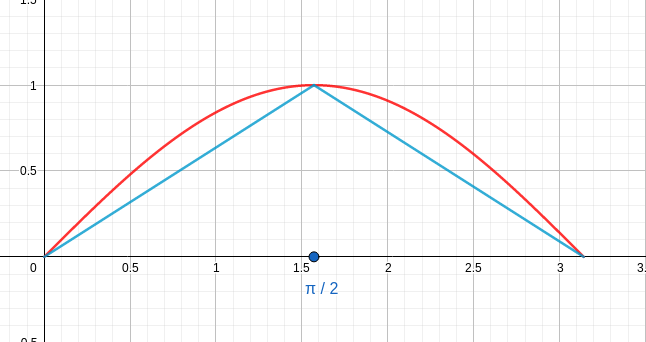
\includegraphics[scale = 0.6]{sinless.png}}
\caption{Червоний - $\sin t$, Синій - $g(t)$}
\end{figure}

Отже,\\
$\displaystyle e^{-\alpha R \sin t} \leq e^{-\alpha R g(t)}$\\
$\displaystyle \boxed{\leq} \max_{\underset{\Im z \geq 0}{|z|=R}} \abs{f(z)} \int_0^\pi e^{-\alpha R g(t)} R\,dt = \max_{\underset{\Im z \geq 0}{|z|=R}} \abs{f(z)} \left(\int_0^{\frac{\pi}{2}} e^{-\alpha R \frac{2\pi}{t}} R\,dt + \int_{\frac{\pi}{2}}^{\pi} e^{-\alpha R \frac{2}{\pi}(\pi-t)} R\,dt \right) = \\ = \max_{\underset{\Im z \geq 0}{|z|=R}} \abs{f(z)} R \left(-\frac{\pi}{2 \alpha R} (e^{-\alpha R}-1) + \frac{\pi}{2\alpha R} (1 - e^{-\alpha R}) \right) = \max_{\underset{\Im z \geq 0}{|z|=R}} \abs{f(z)} \left(-\frac{\pi}{\alpha}e^{-\alpha R} + \frac{\pi}{\alpha} \right) = \\ = \max_{\underset{\Im z \geq 0}{|z|=R}} \abs{f(z)} \frac{\pi}{\alpha} \left(1 - e^{-\alpha R} \right)$\\
Якщо $R \to \infty$, то отриманий вираз прямує до нуля. Таким чином,\\
$\displaystyle \lim_{R \to \infty} \int\displaylimits_{\underset{\Im z \geq 0}{|z|=R}} f(z)e^{i \alpha z} \,dz = 0$ $\blacksquare$
\hugespace
\textbf{Theorem.} Задана функція $f(x)$ на $\mathbb{R}$ така, що вона продовжується аналітично на верхню півплощину $\mathbb{C}$ за виключенням скінченної кількості точок $z_1, \cdots, z_n$\\
Наша функція $f(z)$ така, що $\exists \displaystyle \lim_{|z| \to \infty} \max_{\underset{\Im z \geq 0}{|z|=R}} \abs{f(z)} = 0$\\
Тоді
\begin{align*}
\int_{-\infty}^{+\infty} f(x) e^{i \alpha x} \,dx = 2 \pi i \sum_{j=1}^n \residue{z_j}{f(z)e^{i \alpha z}}
\end{align*}
\textbf{Proof.}\\
$\displaystyle \int_{-\infty}^{+\infty} f(x) e^{i \alpha x} \,dx = \lim_{R \to \infty} \left(\int\displaylimits_{[\overrightarrow{-R,R}]} f(z)e^{i \alpha z}dz + \int\displaylimits_{\underset{\Im z \geq 0}{|z|=R}} f(z)e^{i \alpha z}dz - \int\displaylimits_{ \underset{\Im z \geq 0}{|z|=R}} f(z)e^{i \alpha z}dz \right) = \\ 
= \lim_{R \to \infty} \left(\int\displaylimits_{[\overrightarrow{-R,R}] \cup \underset{\Im z \geq 0}{|z|=R}} f(z)e^{i \alpha z}dz - \int\displaylimits_{ \underset{\Im z \geq 0}{|z|=R}} f(z)e^{i \alpha z}dz \right) \overset{\textrm{Lm. Жордана}}{=} \\ = \lim_{R \to \infty} (2 \pi i)\sum_{j=1}^n \residue{z_j}{f(z)e^{i \alpha z}} = 2 \pi i \sum_{j=1}^n \residue{z_j}{f(z)e^{i \alpha z}}$ $\blacksquare$
\hugespace

\textbf{Example.} $\displaystyle \int_{-\infty}^{+\infty} \frac{x \sin x}{x^2+4x+20} = \Im \int_{-\infty}^{+\infty} \frac{x e^{ix}}{x^2+4x+20} \boxed{=}$\\
Розглянемо функцію $\displaystyle f(z) = \frac{z}{z^2+4z+20}$, де $\Im z \geq 0$ \\
$z_1, z_2$ - корені знаменнику, але $z_1 = -2 + 4i$ - полюс першого порядку - потрапляє в нашу область\\
Більш того, $\displaystyle \lim_{z \to \infty} f(z) = \lim_{z \to \infty} \frac{z}{z^2+4z+20} = 0$\\
$\displaystyle \boxed{=} \Im[ 2\pi i \residue{z_1}{f(z)e^{iz}}] = \Im\left[ 2\pi i \lim_{z \to -2+4i} \frac{ze^{iz}}{2+2+4i}\right] = \dots = \\ = \Im\left[ \frac{\pi}{4} e^{-4} (4i-2)(\cos 2 - i \sin 2) \right] = \frac{\pi}{4}e^{-4} (4\cos 2 + 2 \sin 2)$
\newpage


%END OF PARAGRAPH 2%


\section{Ряди Фур'є}
\subsection*{Передмова до цієї теми}
Зазвичай аби розповісти про ряди Фур'є та їхнє появлення на світ, необіхдно знати багато тем з лінійної алгебри 2 семестру. Користуючись нагодою, я хочу передати величезний "привіт"  одному викладачу, що максимально завалив зміст дисципліни лін. ал. (із КН ММСА)\\
\\
І водночас двічі вдячний ГБ за уникнення таких складнощів та дав, в принципі, достойне оповідання рядів Фур'є без лінійки.\\
 
\subsection{Початок}
Нехай задана $g(z)$ - аналітична в кільці $K = \{z: 1-\varepsilon_1 <|z|<1+\varepsilon_2 \}$. Причому $\{z: |z|=1\} \subset K$\\
Розкладемо $g(z)$ в ряд Лорана за степенем $z$ в цьому кільці:\\
$\displaystyle g(z) = \sum_{n=-\infty}^{\infty} c_n z^n$,\\
де $\displaystyle c_n = \frac{1}{2 \pi i} \oint\displaylimits_{|z|=1} \frac{g(z)}{z^{n+1}}\,dz$\\
А тепер зробимо наступне:\\
$|z|=1 \Rightarrow z = e^{ix}, x \in [0, 2 \pi]$. Тоді\\
$\displaystyle g(z) = g(e^{ix}) \overset{\textrm{позн}}{=} f(x)$\\
$\displaystyle c_n = \frac{1}{2 \pi i} \oint\displaylimits_{|z|=1} \frac{g(z)}{z^{n+1}}\,dz \overset{z=e^{ix}}{=}  \frac{1}{2 \pi i} \int_0^{2 \pi} \frac{f(x)}{e^{(n+1)ix}} ie^{ix}\,dx = \frac{1}{2 \pi} \int_0^{2 \pi} f(x)e^{-inx}\,dx$\\
Отримали комплексну форму ряду Фур'є\\
$\displaystyle f(x) = \sum_{n=-\infty}^{\infty} c_n e^{inx}, c_n = \frac{1}{2 \pi} \int_0^{2 \pi} f(x)e^{-inx}\,dx$
\hugespace
Є деякі необхідні умови:\\
$f \in D([0, 2\pi]) \iff f$ - $2 \pi$-періодична інтегрована на будь-якому відрізку $\iff$ $f \in D([-\pi, \pi])$\\
За функцією $f(x)$ будуємо ряд Фур'є:\\
$\displaystyle S(x) = \sum_{n=-\infty}^{\infty} c_n e^{inx}, c_n = \frac{1}{2 \pi} \int_0^{2 \pi} f(x)e^{-inx}\,dx$\\
\hugespace
\textbf{Головні питання до цього ряду:}\\
1) збіжність ряду Фур'є\\
2) якщо збігається, то який зв'язок між $S(x)$ та $f(x)$\\
Будемо вивчати для випадку $f(x)$ - дійснозначна функція (в подальшому)\\
\hugespace
Розглянемо ряд Фур'є\\
$\displaystyle \sum_{n=-\infty}^{-1} c_n + c_0 + \displaystyle \sum_{n=1}^{\infty} c_n
= c_0 + \displaystyle \sum_{k=1}^{\infty} c_{-k}e^{-ikx} + \sum_{n=1}^{\infty} c_ne^{inx} \boxed{=}
$\\
Коефіцієнти головної частини: \\ $\displaystyle c_{-k} = \frac{1}{2 \pi} \int_0^{2\pi} f(x)e^{ikx} \,dx = \overline{\frac{1}{2 \pi} \int_0^{2\pi} f(x)e^{-ikx} \,dx} = \overline{c_k}$\\
Тому $c_{-k}e^{-ikx} = \overline{c_k} \overline{e^{ikx}} = \overline{c_k e^{ikx}}$\\
$\displaystyle \boxed{=} c_0 + \sum_{n=1}^{\infty} \left( \underset{\in \mathbb{R}}{\overline{c_n e^{inx}} + c_n e^{inx}} \right) \boxed{=}$\\
Маленький комплексний факт:\\
$\begin{cases}
w = a + ib\\
\overline{w} = a - ib
\end{cases} \Rightarrow w + \overline{w} = 2a = 2\Re w
$\\
$\displaystyle \boxed{=} c_0 + \sum_{n=1}^{\infty} 2 \Re(c_n e^{inx}) \boxed{\boxed{=}}$\\
З'ясуємо більш детально про коефіцієнт:\\
$\displaystyle c_n = \frac{1}{2\pi}\int_0^{2\pi} f(x)e^{-inx}\,dx = \frac{1}{2 \pi} \int_0^{2\pi} f(x) \cos nx \,dx - i \frac{1}{2 \pi} \int_0^{2\pi} f(x) \sin nx \,dx$\\
Тоді:\\
$\displaystyle \Re (c_n e^{inx}) = \\ = \Re\left(\left(\frac{1}{2 \pi} \int_0^{2\pi} f(x) \cos nx \,dx - i \frac{1}{2 \pi} \int_0^{2\pi} f(x) \sin nx \,dx \right) \cdot \left(\cos nx + i \sin nx \right)\right) = \frac{1}{2 \pi i} \left(\int_0^{2 \pi} f(x) \cos nx \,dx \cdot \cos nx + \int_0^{2 \pi} f(x) \sin nx \,dx \cdot \sin nx \right)$\\
$\displaystyle \boxed{\boxed{=}} c_0 + \sum_{n=1}^{\infty} \frac{1}{\pi} \left(\int_0^{2 \pi} f(x) \cos nx \,dx \cdot \cos nx + \int_0^{2 \pi} f(x) \sin nx \,dx \cdot \sin nx \right)$\\
$\displaystyle c_0 = \frac{1}{2 \pi} \int_{0}^{2 \pi} f(x)\,dx$\\
Отримали дійсну формулу ряда Фур'є:
\begin{align*}
f(x) \leadsto \frac{a_0}{2} + \sum_{n=0}^{\infty} a_n \cos nx + b_n \sin nx \\
a_n = \frac{1}{\pi}\int_0^{2\pi} f(x) \cos nx \,dx, n \in \mathbb{N} \setminus \{0\} \\
b_n = \frac{1}{\pi}\int_0^{2\pi} f(x) \sin nx \,dx, n \in \mathbb{N}
\end{align*}
Але ці формули для функції $2\pi$-періодичних
\hugespace
Розглянемо відображення $[0, 2\pi] \leftarrow [0, 2l]$\\
$[0, 2\pi] \rightarrow x$, $\displaystyle x = \frac{t}{l}\pi, t \in [0,2l]$\\
Тоді $\displaystyle f(x) = f(\frac{t}{l}\pi) \overset{\textrm{позн}}{=} g(t)$ - задана на $[0, 2l]$, тобто $2l$-періодична\\
$\displaystyle a_n = \frac{1}{\pi}\int_0^{2\pi} f(x) \cos nx \,dx \overset{\displaystyle x = \frac{t}{l} \pi}{=} \frac{1}{l} \int_0^{2l} g(t) \cos \left( \frac{\pi n t}{l} \right) \,dt$\\
$\displaystyle b_n = \frac{1}{\pi}\int_0^{2\pi} f(x) \sin nx \,dx \overset{\displaystyle x = \frac{t}{l} \pi}{=} \frac{1}{l} \int_0^{2l} g(t) \sin \left( \frac{\pi n t}{l} \right) \,dt$\\
Тоді розклад в ряд:\\
$\displaystyle g(t) \leadsto \displaystyle \frac{a_0}{2} + \sum_{n=0}^{\infty} a_n \cos \left( \frac{\pi n t}{l} \right) + b_n \sin \left( \frac{\pi n t}{l} \right)$\\
Найчастіше зручно шукати коефіцієнти в такому вигляді:\\
$\displaystyle a_n = \frac{1}{l} \int_{-l}^{l} g(t) \cos \left( \frac{\pi n t}{l} \right) \,dt$\\
$\displaystyle b_n = \frac{1}{l} \int_{-l}^{l} g(t) \sin \left( \frac{\pi n t}{l} \right) \,dt$
\hugespace

\subsection{Аналіз збіжності ряду}
\textbf{Lemma 3.2.1. Лема Рімана}\\ Задана функція $f \in D([a,b])$ (навіть в невласному сенсі абсолютно). Тоді
\begin{align*}
1) \int_a^b f(x) \cos \lambda x \,dx \to 0, \lambda \to \infty \\
2) \int_a^b f(x) \sin \lambda x \,dx \to 0, \lambda \to \infty
\end{align*}
\textbf{Proof.}\\
Доведемо перший пукнт, другий аналогічно\\
Ми розглянемо чотири випадки функції $f$:\\
a) $f(x) = c$ (константа)\\
 $\Rightarrow \displaystyle \int_a^b f(x) \cos \lambda x \,dx = \frac{c}{\lambda} \sin \lambda x \Big|_{a}^b = \frac{c}{\lambda} \left(\sin \lambda b - \sin \lambda a \right) \overset{\lambda \to \infty}{\to} 0$
\hugespace
б) $\displaystyle f(x) = \sum_{k=1}^n c_k 1_{<\alpha_k, \beta_k>} (x)$ (проста функція)\\
$\Rightarrow \displaystyle \int_a^b f(x) \cos \lambda x \,dx = \sum_{k=1}^n \int_a^b 1_{<\alpha_k, \beta_k>} (x) c_k \cos \lambda x \,dx = \sum_{k=1}^n c_k \int_{\alpha_k}^{\beta_k} \cos \lambda x \,dx = \frac{1}{\lambda} \sum_{k=1}^n c_k (\sin \lambda \beta_k - \sin \lambda \alpha_k) \overset{\lambda \to \infty}{\to} 0$\\
\hugespace
в) $f \in D([a,b])$, або $\exists \{p_n(x), n \geq 1\}: p_n \rightrightarrows f$ (інтегрована функція)\\
$\Rightarrow \displaystyle \forall \varepsilon: \exists N: \sup_{x \in [a,b]} |p_N(x) - f(x)| < \varepsilon \iff \\ \forall x \in [a,b]: p_N(x) - \varepsilon <f(x) < p_N(x) + \varepsilon$\\
$\Rightarrow \displaystyle \abs{\int_a^b f(x) \cos \lambda x \,dx - \int_a^b p_N(x) \cos \lambda x \,dx} = \abs{\int_a^b (f(x) - p_N(x)) \cos \lambda x \,dx} \leq \\ \leq \int_a^b |f(x)-p_N(x)| |\cos \lambda x| \,dx \leq \int_a^b \varepsilon \,dx = \varepsilon(b-a)$\\
Таким чином оскільки за п. б), $\displaystyle \int_a^b p_N(x) \cos \lambda x \,dx \overset{\lambda \to \infty}{\to} 0$, то\\
$\displaystyle \forall \varepsilon>0: \exists \Lambda: \forall |\lambda| > \Lambda: \abs{\int_a^b p_N(x) \cos \lambda x \,dx} < \varepsilon(b-a)$\\
Звідси маємо:\\
$\displaystyle \abs{\int_a^b f(x) \cos \lambda x \,dx} \leq \abs{\int_a^b f(x) \cos \lambda x \,dx-\int_a^b p_N(x) \cos \lambda x \,dx} + \abs{\int_a^b p_N(x) \cos \lambda x \,dx} \\ < 2\varepsilon(b-a)$\\
Отже, за означенням, $\displaystyle \int_a^b f(x) \cos \lambda x \,dx \overset{\lambda \to \infty}{\to} 0$\\
\hugespace
г) випадок невласного інтегралу, що збіжний абсолютно, тобто (наприклад) \\ $\displaystyle \int_a^b f(x) \cos \lambda x \,dx = \lim_{\delta \to 0+} \int_a^{b-\delta} f(x) \cos \lambda x \,dx$
\\
(аналогічно для особливої точки $a$, або коли маємо безліч особливих точок $c_1,\dots,c_n \in (a,b))$\\
$\displaystyle \abs{\int_a^b f(x) \cos \lambda x \,dx} = \abs{\int_a^{b-\delta} f(x) \cos \lambda x \,dx + \int_{b-\delta}^b f(x) \cos \lambda x \,dx} \leq \\ \leq \abs{\int_a^{b-\delta} f(x) \cos \lambda x \,dx} + \int_{b-\delta}^b |f(x)| |\cos \lambda x| \,dx \leq \\ \leq \abs{\int_a^{b-\delta} f(x) \cos \lambda x \,dx} + \int_{b-\delta}^b |f(x)| | \,dx \boxed{<}$\\
Оскільки $\displaystyle \int_a^b |f(x)|\,dx$ збігається, то $\displaystyle \forall \varepsilon>0: \exists \delta: \int_{b-\delta}^b |f(x)|\,dx < \frac{\varepsilon}{2}$\\
Більш того, за п. в), $\displaystyle \int_a^{b-\delta} f(x) \cos \lambda x \,dx \overset{\lambda \to \infty}{\to} 0$, тому $\displaystyle \exists \Lambda: \forall |\lambda|>\Lambda: \abs{\int_a^{b-\delta} f(x) \cos \lambda x \,dx} < \frac{\varepsilon}{2}$\\
$\displaystyle \boxed{<} \frac{\varepsilon}{2} + \frac{\varepsilon}{2} = \varepsilon$\\
Отже, за означенням, $\displaystyle \int_a^b f(x) \cos \lambda x \,dx \overset{\lambda \to \infty}{\to} 0$ $\blacksquare$
\hugespace

Розглянемо частковий ряд:
$\displaystyle S_k(x) = \frac{a_0}{2} + \sum_{n=1}^k a_n \cos nx + b_n \sin nx$, де\\
$\displaystyle a_n = \frac{1}{\pi} \int_{-\pi}^{\pi} f(t) \cos nt \,dt$, 
$\displaystyle b_n = \frac{1}{\pi} \int_{-\pi}^{\pi} f(t) \sin nt \,dt$\\
Тоді,\\$\displaystyle S_k(x) = \frac{1}{2\pi} \int_{-\pi}^{\pi} f(t)\,dt + \frac{1}{\pi} \sum_{n=1}^k \int_{-\pi}^{\pi} f(t) \cos nt \,dt \cos nx + \int_{-\pi}^{\pi} f(t) \sin nt \,dt \sin nx = \\
=\frac{1}{2\pi} \int_{-\pi}^{\pi} f(t)\,dt + \frac{1}{\pi} \sum_{n=1}^k \int_{-\pi}^{\pi} f(t) (\cos nt \cos nx + \sin nt \sin nx) \,dt = \\
= \frac{1}{2\pi} \int_{-\pi}^{\pi} f(t)\,dt + \frac{1}{\pi} \int_{-\pi}^{\pi} f(t)\sum_{n=1}^k  \cos n(t-x) \,dt = \\
= \frac{1}{\pi} \int_{-\pi}^{\pi} f(t) \left(\frac{1}{2} + \sum_{n=1}^k  \cos n(t-x)  \right)\,dt \boxed{=}
 $\\
 Знайдемо суму підінтегрального виразу:\\
 $\displaystyle \frac{1}{2} + \sum_{n=1}^k  \cos n\alpha = \frac{1}{2} + \sum_{n=1}^k  \frac{\cos n\alpha \sin \frac{\alpha}{2}}{\sin \frac{\alpha}{2}} = \\
 = \frac{1}{2} + \frac{1}{\sin \frac{\alpha}{2}} \cdot \frac{1}{2} \sum_{n=1}^k \left( \sin (\frac{\alpha}{2}+n\alpha) + \sin (\frac{\alpha}{2} - n\alpha) \right) = \\
 = \frac{1}{2} + \frac{1}{2 \sin \frac{\alpha}{2}} \left(\sin \frac{3\alpha}{2} - \sin \frac{\alpha}{2} + \sin \frac{5\alpha}{2} - \sin \frac{3\alpha}{2} + \dots + \sin \frac{(2k+1)\alpha}{2} - \sin \frac{(2k-1)\alpha}{2} \right) \\ 
 = \frac{1}{2} + \frac{1}{2 \sin \frac{\alpha}{2}} \left(\sin \frac{(2k+1)\alpha}{2} - \sin \frac{\alpha}{2} \right) = \frac{\sin (\frac{(2k+1)\alpha}{2})}{2 \sin (\frac{\alpha}{2})}
 $\\
 \vspace{5mm}\\
 $\displaystyle \boxed{=} \frac{1}{\pi} \int_{-\pi}^{\pi} f(t) \frac{\sin (\frac{(2k+1)(t-x)}{2})}{2 \sin (\frac{(t-x)}{2})} \,dt \overset{t-x=u}{=}
 \frac{1}{2\pi} \int_{-\pi-x}^{\pi-x} f(u+x) \frac{\sin (\frac{(2k+1)}{2}u)}{\sin (\frac{1}{2}u)} \,du =
 $\\
Наша функція $f$ - $2 \pi$-періодична, також і друга функція (як сума $\cos$). Тоді границю $[-\pi-x, \pi-x]$ можна замінити на $[-\pi, \pi]$\\
 $\displaystyle = \frac{1}{2\pi} \int_{-\pi}^{\pi} f(u+x) \frac{\sin (\frac{(2k+1)}{2}u)}{ \sin (\frac{1}{2}u)} \,du = \\
 = \frac{1}{2\pi} \int_{0}^{\pi} f(u+x) \frac{\sin (\frac{(2k+1)}{2}u)}{ \sin (\frac{1}{2}u)} \,du + \frac{1}{2\pi} \int_{-\pi}^{0} f(u+x) \frac{\sin (\frac{(2k+1)}{2}u)}{ \sin (\frac{1}{2}u)} \,du \boxed{=}
 $\\
Зробимо заміну в другому інтегралі: $u = -v$ і замінимо потім на літеру $u$. Отримаємо наступне\\
$\displaystyle \boxed{=} \frac{1}{2\pi} \int_{0}^{\pi} f(x+u) \frac{\sin (\frac{(2k+1)}{2}u)}{ \sin (\frac{1}{2}u)} + f(x-u) \frac{\sin (\frac{(2k+1)}{2}u)}{ \sin (\frac{1}{2}u)} \,du = \\
= \frac{1}{\pi} \int_{0}^{\pi} (f(x+u)+f(x-u)) \frac{\sin (\frac{(2k+1)}{2}u)}{2 \sin (\frac{1}{2}u)} \,du$\\
Таким чином ми довели теорему:
\hugespace
\textbf{Theorem 3.2.2.} Задана функція $f$ - $2 \pi$-періодична, інтегрована. Тоді $\displaystyle S_k(x) = \frac{a_0}{2} + \sum_{n=1}^k a_n \cos nx + b_n \sin nx$ - часткова сума ряду Фур'є - дорівнює іншому виразу:
\begin{align*}
S_k(x) = \frac{1}{\pi} \int_{0}^{\pi} (f(x+u)+f(x-u)) D_k(u) \,du
\end{align*}
\hugespace
\textbf{Перепозначення}: $\displaystyle \frac{\sin (\frac{(2k+1)}{2}u)}{2 \sin (\frac{1}{2}u)} = \frac{1}{2} + \sum_{n=1}^k \cos ku = D_k(u)$ - ядро Діріхле
\hugespace
\textbf{Властивості ядра Діріхле:}\\
1) $D_k(u)$ - парна, $2 \pi$-періодична функція\\
2) $\displaystyle \frac{1}{\pi} \int_{-\pi}^{\pi} D_k(u) \,du = 1$\\
\textbf{Proof.}\\
1. \textit{Вже доводили під час муток з формулами}\\
2. $\displaystyle \int_{-\pi}^{\pi} D_k(u) \,du = \int_{-\pi}^{\pi} \frac{1}{2} \,du + \sum_{n=1}^k \int_{-\pi}^{\pi} \cos ku \,du = \frac{1}{2} 2 \pi = \pi$ $\blacksquare$
\hugespace
Але нас ще цікавить збіжність часткового ряду\\
Розглянемо рівність:\\
$\displaystyle S_k(x) - c = \frac{1}{\pi} \int_{0}^{\pi} (f(x+u)+f(x-u)) D_k(u) \,du - c \frac{1}{\pi} \int_{-\pi}^{\pi} D_k(u) \,du = \\
= \frac{1}{\pi} \int_{0}^{\pi} (f(x+u)+f(x-u)) D_k(u) \,du - c \frac{2}{\pi} \int_{0}^{\pi} D_k(u) \,du = \\
= \frac{1}{\pi} \int_{0}^{\pi} (f(x+u)+f(x-u)-2c) D_k(u) \,du =
$\\
Позначимо $f(x+u)+f(x-u)-2c= g_{c,x}(u)$\\
$\displaystyle = \frac{1}{\pi} \int_{0}^{\pi} g_{c,x}(u) D_k(u) \,du$\\
Сформулюємо зараз нову теорему та доведемо її:
\hugespace
\textbf{Theorem 3.2.3. Ознака Діні (для рядів Фур'є)}\\
Задана функція $f$ - $2\pi$-періодчина, інтегрована.\\ Якщо $\exists \delta > 0: \displaystyle \int_{0}^{\delta} \frac{|g_{c,x}(u)|}{u}\,du$ - збіжний, то $S_k(x) \to c, k \to \infty$\\
\textbf{Proof.}\\
Вже з'ясували, що $\displaystyle S_k(x) - c = \frac{1}{\pi} \int_{0}^{\pi} g_{c,x}(u) D_k(u) \,du = \\
= \frac{1}{\pi} \int_{0}^{\delta} g_{c,x}(u) D_k(u) \,du + \frac{1}{\pi} \int_{\delta}^{\pi} g_{c,x}(u) D_k(u) \,du$\\
Розглянемо доданки по черзі:\\
2. $\displaystyle \frac{1}{\pi}\int_{\delta}^{\pi} g_{c,x}(u) \frac{\sin (\frac{(2k+1)}{2}u)}{2 \sin (\frac{1}{2}u)} \,du \to 0, k \to \infty$\\
за лемою Рімана, тому що $\displaystyle \frac{g_{c,x}(u)}{\sin (\frac{1}{2}u)}$ - функція без особових точок та інтегрована\\
1. $\displaystyle \frac{1}{\pi} \int_{0}^{\delta} g_{c,x}(u) \frac{\sin (\frac{(2k+1)}{2}u)}{2 \sin (\frac{1}{2}u)} \,du$\\
Можемо застосувати лему Рімана. Але треба зазначити, що $\displaystyle \int_{0}^{\delta} \abs{\frac{g_{c,x}(u)}{2 \sin (\frac{u}{2})}} \,du$ збіжний абсолютно. Перевіримо за ознакою порівняння в граничній формі.\\
За умовою теореми, $\displaystyle \int_{0}^{\delta} \frac{|g_{c,x}(u)|}{u}\,du$ - збіжний\\
$\displaystyle \lim_{u \to 0} \frac{\frac{|g_{c,x}(u)|}{2 \sin \frac{u}{2}}}{\frac{|g_{c,x}(u)|}{u}} = \lim_{u \to 0} \frac{u}{2 \sin \frac{u}{2}} = 1$\\
Отже, наш інтеграл збіжний. Тоді за лемою Рімана,\\
$\displaystyle \frac{1}{\pi} \int_{0}^{\delta} g_{c,x}(u) \frac{\sin (\frac{(2k+1)}{2}u)}{2 \sin (\frac{1}{2}u)} \,du \to 0$, $k \to \infty$\\
Остаточно: $S_k(x) - c \to 0$, $k \to \infty$ $\blacksquare$
\hugespace

\textbf{Corollary 3.2.3.(1).} Якщо $f$ - диференційована в т. $x_0$, то \\ $S_k(x_0) \to f(x_0), k \to \infty$\\
\textbf{Proof.}\\
З ознаки Діні випливає, що достатньо перевірити збіжність інтеграла за умовою теореми\\
А зараз:\\
$g_{c,x_0}(u) = f(x_0+u)+f(x_0-u) - 2c \overset{c = f(x_0)}{=} (f(x_0+u)-f(x_0))+(f(x_0-u)-f(x_0))$\\
$\displaystyle \Rightarrow \frac{\abs{g_{c,x_0}(u)}}{u} = \frac{\abs{(f(x_0+u)-f(x_0))+(f(x_0-u)-f(x_0))}}{u} = \\ = \abs{ \frac{f(x_0+u)-f(x_0)}{u} + \frac{f(x_0)-f(x_0-u)}{-u} } \overset{u \to 0}{\to} |f'(x_0)+f'(x_0)| = |f'(x_0)|$\\
Таким чином, у підінтегрованої функції т. $u=0$ є усувною. Тому збіжний\\
Отже, $S_k(x_0) \to f(x_0), k \to \infty$ $\blacksquare$
\hugespace
\textbf{Corollary 3.2.3.(2).} Якщо для $f$ т. $x_0$ є стрибком та містить ліву і праву похідну, то $\displaystyle S_k(x_0) \to \frac{1}{2} (f(x_0,+)+f(x_0,-))$\\
\textbf{Proof.}\\
$\displaystyle c = \frac{1}{2} (f(x_0,+)+f(x_0,-))$\\
Тоді $g_{c,x_0}(u) = f(x_0+u) - f(x_0,+) + f(x_0-u) - f(x_0,-)$\\
$\displaystyle \Rightarrow \frac{\abs{g_{c,x_0}(u)}}{u} = \frac{\abs{(f(x_0+u)-f(x_0,+))+(f(x_0-u)-f(x_0,-))}}{u} = \\ = \abs{ \frac{f(x_0+u)-f(x_0,+)}{u} + \frac{f(x_0,-)-f(x_0-u)}{-u} } \overset{u \to 0}{\to} |f'(x_0,+)+f'(x_0,-)|$\\
Тоді інтеграл в ознаку Діні збігається. Отже $S_k(x_0) \to c$ $\blacksquare$
\hugespace
\textbf{Corollary 3.2.3.(3).} Якщо $f$ задовільняє умові Ліпшиця в околі т. $x_0$, то $S_k(x) \to f(x_0)$, $k \to \infty$\\
\textbf{Proof.}\\
$c = f(x_0)$\\
$\displaystyle \Rightarrow \frac{\abs{g_{c,x_0}(u)}}{u} = \frac{\abs{(f(x_0+u)-f(x_0))+(f(x_0-u)-f(x_0))}}{u} \leq \\ \leq \frac{\abs{f(x_0+u)-f(x_0)}}{u} + \frac{\abs{f(x_0-u)-f(x_0)}}{u} \leq \frac{Lu}{u} + \frac{Lu}{u} = 2L$\\
Тобто така функція є обмеженою в околі $(0, \delta)$, тому є інтегрованою\\
За ознаки Діні, $S_k(x) \to f(x_0)$ $\blacksquare$
\hugespace

Проаналізуємо тепер ряд Фур'є на рівномірну збіжність\\
\textbf{Theorem 3.2.4.} Задана функція $f$ - $2\pi$-періодчина, кусково \\ неперервно-диференційована. Тоді ряд Фур'є рівномірно збігається до $f$\\
\textit{Без доведення, бо я заплутався вже (в цей день ГБ не щастило)}
\hugespace
\textbf{Example.} Розкласти функцію в ряд Фур'є $f(x) = 6-x$ на проміжку $(3, 9)$\\
Її період $T = 6 = 2l$, тому $l=3$\\
Ряд Фур'є містить таку форму:\\
$\displaystyle S(x) = a_0 + \sum_{n=1}^{\infty} a_n \cos \left(\frac{\pi n x}{3} \right) + b_n \sin \left(\frac{\pi n x}{3} \right)$\\
Знайдемо всі коефіцієнти за формулами:\\
$\displaystyle a_n = \frac{1}{3} \int_{3}^{9} (6-x) \cos \left(\frac{\pi n x}{3} \right) \,dx = 0$, $\forall n \neq 0$\\
\textit{Можна міркувати двома способами чому 0: або через періодичність ми можемо змінити границі інтегрування на $[-3,3]$ та використати той факт, що функція - непарна; або площа фігури $[3,6]$ рівний протилежно площі фігури $[6.9]$. Другий варіант все ж таки більш сприятливий}\\
$\displaystyle a_n = \frac{1}{3} \int_{3}^{9} (6-x) \,dx \overset{\textrm{ті самі міркування}}{=} 0$\\
$\displaystyle b_n = \frac{1}{3} \int_{3}^{9} (6-x) \sin \left(\frac{\pi n x}{3} \right) \,dx \overset{u = 6-x}{=} \dots \overset{dv = \sin \left(\frac{\pi n x}{3} \right) \,dx}{=} (-1)^n \frac{6}{\pi n}$\\
Отже, $\displaystyle f(x) \leadsto S(x) = \sum_{n=1}^{\infty} (-1)^n\frac{6}{\pi n} \sin \left(\frac{\pi n x}{3} \right)$\\
У нас тут функція $f$ - диференційована в т. $x \neq 3 + 6k, k \in \mathbb{Z}$. Тоді за першим наслідком ознаки Діні, $S(x) = f(x)$\\
При $x_k = 3 + 6k$ ці точки є стрибками, а також містять ліву та праву похідні. Тоді за другим наслідком ознаки Діні, \\ $S(x_k) = \displaystyle \frac{1}{2} (f(x_k+) + f(x_k-)) = 0$
	\begin{figure}[h]
	\captionsetup{justification=centering}
	\centerline{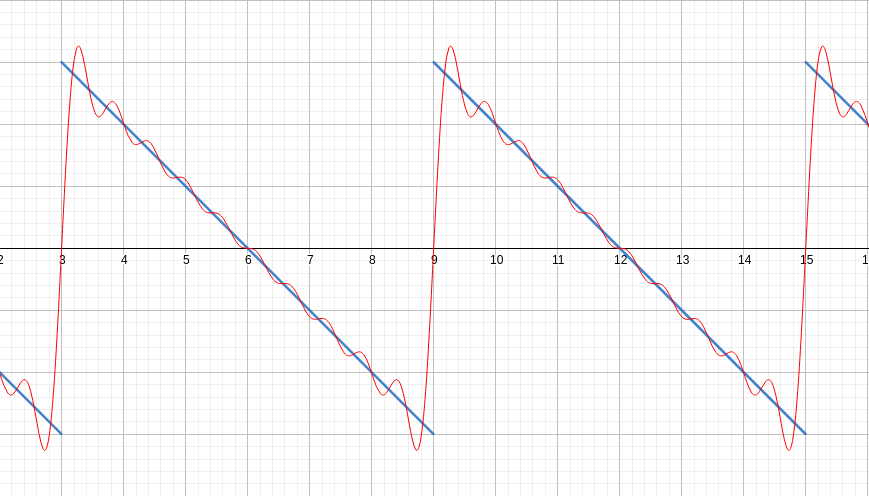
\includegraphics[scale = 0.6]{FourierExpansion.png}}	
	\caption{Червоний графік відповідає розкладу в ряд Фур'є \\ (тут я взяв лише 10 доданків; при нескінченної кількості вона буде схожа за наш початковий графік, оскім стрибків)}
	\end{figure}
\hugespace

\subsection{Додатковий зміст із практики (*)}
\textbf{Властивості ряду Фур'є}\\
1. Якщо на $(-l,l)$ задана непарная функція $f$, то $\forall n \geq 1: a_n = 0$\\
2. Якщо на $(-l,l$ задана парна функція $f$, то $\forall n \geq 1: b_n = 0$\\
3. Якщо $f \in C((-l,l))$, що є $2l$-періодична, то $f \in C(\mathbb{R})$\\
\textit{Залишу без доведення}
\hugespace
\textbf{Розклад функції $f(x)$, що задана на $[0,l)$, в ряд за косінус та сінус}\\
1. $\cos$-Фур'є\\
Продовжимо нашу функцію на $(-l,0)$ парним чином, тобто:\\
$\tilde{f}(x) = \begin{cases} f(x), x \in [0,l) \\ f(-x), x \in (-l,0) \end{cases}$\\
Якщо обережно перевірити, то $\tilde{f}(-x)=\tilde{f}(x)$, $x \in (-l,l)$\\
Оскільки вона парна, то $\forall n \geq 1: b_n = 0$\\
$\Rightarrow \tilde{f}(x) \leadsto S(x) = \displaystyle \frac{a_0}{2} + \sum_{n=1}^{\infty} a_n \cos \left( \frac{\pi n x}{l} \right)$\\
Причому $a_n = \displaystyle \frac{1}{\pi} \int_{-l}^{l} \tilde{f}(x) \cos \left( \frac{\pi n x}{l} \right) \,dx = \frac{2}{l} \int_0^l f(x) \cos \left( \frac{\pi n x}{l} \right)\,dx$\\
Ну а якщо виконаються ознаки Діні, то при $x \in [0,l): \\ S(x) = \tilde{f(x)} = f(x)$
\hugespace
2. $\sin$-Фур'є\\
Продовжимо нашу функцію на $(-l,0)$ непарним чином, тобто:\\
$\tilde{f}(x) = \begin{cases} f(x), x \in [0,l) \\ -f(-x), x \in (-l,0) \end{cases}$\\
Якщо обережно перевірити, то $\tilde{f}(-x)=-\tilde{f}(x)$, $x \in (-l,l)$\\
Оскільки вона непарна, то $\forall n \geq 1: a_n = 0$\\
$\Rightarrow \tilde{f}(x) \leadsto S(x) = \displaystyle \sum_{n=1}^{\infty} b_n \sin \left( \frac{\pi n x}{l} \right)$\\
Причому $b_n = \displaystyle \frac{1}{\pi} \int_{-l}^{l} \tilde{f}(x) \sin \left( \frac{\pi n x}{l} \right) \,dx = \frac{2}{l} \int_0^l f(x) \sin \left( \frac{\pi n x}{l} \right)\,dx$\\
Ну а якщо виконаються ознаки Діні, то при $x \in [0,l): \\ S(x) = \tilde{f(x)} = f(x)$
\hugespace
\textbf{Example. } Розкласти функцію $f(x) = x-1$ в косінус-ряд, $x \in (0,2)$\\
Робимо той самий алгоритм:\\
$\tilde{f}(x) = \begin{cases} x-1, x \in (0,2) \\ -x-1, x \in (-2,0) \end{cases}$ - $4$-періодична, до речі $\Rightarrow l =2$ \\
Обчислимо коефіцієнти:\\
$\displaystyle a_n = \frac{2}{2} \int_0^2 (x-1)\cos \left(\frac{\pi n x}{2} \right)\,dx \overset{\textrm{ну там за частинами}}{=} \left[ 
      \begin{gathered} 
        0, n = 2k \\ 
        \frac{-8}{\pi^2(2k+1)^2} , n = 2k+1 \\ 
      \end{gathered} 
\right.$\\
Таким чином, $S(x) = \displaystyle \sum_{k=1}^{\infty} \frac{-8}{\pi^2(2k+1)^2} \cos \left(\frac{\pi (2k+1) x}{2} \right)$\\
Функція $\tilde{f}(x)$ на $(0,2)$ є диференційованою, тому за наслідком ознаки Діні,\\
$\tilde{f(x)} = f(x) = x-1 = \displaystyle \sum_{k=1}^{\infty} \frac{-8}{\pi^2(2k+1)^2} \cos \left(\frac{\pi (2k+1) x}{2} \right)$\\
\textbf{Remark!} Функцію з прикладу можна розкласти в ряд Фур'є стандартним шляхом, не подовжуючи її. Це говорить про те, що розклад в якомусь сенсі не є єдиним
\hugespace

\subsection{Середнє за Чезаро}
\textbf{Definition 3.4.1.} Задана функція $f$ - $2\pi$-періодчина, інтегрована і ряд Фур'є $S$ для неї\\
\textbf{Середнім за Чезаро} називають наступний вираз
\begin{align*}
\sigma_n(x) = \frac{1}{n} \left( S_0(x) + S_1(x) + \dots + S_{n-1}(x) \right)
\end{align*}
Отримаємо інтегральний вигляд середьного за Чезаро\\
$\displaystyle \sigma_n(x) = \frac{1}{n} \sum_{k=0}^{n-1}S_k(x) = \frac{1}{n} \sum_{k=0}^{n-1} \int_{0}^{\pi} \frac{f(x+u) + f(x-u)}{2\pi} \frac{\sin (\frac{(2k+1)}{2}u)}{\sin (\frac{1}{2}u)} \,du =\\
= \frac{1}{n} \int_0^{\pi} \frac{f(x+u) + f(x-u)}{2\pi \sin (\frac{1}{2}u)}\sum_{k=0}^{n-1}  \sin (\frac{(2k+1)}{2}u) \,du \boxed{=}
$\\
Розпишемо суму в інтегралі:\\
$\displaystyle \sum_{k=0}^{n-1}  \sin (\frac{(2k+1)}{2}u) = \sum_{k=0}^{n-1} \frac{\sin (\frac{(2k+1)}{2}u) \sin \frac{u}{2}}{\sin \frac{u}{2}} = \\ = \frac{1}{\sin \frac{u}{2}}\sum_{k=0}^{n-1} \frac{1}{2} (\cos(ku)-\cos((k+1)u)) = \frac{1-\cos nu}{2\sin \frac{u}{2}} = \frac{\sin^2 \frac{nu}{2}}{\sin \frac{u}{2}}$\\
\\
$\displaystyle \boxed{=} \frac{1}{n} \int_0^{\pi} \frac{f(x+u) + f(x-u)}{2\pi} \frac{\sin^2 \frac{nu}{2}}{\sin^2 \frac{u}{2}} \,du = $\\
$u = 2v, du = 2dv$\\
$\displaystyle = \int_0^{\frac{\pi}{2}} \frac{f(x+2v) + f(x-2v)}{2\pi} \frac{\sin^2 nv}{n \sin^2 v} \,dv$\\
Таким чином ми довели лему:
\hugespace
\textbf{Lemma 3.4.2.} Задана функція $f$ - $2\pi$-періодчина, інтегрована і ряд Фур'є $S$ для неї. Тоді середнє за Чезаро має інтегрований вираз:
\begin{align*}
\sigma_n(f)(x) = \frac{1}{\pi}\int_0^{\frac{\pi}{2}} (f(x+2v) + f(x-2v)) F_n(v) \,dv
\end{align*}
\hugespace
\textbf{Перепозначення}: $\displaystyle \frac{\sin^2 nv}{2n \sin^2 v} = \frac{1}{n} \sum_{k=0}^{n-1} D_k(2v) = F_n(v)$ - ядро Феєра
\hugespace
\textbf{Властивості ядра Феєра}:\\
1) $F_k(v)$ - парна, $2\pi$-періодчина\\
2) $\displaystyle \frac{1}{\pi}\int_{-\pi}^{\pi}F_n(v)\,dv = 1$
\textit{Для обох пунктів розглянути другу формулу ядра Феєра}
\hugespace

\textbf{Theorem 3.4.3. Теорема Феєра}\\
Задана функція $f$ -, неперервна на $[0, 2\pi]$. Тоді $\sigma_n(f) ^\rightarrow_\rightarrow f$ на $[0,2\pi]$\\
\textit{Поки що без доведення}
\hugespace
\textbf{Corollary 3.4.3.(1).} $\forall \varepsilon>0$ існує тригонометричний многочлен $\displaystyle T_\varepsilon(x) = A_0 + \sum_{n=1}^{N(\varepsilon)} A_n \cos nx + B_n \sin nx$ такий, що $\norm{f - T_{\varepsilon}}<\varepsilon$\\
\textbf{Proof.}\\
Дійсно існує, можна $T_{\varepsilon}(x) = \sigma_n(f)(x) \blacksquare$
\hugespace
\textbf{Corollary 3.4.3.(2).} Якщо $f \in C([a,b])$, тоді $\forall \varepsilon>0$ існує звичайний многочлен $\displaystyle P_{\varepsilon}(x)$ такий, що $\norm{f-P_{\varepsilon}}<\varepsilon$\\
\textbf{Proof.}\\
Задана функція $f(x), x \in [a,b]$\\
Задамо $\displaystyle t = \frac{x-a}{b-a} \cdot 2\pi, t \in [0, 2\pi]$\\
Звідси $\displaystyle x = \frac{t(b-a)}{2\pi}+a$\\
$\displaystyle f(x) \overset{\textrm{підставляємо x і позначення}}{=} g(t)$, $g \in C([0,2\pi])$\\
Тоді за теоремою Феєра, $\sigma_n(g) ^\rightarrow_\rightarrow g$, або\\
$\displaystyle \forall \varepsilon > 0: \exists N(\varepsilon): \norm{g_{N(\varepsilon)}(g) -g} < \frac{\varepsilon}{2}$\\
$\displaystyle \sigma_{N(\varepsilon)}(g)(t) = A_0 + \sum_{n=1}^{N(\varepsilon)} A_n \cos nt + B_n \sin nt$ - розкладається в ряд Тейлора
$\displaystyle \sigma_{N(\varepsilon)}(g)(t) = \sum_{k=0}^{\infty} c_k t^k$\\
Тоді $\exists K_{\varepsilon}:$ для часткової суми цього ряду $\displaystyle \sum_{k=0}^{K(\varepsilon)} c_k t^k = P_{\varepsilon}(k)$ виконано $\displaystyle \norm{\sigma_n(g) - P_{\varepsilon}} < \frac{\varepsilon}{2}$. Тому\\
$\norm{g-P_{\varepsilon}} = \norm{g - \sigma_{N(\varepsilon)}(g) + \sigma_{N(\varepsilon)}(g) - P_{\varepsilon}} \leq \norm{g - \sigma_{N(\varepsilon)}(g)} + \norm{\sigma_{N(\varepsilon)}(g) - P_{\varepsilon}} < \varepsilon$\\
$\displaystyle P_{\varepsilon}(t) = P_{\varepsilon}(\frac{x-a}{b-a} \cdot 2\pi) = P_{1\varepsilon}(x)$\\
$\Rightarrow \norm{g - P_{\varepsilon}} = \norm{f - P_{1\varepsilon}} < \varepsilon$ $\blacksquare$
\hugespace
\textbf{Theorem 3.4.4. Рівність Парсеваля}\\
Задана функція $f$ - $2\pi$-періодчина, інтегрована. Тоді
\begin{align*}
\frac{1}{\pi} \int_{0}^{2\pi} f^2(x)\,dx = \frac{a_0^2}{2} + \sum_{n=1}^{\infty} a_n^2 + b_n^2
\end{align*}
де $a_n, b_n$ - коефіцієнти як в ряду Фур'є\\
\textbf{Proof.}\\
$\displaystyle S_k(x) = \frac{a_0}{2} + \sum_{n=1}^k a_n \cos nx + b_n \sin nx$. Тоді можна отримати, що\\
$\displaystyle \int_0^{2\pi} \left( f(x)-S_k(x) \right)^2 \,dx \to 0$, якщо $n \to \infty$\\
$\displaystyle \int_0^{2\pi} \left( f(x)-S_k(x) \right)^2 \,dx = \int_0^{2\pi} f^2(x)\,dx - 2\int_0^{2\pi} f(x)S_k(x) \,dx + \int_0^{2\pi} S_k^2(x)\,dx = \\
= \int_0^{2\pi} f^2(x)\,dx - \\ - 2 \left( \int_0^{2\pi} \frac{a_0}{2} f(x) \,dx + \sum_{n=1}^k \left( a_n \int_0^{2\pi} \cos nx f(x) \,dx + b_n \int_0^{2\pi} \sin nx f(x) \,dx \right) \right) + \int_0^{2\pi} \left(\frac{a_0}{2} + \sum_{n=1}^k a_n \cos nx + b_n \sin nx \right)^2 \,dx \boxed{=}
$\\
Зауважимо, що справедлива така рівність: $\displaystyle \left( \sum_{j=1}^{m} c_j \right)^2 = \sum_{l=1}^m \sum_{j=1}^m c_l c_j$\\
$\displaystyle \boxed{=} \int_0^{2\pi} f^2(x)\,dx - 2\left(\frac{a_0}{2} \cdot \pi a_0 + \sum_{n=0}^k a_n \cdot \pi a_n + b_n \cdot \pi b_n \right) + \\ +
\int_0^{2\pi} \left( \frac{a_0}{2} \right)^2 \,dx + \int_0^{2\pi} 2 \cdot \frac{a_0}{2} \cdot \sum_{n=1}^k a_n \cos nx + b_n \sin nx \,dx + \\ + \int_0^{2\pi} \left(\sum_{n=1}^k a_n \cos nx + b_n \sin nx \right)^2\,dx = \\
= \int_0^{2\pi} f^2(x)\,dx - 2\left(\frac{a_0}{2} \cdot \pi a_0 + \sum_{n=0}^k a_n \cdot \pi a_n + b_n \cdot \pi b_n \right) + \\ + \frac{\pi a_0^2}{2} + a_0 \sum_{n=1}^k \left( a_n \int_0^{2\pi} \cos nx \, dx + b_n \int_0^{2\pi} \sin nx \, dx \right) + \\ +
\sum_{n=1}^k \sum_{m=1}^k a_n a_m \int_0^{2\pi} \cos nx \cos mx \, dx + \sum_{n=1}^k \sum_{m=1}^k 2 a_n b_m \int_0^{2\pi} \cos nx \sin mx \,dx + \sum_{n=1}^k \sum_{m=1}^k b_n b_m \int_0^{2\pi} \sin nx \sin mx \,dx \boxed{\boxed{=}}$\\
Зауважимо, що $\displaystyle \int_0^{2\pi} \cos nx \,dx = \int_0^{2\pi} \sin nx \,dx = 0$\\
Також звідси випливає, що $\displaystyle \int_0^{2\pi} \cos nx \cos mx \,dx = \int_0^{2\pi} \cos nx \sin mx \,dx = \int_0^{2\pi} \sin nx \sin mx \,dx = 0$, але при $m \neq n$. Тому пропадуть безліч доданків прямо зараз\\
$\displaystyle \boxed{\boxed{=}} \int_0^{2\pi} f^2(x)\,dx -\frac{\pi a_0^2}{2} - 2\pi \sum_{n=0}^k a_n^2 + b_n^2 + \sum_{n=1}^k \left(a_n^2 \int_0^{2\pi} \cos^2 nx \,dx + b_n \int_0^{2\pi} \sin^2 nx \,dx  \right) = \\
= \int_0^{2\pi} f^2(x)\,dx - \pi \left(\frac{a^2_0}{2} + \sum_{n=0}^k a_n^2 + b_n^2 \right) \to 0$ при $n \to \infty$\\
І НАРЕШТІ, отримали довгоочікувану рівність:\\
$\displaystyle \frac{1}{\pi} \int_{0}^{2\pi} f^2(x)\,dx = \frac{a_0^2}{2} + \sum_{n=1}^{\infty} a_n^2 + b_n^2$ $\blacksquare$
\hugespace
\textbf{Example 3.4.4. Приклад застосування}\\
Нехай $f(x) = x$, $x \in (-\pi, \pi)$. Вона є непарною, тому $a_n = 0: \forall n \geq 0$\\
$\displaystyle b_n = \dots = \frac{2(-1)^{n+1}}{n}$\\
А тепер застосуємо рівність Парсеваля:\\
$\displaystyle \frac{1}{\pi} \int_{-\pi}^{\pi} x^2\,dx = \frac{2\pi^2}{3} \overset{\textrm{Th. 3.3.4.}}{=} \sum_{n=1}^{\infty} \frac{4}{n^2} \Rightarrow$
\begin{align*}
\sum_{n=1}^{\infty} \frac{1}{n^2} = \frac{\pi^2}{6}
\end{align*}
\hugespace

\subsection{Перетворення Фур'є}
\textbf{Definition 3.5.1.} Задана функція $f(x)$ на $\mathbb{R}$ - абсолютно інтегрована\\
\textbf{Перетворенням Фур'є} функції $f(x)$ називається функція:
\begin{align*}
\int_{-\infty}^{+\infty} f(x)e^{i \lambda x}\,dx = \hat{f}(\lambda) \overset{\textrm{або}}{=} \mathscr{F}\{f(x)\}
\end{align*}
\\
\textbf{Theorem 3.5.2. Властивості}\\
1. $\displaystyle \int_{-\infty}^{+\infty} f(x)e^{i \lambda x}\,dx$ збіжний рівномірно на $\mathbb{R}$
\hugespace
2. $\hat{f}(\lambda) \in C(\mathbb{R})$
\hugespace
3. Якщо функція $f(x)$ є такою, що $\displaystyle \int_{-\infty}^{+\infty} (1+|x|^k) |f(x)| \,dx$ збіжний, то $\exists (\hat{f}(\lambda))^{(k)} = \reallywidehat{((ix)^k f(x))}(\lambda)$
\hugespace
4. Якщо $f(x) \in C^{(k-1)}(\mathbb{R})$, $\exists f^{(k)}(x)$ - абсолютно інтегрована на $\mathbb{R}$ та $f^{(n)}(x) \to 0$, $x \to \pm \infty, n=\{0,\dots, k-1\}$, то $\displaystyle (\reallywidehat{f^{(k)}})(\lambda) = (-i \lambda)^k \hat{f}(\lambda)$\\
\textbf{Proof.}\\
1. За ознакою Вейерштрасса та умовою властивості, $|f(x)e^{i \lambda x}| = |f(x)| |e^{i \lambda x}| = |f(x)|$, тому і виконується рівномірна збіжність
\hugespace
2. Наслідок властивості 1
\hugespace
3. Для довільних $n$ із $\{0,1,\dots,k\}$: $(1+|x|^n) < (1+|x|^k)$\\
Тому збіжним буде $\displaystyle \int_{-\infty}^{+\infty} (1+|x|^n) |f(x)| \,dx$, а згодом\\
$\displaystyle (\hat{f}(\lambda))^{(k)}= \left(\int_{-\infty}^{+\infty} f(x)e^{i \lambda x}\,dx  \right)^{(k)}$ (*)\\
Обчислимо формально, чому дорівнює права частина (нам поки невідомо, чи виконується рівність):\\
$\displaystyle \int_{-\infty}^{+\infty} \left( f(x)e^{i \lambda x} \right)^{(k)}\,dx = \int_{-\infty}^{+\infty} f(x) (ix)^k e^{i \lambda x} \,dx$. Її ми перевіримо на рівномірну збіжність. Знову за Вейерштрассом\\
$\displaystyle |f(x) (ix)^k e^{i \lambda x}| = |f(x)| |(ik)^x| |e^{i \lambda x}| = |f(x)| |x^k| \leq |f(x)| (1+ |x|^k)$\\
Враховуючи умову властивості, досліджуючий інтеграл є рівномірно збіжним\\
Тому рівність (*) є справедливою. Тому\\
$(\hat{f}(x))^{(k)} = \reallywidehat{((ix)^k f(x))}(\lambda)$
\hugespace
4. $\displaystyle (\reallywidehat{f^{(k)}})(\lambda) = \int_{-\infty}^{+\infty} f^{(k)}(x)e^{i \lambda x}\,dx = $\\
Інтегруємо за частинами так, щоб я знизив похідну, тому:\\
$u = e^{i \lambda x} \Rightarrow du = i \lambda e^{i \lambda x}\,dx$\\
$dv = f^{(k)}(x)\,dx \Rightarrow v = f^{(k-1)}(x)$\\
$\displaystyle = \underset{\to 0}{f^{(k-1)}(x) e^{i \lambda x}\Big|_{-\infty}^{+\infty}} -i \lambda \int_{-\infty}^{+\infty} f^{(k-1)}(x) e^{i \lambda x}\,dx = $\\
Робимо ту саму Санту-Барбару до кінця і отримаємо бажану формулу\\
$\displaystyle = (-i\lambda)^k \int_{-\infty}^{+\infty} f(x)e^{i \lambda x} = (-i\lambda)^k \hat{f}(\lambda)\,dx$ $\blacksquare$
\hugespace
\textbf{Example.} Знайти перетворення Фур'є для функції $\displaystyle f(x)=e^{-ax^2+bx+c},\\ a>0$\\
Варто перевірити на абсолютну збіжність:\\
$\displaystyle \int_{-\infty}^{+\infty} |f(x)|\,dx = \int_{-\infty}^{+\infty} e^{-ax^2+bx+c} \,dx = e^c \int_{-\infty}^{+\infty} \frac{e^{bx}}{e^{ax^2}} \,dx$\\
Скористаємось фактом (колись давно з 2 семестру), що $\displaystyle \int_{-\infty}^{+\infty} \frac{dx}{e^{kx^2}}$ - збіжний. Тоді за ознакою границі,\\
$\displaystyle \lim_{x \to \infty} \frac{\displaystyle \frac{e^{bx}}{e^{ax^2}}}{\displaystyle \frac{1}{e^{kx^2}}} = \lim_{x \to \infty} e^{(k-a)x^2 +bx} = (0<k<a) = (e^{-\infty}) = 0$\\
Тому там наш інтеграл збігається абсолютно. А ТЕПЕР вже можна й перетворення\\
$\hat{f(\lambda)} = \displaystyle \int_{-\infty}^{+\infty} e^{-ax^2+bx+c} e^{i \lambda x}\,dx = \int_{-\infty}^{+\infty} e^{-ax^2+(b+ i\lambda)x+c} \,dx =$\\
В степені виділяємо повний квадрат, мені впадлу вставляти це, тому одразу ж :c\\
$= \displaystyle \int_{-\infty}^{+\infty} e^{\textstyle -a\left(x - \frac{b+i\lambda}{2a} \right)^2 + c + \frac{(b+i\lambda)^2}{4a}} \,dx = $\\
Заміна: $\displaystyle x-\frac{b+i\lambda}{2a} = t$\\
$= \displaystyle e^{\textstyle c + \frac{(b+i\lambda)^2}{4a}} \int_{-\infty}^{+\infty} e^{\textstyle -at^2} \,dt = e^{\textstyle c + \frac{(b+i\lambda)^2}{4a}} \sqrt{\frac{\pi}{a}}$
\hugespace

\subsection{Зворотнє перетворення Фур'є}
\textbf{Definition 3.6.1.} Задана функція $g(\lambda)$ на $\mathbb{R}$ - абсолютно інтегрована\\
\textbf{Зворотнім перетворенням Фур'є} функції $g(\lambda)$ називається функція:
\begin{align*}
 \frac{1}{2\pi}\int_{-\infty}^{+\infty} g(\lambda) e^{-i \lambda x}\,d\lambda = \breve{g}(x)
\end{align*}
Хочемо: $\breve{(\reallywidehat{f})}(x) = f(x)$\\
\textbf{Proof.}\\
Ну або в інакшому вигляді, ми пруфимо, що\\
$\displaystyle \frac{1}{2\pi} \int_{-\infty}^{+\infty} \left(\int_{-\infty}^{+\infty} f(x) e^{i\lambda x}\,dx \right) e^{-i \lambda s}\,d\lambda = f(s)$\\
\\
Розпишемо ліву частину:\\
$\displaystyle \frac{1}{2\pi} \int_{-\infty}^{+\infty} \left(\int_{-\infty}^{+\infty} f(x) e^{i\lambda x}\,dx \right) e^{-i \lambda s}\,d\lambda = \frac{1}{2\pi} \lim_{A \to \infty} \int_{-A}^{A} \left(\int_{-\infty}^{+\infty} f(x) e^{i\lambda x}\,dx \right) e^{-i \lambda s}\,d\lambda$\\
і спростимо вираз в ліміті:\\
$\displaystyle \int_{-A}^{A} \left(\int_{-\infty}^{+\infty} f(x) e^{i\lambda x}\,dx \right) e^{-i \lambda s}\,d\lambda = \int_{-A}^{A} \left(\int_{-\infty}^{+\infty} f(x) e^{i\lambda(x-s)}\,dx \right) \,d\lambda =$\\
Через те, що $|f(x)e^{i \lambda(x-s)}| = |f(x)|$, то внутрішній інтеграл абсолютно збіжний. Тому можна змінити місцями порядок інтегрування\\
$= \displaystyle \int_{-\infty}^{+\infty} \left(\int_{-A}^{A} f(x) e^{i\lambda(x-s)}\,d\lambda \right) \,dx = \int_{-\infty}^{+\infty} f(x) \left(\int_{-A}^{A} e^{i\lambda(x-s)}\,d\lambda \right) \,dx = \\ = \int_{-\infty}^{+\infty} f(x) \frac{e^{i \lambda (x-s)}}{i(x-s)} \Big|_{-A}^A \,dx = \int_{-\infty}^{+\infty} f(x) \frac{2 \sin A(x-s)}{x-s} \,dx \overset{\scriptstyle x-s=t}{=} \\ = \int_{-\infty}^{0} 2f(s+t) \frac{ \sin At}{t} \,dt + \int_{0}^{+\infty} 2f(s+t) \frac{ \sin At}{t} \,dt \overset{t = -t \textrm{ в першому}}{=} \\ = \int_{0}^{+\infty} 2(f(s+t)+f(s-t)) \frac{ \sin At}{t} \,dt$\\
\\
Тоді\\
$\displaystyle \frac{1}{2\pi} \displaystyle \int_{-A}^{A} \left(\int_{-\infty}^{+\infty} f(x) e^{i\lambda x}\,dx \right) e^{-i \lambda s}\,d\lambda - c = \\ 
= \frac{1}{\pi} \int_{0}^{+\infty} (f(s+t)+f(s-t)) \frac{ \sin At}{t} \,dt - c \frac{2}{\pi} \int_0^{+\infty} \frac{\sin At}{t}\,dt = \\ 
= \frac{1}{\pi} \int_{0}^{+\infty} (f(s+t)+f(s-t)-2c) \frac{\sin At}{t}\,dt =$\\
Позначимо $f(s+t)+f(s-t)-2c=h_{c,s}(t)$\\
$= \displaystyle \int_{0}^{+\infty} h_{c,s}(t) \frac{\sin At}{t}\,dt$\\
Сформулюємо теорему та доведемо її:
\hugespace
\textbf{Theorem 3.6.1. Ознака Діні (для перетворення Фур'є)}\\
Задана така функція $f$, що є абсолютно збіжною на $\mathbb{R}$.\\
Якщо $\exists \delta>0: \displaystyle \int_{0}^{\delta} \frac{|h_{c,s}(t)|}{t}\,dt$ - збіжний, то $\displaystyle \int_{0}^{+\infty} h_{c,s}(t) \frac{\sin At}{t}\,dt \to 0$, $A \to \infty$\\
\textit{Якщо розписати наш інтеграл як сума $[0,\delta]$, $[\delta, +\infty)$, то ми матимемо два інтеграли, що прямують до нуля за лемою Рімана}
\hugespace
\textbf{Corollary 3.6.1.}\\
1) Якщо $f$ - неперервно-диференційована в т. $x_0$, то $\breve{(\reallywidehat{f})}(x_0) = f(x_0)$
\hugespace
2) Якщо $f$ - диференційована в лівому та правому околі т. $x_0$, то $\displaystyle \breve{(\reallywidehat{f})}(x_0) = \frac{f(x_0,+)+f(x_0,-)}{2}$\\
\textbf{Proof.}\\
1) Встановимо $c = f(x_0)$, тоді\\
$\displaystyle \breve{(\reallywidehat{f})}(x_0) = \lim_{A \to \infty} \int_{0}^{+\infty} (f(x_0+t)-f(x_0)+f(x_0-t)-f(x_0)) \frac{\sin At}{t}\,dt = 0$\\
\textit{Майже дослівно повторюємо доведення з 1-го наслідку з ознаки Діні для рядів}
\hugespace
2) \textit{Майже дослівно повторюємо доведення з 2-го наслідку з ознаки Діні для рядів} $\blacksquare$
\\
\newpage


%END OF PARAGRAPH 3%


\section{Операційне числення}
\subsection{Оригінали функцій}
\textbf{Definition 4.1.1.} Функція $f(t)$ називається \textbf{оригіналом}, якщо вона під умовами:\\
1) $f(t) = 0, t<0$\\
2) $f(t)$ - кусково неперервна\\
3) $\exists M: \exists \alpha: |f(t)|<Me^{\alpha t}$
\hugespace
\textbf{Example 4.1.1.} $\sin t \to \begin{cases} \sin t, t \geq 0 \\ 0, t < 0 \end{cases}$ - функцію перевели в оригінал
\hugespace
\textbf{Definition 4.1.2.} \textbf{Функція Хевісайда} визначається наступним чином
\begin{align*}
\chi(t) = \begin{cases} 1, t \geq 0 \\ 0, t < 0 \end{cases}
\end{align*}
\\
\textbf{Example 4.1.2.} $\sin t \to \sin t \cdot \chi(t)$ - скорочена версія \textbf{Ex. 4.1.1}
\hugespace
\textbf{Definition 4.1.3.} Задан $f(t)$ - оригінал\\
\textbf{Степенем зростання} $f(t)$ називається число:
\begin{align*}
\sigma(f) = \inf\{\alpha: \exists M: |f(t)| < Me^{\alpha t}\}
\end{align*}
\\
\textbf{Example 4.1.3.}\\
1. $f(t) = \sin t$. (тут автоматично вважаємо, що виконується перша умова). Перевіримо третю умову:\\
3) $|\sin t| \leq 1 = 1 \cdot e^{0t}$, тобто $\exists M=1, \alpha = 0$\\
Знайдемо степінь зростання:\\
$\forall \alpha > 0: |\sin t| < 1\cdot e^{\alpha t}$\\
Припустимо, що для $\alpha < 0: \exists M: |\sin t| < M\cdot e^{\alpha t}$\\
Якщо $t \to \infty$, то $|\sin t| \to 0$, що є супереченням (в неї ліміту вопще нема)\\
Тому $\sigma(f) = 0$\\
\\
2. $f(t) = e^{\mu t}$\\
Зрозуміло, що $|e^{\mu t}| < 1\cdot e^{\mu t}$, тобто $\alpha = \mu$\\
$\forall \alpha > \mu: |e^{\mu t}| < 1\cdot e^{\alpha t}$\\
Припустимо знову, що для $\alpha < \mu: \exists M: e^{\mu t} < M e^{\alpha t}$, або\\
$e^{t(\mu - \alpha)} < M$\\
Якщо $t \to \infty$, то $e^{(\mu-\alpha)t} \to \infty$, прийшли до суперечення\\
Тому $\sigma(f) = \mu$\\
\\
3. $f(t) = t^{\mu}, \mu>0$\\
Перевіримо третю умову, тобто\\
$\displaystyle \exists? M: |t^{\mu}| \leq Me^{\alpha t} \iff \frac{t^{\mu}}{e^{\alpha t}} < M$\\
Якщо $t \to \infty$, то $\displaystyle \frac{t^{\mu}}{e^{\alpha t}} \to 0$ ЗА УМОВОЮ, що $\alpha > 0$, а тому така дріб є обмеженою. Отже знак питання прибираємо\\
Припустимо, що для $\alpha<0: \exists M: t^{\mu} < Me^{\alpha t}$\\
Зробимо аналогічні кроки, та отримаємо, що дріб прямує до нескінченності, що суперечить припущенню\\
І окремо при $\alpha = 0$: $t^{\mu} < M$ - також суперечення\\
Але тим не менш, $\sigma(f) = \inf\{\alpha > 0\} = 0$
\hugespace
\textbf{Proposition 4.1.4. Арифметичні властивості оригіналів}\\
Задані $f(t), g(t)$ - оригінали. Тоді\\
1) $h(t) = g(t)+g(t)$ - оригінал, а $\sigma(h)=\max\{\sigma(f),\sigma(g)\}$\\
2) $h(t) = af(t), a \in \mathbb{R}$ - оригінал, а $\sigma(h)=\sigma(f)$\\
3) $h(t) = f(t) g(t)$ - оригінал, а $\sigma(h)= \sigma(f) + \sigma(g)$\\
\textbf{Proof.}\\
Умови 1 та 2 всюди автоматично виконуються (в принципі)\\
З умови твердження відомо, що $\begin{cases} |f(t)| < M_1 e^{\alpha_1 t} \\ |g(t)| < M_2 e^{\alpha_2 t} \end{cases}$. Тоді\\
1) $|h(t)| \leq |f(t)| + |g(t)| < M_1 e^{\alpha_1 t} + M_2 e^{\alpha_2 t} < (M_1+M_2)e^{\alpha t}$, якщо $\alpha = \max\{\alpha_1, \alpha_2\}$\\
Пункт 3 виконується, тому $h$ - оригінал. Більш того, $\sigma(h) = \max\{\sigma(f),\sigma(g)\}$\hugespace
2) \textit{при перевірки п. 3 там просто нафіг піде константа} $a$\\ \\
3) $|h(t)| < M_1 e^{\alpha_1 t} M_2 e^{\alpha_1 t} = M_1 M_2 e^{(\alpha_1 + \alpha_2)t}$\\
Пукнт 3 виконуєься, тому $h$ - оригінал. Більш того, $\sigma(h)= \sigma(f) + \sigma(g)$ $\blacksquare$
\hugespace
\textbf{Definition 4.1.5.} \textbf{Згорткою функцій} $f(x)$ та $g(x)$ на $\mathbb{R}$ називається функція:
\begin{align*}
f*g(x) = \int_{-\infty}^{+\infty} f(u)g(x-u)\,du
\end{align*}
\\
Що буде, якщо $f,g$ - оригінали? Яким буде вигляд згортки?\\
$f*g(t) \overset{\textrm{\textit{вже доводимо}}}{=} \displaystyle \int_{-\infty}^{+\infty} f(s)g(t-s)\,ds = $\\
З $s<0$ випливає $f(s) = 0$\\
З $s>t$ випливає $t-s<0 \Rightarrow g(t-s) = 0$\\
$= \displaystyle \int_{0}^{t} f(s)g(t-s)\,ds$\\
Таким чином:
\hugespace
\textbf{Proposition 4.1.5.(1).} Якщо $f,g$ - оригінали, то \\ $\displaystyle f*g(t) = \int_0^t f(s)g(t-s)\,ds$
\hugespace
\textbf{Proposition 4.1.5.(2).} Якщо $f,g$ - оригінали, то  $\displaystyle f*g(t) = g*f(t)$\\
\textit{Під час інтегрування провести заміну: $t-s=u$}
\hugespace
\textbf{Proposition 4.1.5.(3).} Якщо $f,g$ - оригінали, то $f*g$ - теж оригінал, а $\sigma(f*g) = \max\{\sigma(f),\sigma(g)\}$\\
\textbf{Proof.}\\
Пункти 1, 2 виконані. Залишилось перевірити пункт 3\\
$|f*g(t)| = \displaystyle \abs{\int_0^t f(s)g(t-s)\,ds} \leq \int_0^t |f(s)| |g(t-s)| \,ds < \\ < \int_0^t |f(s)| |g(t-s)| \,ds < \int_0^t M_1 e^{\alpha_1 s} M_2 e^{\alpha_2(t-s)} \,ds = e^{\alpha_2 t} M_1 M_2 \int_0^t e^{(\alpha_1 - \alpha_2)s} \,ds = \\ = \frac{e^{\alpha_2 t} M_1 M_2}{\alpha_1 - \alpha_2} (e^{(\alpha_1 - \alpha_2)t}-1) = \frac{M_1 M_2}{\alpha_1 - \alpha_2} (e^{\alpha_1 t} - e^{\alpha_2 t}) = \frac{M_1 M_2}{|\alpha_1 - \alpha_2|} |e^{\alpha_1 t} - e^{\alpha_2 t}| \leq \\ \leq \frac{M_1 M_2}{\alpha_1 - \alpha_2} 2e^{\alpha t}$, якщо $\alpha = \max\{\alpha_1, \alpha_2\}$\\
Таким чином, $f*g$ - оригінал, а $\sigma(f*g) = \max\{\sigma(f),\sigma(g)\}$ $\blacksquare$
\hugespace

\subsection{Перетворення Лапласа}
\textbf{Definition 4.2.1.} Заданий $f$ - оригінал\\
\textbf{Перетворенням Лапласа} $f(t)$ називається
\begin{align*}
f(t) \leftrightarrow \int_0^{+\infty} f(t)e^{-pt}\,dt = F(p) \overset{\textrm{або}}{=} \mathscr{L}\{f(t)\}
\end{align*}
$F(p)$ називають \textbf{зображенням}, де $p \in \mathbb{C}$
\hugespace
\begin{table}[h!]
\begin{center}
\begin{tabular}{ c|c }
 $f$ & $F$ \\
 \hline
 $\chi(t)$ & $\displaystyle \frac{1}{p}$ \\
 \hline
 $e^{\alpha t}$ & $\displaystyle \frac{1}{p- \alpha}$\\
 \hline
 $\ch \alpha t$ & $\displaystyle \frac{p}{p^2-\alpha^2}$\\
 \hline
 $\sh \alpha t$ & $\displaystyle \frac{\alpha}{p^2-\alpha^2}$\\
 \hline
 $\sin \alpha t$ & $\displaystyle \frac{\alpha}{p^2 + \alpha^2}$\\
 \hline
 $\cos \alpha t$ & $\displaystyle \frac{p}{p^2 + \alpha^2}$\\
 \hline
 $t^n$ & $\displaystyle \frac{n!}{p^{n+1}}$ \\
\end{tabular}
	    \caption{Таблиця зображень}
    		\label{tab:table1}
\end{center}
\end{table}

\textbf{Proposition 4.2.2. Про збіжність}\\
$\displaystyle \int_0^{+\infty} f(t)e^{-pt}\,dt$ збіжний на комплексній півплощині $\{p: \Re p>\sigma(f)\}$, а рівномірно збіжний на $\{p: \Re p>\alpha>\sigma(f)\}$\\
\textbf{Proof.}\\
$p = x + iy$, $\Re p = x > \sigma(f)$\\
Доведемо за ознакою порівняння\\
$|f(t)e^{-pt}| = |f(t)| |e^{-xt}e^{iyt}| < Me^{\alpha t} e^{-xt} = Me^{(\alpha - x)t}$, $\forall \alpha > \sigma(f)$\\
Якщо обрати таке $\alpha$, щоб $x>\alpha>\sigma(f)$, то отримаємо:\\
$|f(t)e^{-pt}| < Me^{(\alpha-x)t}$\\
$\displaystyle \int_0^{+\infty} Me^{(\alpha-x)t}\,dt = \dots = \frac{M}{x-\alpha}$ - збіжний\\
Отже, збіжний і початковий інтеграл - зображення $\blacksquare$
\hugespace
\textbf{Theorem 4.2.3.} Заданий $f(t)$ - оригінал зі степенем вільності $\sigma(f)$. Тоді зображення $F(p)$ є аналітичною функцією на півплощині \\ $\{p: \Re p>\sigma(f)\}$\\
\textbf{Proof.}\\
Формально, $F'(p) = \displaystyle -\int_0^{+\infty} f(t) t e^{-pt}\,dt$. Для рівності треба, щоб права рівність збігалась рівномірно\\
До речі, $f(t)t$ - теж оригінал, зі степенем вільності $\sigma(f(t)t)=\sigma(f)$\\
Тоді $\forall \alpha_0 > \sigma(f): \displaystyle \int_0^{+\infty} f(t)te^{-pt}$ - збіжний рівномірно на $\{p: \Re p > \alpha_0 > \sigma(f) \}$\\
Отже, рівність справедлива $\blacksquare$
\hugespace
\textbf{Theorem 4.2.4.} Заданий $f(t)$ - оригінал. Тоді $F(p) \to 0$, $\Re p \to \infty$\\
\textbf{Proof.}\\
$|F(p)| = \displaystyle \abs{\int_0^{+\infty} f(t)e^{-pt}\,dt} \leq \int_0^{+\infty} |f(t)| |e^{-(x+iy)t}| \,dt = \int_0^{+\infty} |f(t)|e^{-xt}\,dt <$\\
Ми обираємо таке $\alpha$, щоб $\sigma(f) < \alpha < x$\\
$< \displaystyle \int_0^{+\infty} Me^{\alpha t} e^{-xt}\,dt = \dots = \frac{M}{x-\alpha} \to 0$, якщо $x = \Re p \to \infty$ $\blacksquare$
\hugespace
\textbf{Theorem 4.2.5. Властивості зображень}\\
1. Лінійність, $\alpha f(t) + \beta g(t) \leftrightarrow \alpha F(p) + \beta G(p)$
\hugespace
2. Зміщенність, $e^{\alpha t}f(t) \leftrightarrow F(p-\alpha)$
\hugespace
3. Запізнення,\\
Нехай є оригінал $f(t)$ та функція Хевісайда $\eta(t)$. Розглянемо $g(t) = f(t-\tau) \eta(t-\tau), \tau>0$. Тоді $g(t) \leftrightarrow F(p)e^{-p\tau}$
\hugespace
4. Диференціювання зображення,\\ $f^{(n)}(t) \leftrightarrow p^n F(p) - (f^{(n-1)}(0)+ pf^{(n-2)}(0)+\dots + p^{n-1}f(0))$ (тут всі похідні є оригіналами)
\hugespace
5. Інтегрування оригіналу, $\displaystyle \int_0^t f(s)\,ds \leftrightarrow \frac{F(p)}{p}$
\hugespace
6. Диференціювання зображення, $t^k f(t) \leftrightarrow (-1)^k F^{(k)}(p)$
\hugespace
7. Інтегрування зображення, $\displaystyle \frac{f(t)}{t} \leftrightarrow \int_p^{+\infty} F(q)\,dq$, тут $q \to \infty$ таким чином, що $\Re q \to \infty$
\hugespace
8. $f*g(t) \leftrightarrow F(p) G(p)$\\
\textbf{Proof.}\\
1. \textit{Випливає з лінійних властивостей інтегралів}
\hugespace
2. \textit{Просто розписуємо інтеграл, а там властивості степеней буде}
\hugespace
3. \textit{Зробити заміну: $t - \tau = s$}
\hugespace
4. $f'(t) \leftrightarrow \displaystyle \int_0^{+\infty} f'(t)e^{-pt}\,dt \overset{u=e^{-pt}, dv=f'(t)\,dt}{=} f(t)e^{-pt}\Big|_0^{+\infty} - (-p) \int_0^{+\infty} f(t)e^{-pt}\,dt = $\\
Оскільки $f$ -  оригінал, то $|f(t)| < Me^{\alpha t}$. Далі, $|e^{-pt}| = e^{-xt}$, $\alpha < x$\\
Тому $|f(t)e^{-pt}| < Me^{\alpha t}e^{-xt} \to 0$, коли $t \to \infty$
$= pF(p) - f(0)$\\
$=pF(p)-f(0)$\\
Ну а далі чисто за МІ
\hugespace
5. $\displaystyle \int_0^{+\infty} f(s)\,ds \leftrightarrow \int_0^{+\infty} \left( \int_0^t f(s)\,ds \right) e^{-pt}\,dt \overset{\scriptstyle u = \int_0^t f(s)\,ds, dv = e^{-pt}\,dt}{=} \\ = \frac{-1}{p} \int_0^t f(s)\,ds \cdot e^{-pt} \Big|_0^{+\infty} + \frac{1}{p} \int_0^{+\infty} f(t)e^{-pt}\,dt = \frac{1}{p}F(p)$
\hugespace
6. $t f(t) \leftrightarrow \displaystyle \int_0^{+\infty} tf(t)e^{-pt} = -\int_0^{+\infty} f(t) (e^{-pt})'_p\,dt = - \left(\int_0^{+\infty} f(t)e^{-pt}\,dt \right)' = \\ = -F'(p)$\\
Потім тупо за МІ
\hugespace
7. $\displaystyle \frac{f(t)}{t} \leftrightarrow G(p)$ (якесь зображення)\\
За властивістю 6, $\displaystyle f \cdot \frac{f(t)}{t} \leftrightarrow -G'(p)$\\
$\Rightarrow F(p) \leftrightarrow f(t) \leftrightarrow -G'(p) \Rightarrow G'(p) = -F(p)$\\
Також, $\displaystyle \left(\int_p^{+\infty} F(q)\,dq \right)'_p = -F(p)$\\
Отже, $G(p) = \displaystyle \int_p^{+\infty} F(q)\,dq$
\hugespace
8. $f*g(t) \leftrightarrow \displaystyle \int_0^{+\infty} (f*g)(t)e^{-pt}\,dt = \int_0^{+\infty} \left( \int_0^t f(s)g(t-s)\,ds \right)e^{-pt}\,dt = \int_0^{+\infty} \int_0^t f(s)g(t-s)e^{-p((t-s)+s)}\,ds\,dt =$\\
Заміна змінних: $t-s=y$, $s=s$\\
$y = [0,+\infty), s = [0,+\infty)$, $J=1$\\
$\displaystyle = \int_0^{+\infty} \int_0^{+\infty} f(s)g(y)e^{-p(y+s)}\,ds\,dy = \int_0^{+\infty} g(y)e^{-py}\,dy \int_0^{+\infty} f(s)e^{-ps}\,ds = \\ =G(p)F(p)$
$\blacksquare$
\hugespace
\textbf{Theorem 4.2.6. Теорема Мелліна}\\
Заданий $f(t)$, $F(p)$ - диференційований оригінал зі степенем вільності $\sigma(f) = \alpha$ та його зображення. Тоді
\begin{align*}
f(t) = \frac{1}{2 \pi i} \int_{x - i\infty}^{x + i\infty} e^{pt}F(p)\,dp, x > \alpha
\end{align*}
\textbf{Proof.}\\
Розглянемо оригінал $g(t) = f(t)e^{-xt}$, такий, що $x>\alpha$\\
Покажемо, що $\displaystyle \int_{-\infty}^{+\infty} |g(t)|\,dt \overset{\textrm{або}}{=} \int_{0}^{+\infty} |g(t)|\,dt$ - абсолютно збіжний\\
Візьмемо якийсь $\alpha<x_*<x$. Тоді\\
$|g(t)| < Me^{x_* t}e^{-xt} = Me^{(x_*-x)t}$\\
$\displaystyle \int_0^{+\infty} M e^{(x_*-x)t}\,dt = \frac{M}{x_*-x}e^{(x_*-x)t}\Big|_0^{+\infty} < \infty$\\
Тоді за Вейерштрасса, наш початковий інтеграл збіжний. Отже, для $g(t)$ можна застосувати перетворення Фур'є (стандартне та зворотнє)\\
Оскільки $f(t)$ - частково неперервно-диференційований, то за ознакою Діні та наслідками з неї отримаємо: \\
$g(t)= \displaystyle \breve{\reallywidehat{g}}(t) \overset{\textrm{п. 3.6.}}{=} \frac{1}{2\pi} \int_{-\infty}^{+\infty} \int_{-\infty}^{+\infty} g(s) e^{i\lambda (s-t)}\,ds \,d\lambda \overset{g(s)=f(s)e^{-sx},s<0}{=} \\ = \frac{1}{2\pi} \int_{-\infty}^{+\infty} \int_{0}^{+\infty} g(s) e^{i\lambda (s-t)}\,ds \,d\lambda$\\
$\displaystyle f(t)e^{-tx} = \frac{1}{2\pi} \int_{-\infty}^{+\infty} \int_{0}^{+\infty} f(s) e^{-sx} e^{i\lambda (s-t)}\,ds \,d\lambda = \\ = \frac{1}{2\pi} \int_{-\infty}^{+\infty} \int_{0}^{+\infty} f(s) e^{-sx+i\lambda s}e^{-i\lambda t} \,ds \,d\lambda = \\ = \frac{1}{2\pi} \int_{-\infty}^{+\infty} \left( \int_{0}^{+\infty} f(s) e^{-s(x-i\lambda)}e^{-i\lambda t} \,ds \right) \,d\lambda \overset{\lambda = -y}{=} \frac{1}{2\pi} \int_{-\infty}^{+\infty} \left( \int_{0}^{+\infty} f(s) e^{-s(x+iy)}e^{iyt} \,ds \right) \,dy$\\
$\Rightarrow \displaystyle f(t) = \frac{1}{2\pi} \int_{-\infty}^{+\infty} \left( \int_{0}^{+\infty} f(s) e^{-s(x+iy)}e^{(x+iy)t} \,ds \right) \,dy \overset{x+iy=p}{=} \\ =
\frac{1}{2\pi} \int_{x-i \infty}^{x+i \infty} \left( \int_{0}^{+\infty} f(s) e^{-ps} \,ds \right) e^{pt} \frac{1}{i} \,dp =
\frac{1}{2\pi i} \int_{x-i \infty}^{x+i \infty} F(p) e^{pt} \,dp$ $\blacksquare$
\hugespace
Доведена формула називається \textbf{формулою Мелліна}. Більш детальне та красиве доведення буде в книжці Тихонова "Теория функций комплексного анализа"
\\
\subsection{Відновлення оригінала}
\subsubsection{За допомогою лишків}
\textbf{Theorem. } Заданий $f(t)$, $F(p)$ - диференційований оригінал зі степенем вільності $\sigma(f) = \alpha$ та його зображення, яка є аналітичною всоди за виключенням скінченної кількості точок $p_1, \dots, p_n$ (такі, що $\Re p_t < \alpha$). Тоді
\begin{align*}
f(t) = \sum_{j=1}^k \residuee{p_j}{F(p)e^{pt}}
\end{align*}
\textbf{Proof.}\\
Через умови ми можемо скористатись формулою Мелліна:\\
$f(t) = \displaystyle \frac{1}{2\pi i} \int_{x-i \infty}^{x+i \infty} F(p) e^{pt} \,dp =$\\
Заміна: $p = qe^{i \frac{\pi}{2}} = iq$ $\Rightarrow dp = i\,dq$\\
$\displaystyle = \frac{1}{2\pi i} \int_{\infty +ix}^{-\infty + ix} F(iq) e^{qit} i \,dq =$\\
Заміна2: $q = ip = i(x+iy) = ix-y \Rightarrow$ $dq = -dy$\\
$\displaystyle = \frac{1}{2\pi} \int_{-\infty}^{+\infty} F(x+iy) e^{(x+iy)t} \,dy \overset{F(x+iy)=g(y)}{=} \frac{1}{2\pi} e^{xt} \int_{-\infty}^{+\infty} g(y) e^{iyt} \,dy \overset{\textrm{за умовами особливих точок}}{=} \\ = \frac{1}{2 \pi} e^{xt}  2\pi i \sum_{j=1}^k \residuee{p_j}{g(z)e^{izt}} = \sum_{j=1}^k \residuee{p_j}{g(z)e^{izt}} = ...$\\
\textit{Десь ГБ забув $i$: сам не можу знайти(((}\\
\subsubsection{За розкладом зображення в ряд Лорана}
\textbf{Lemma.} Заданий $f(t)$, $F(p)$ - диференційований оригінал та його зображення. Якщо $\displaystyle F(p) = \sum_{n=1}^{\infty} \frac{c_n}{p^n}$, то
\begin{align*}
f(t) = \sum_{n=1}^{\infty} c_n \frac{t^{n-1}}{(n-1)!}
\end{align*}
\textbf{Proof.}\\
$\displaystyle f(t) = \frac{1}{2 \pi i} \int_{x - i\infty}^{x + i\infty} e^{pt}F(p)\,dp  = \frac{1}{2 \pi i} \int_{x - i\infty}^{x + i\infty} \sum_{n=1}^{\infty} \frac{c_n}{p^n} e^{pt}\,dp = \\ = \sum_{n=1}^{\infty} c_n \left( \frac{1}{2\pi i} \int_{x - i\infty}^{x + i\infty} \frac{1}{p^n} e^{pt}\,dp \right) = \sum_{n=1}^{\infty} \frac{c_n}{(n-1)!}t^{n-1}$ $\blacksquare$\\

\subsection{Трохи корисних прикладів використання}
\textbf{Example 4.4.1.} Розв'язати систему диференціальних рівнянь:
$\begin{cases}
x' = 3x + y \\
y' = -4x - y
\end{cases}
$\\
Додатково $x(0) = 5$, $y(0) = -7$\\
$x(t) \rightarrow X(p) \Rightarrow x'(t) \rightarrow pX(p) - x(0) = pX(p) - 5$\\
$y(t) \rightarrow Y(p) \Rightarrow y'(t) \rightarrow pY(p) - y(0) = pY(p) + 7$\\
Отже, система матиме такий вигляд:\\
$\begin{cases}
pX - 5 = 3X + Y\\
pY + 7 = -4X - Y
\end{cases}
$
Обчислимо систему, розв'язуючи відносно $X(p), Y(p)$. Використовуючи магію метода Крамера, отримаємо\\
$\begin{cases}
\displaystyle X(p) = \frac{5p-2}{(p-1)^2}\\
\displaystyle Y(p) = \frac{-7p+1}{(p-1)^2}
\end{cases}
$\\
$\displaystyle X(p) = \frac{5}{(p-1)} + \frac{3}{(p-1)^2} \rightarrow x(t) = 5e^t + 3t e^t$\\
$\displaystyle Y(p) = \frac{-7}{(p-1)} + \frac{-6}{(p-1)^2} \rightarrow y(t) = -7e^t - 6t e^t$
\hugespace
\textbf{Example 4.4.2.} Розв'язати інтегральне рівняння:\\
$\displaystyle \int_0^t \ch (t- \tau) x(\tau) \,d\tau = \ch t - \cos t$\\
$x(t) \rightarrow X(p)$\\
$\ch t \rightarrow \displaystyle \frac{p}{p^2-1}$\\
$\cos t \rightarrow \displaystyle \frac{p}{p^2+1}$\\
І нарешті, зауважимо згортку: $\displaystyle \int_0^t \ch(t-\tau) x(\tau)\,d\tau = ch * x(t) \rightarrow \frac{p}{p^2-1} X(p)$
Тому рівняння матиме вигляд:\\
$\displaystyle \frac{p}{p^2-1} X(p) = \frac{p}{p^2-1} - \frac{p}{p^2+1}$\\
Виразимо $X(p)$ і отримаємо:\\
$\displaystyle X(P) = \frac{2}{p^2+1} \rightarrow x(t) = 2 \sin t$
\hugespace
$\scaleobj{5}{\blacksquare}$
\end{document}

